\documentclass[12pt,a4paper]{report}
\usepackage[utf8]{inputenc}
\usepackage[T1, T5]{fontenc}
\usepackage[vietnamese]{babel}
\usepackage[left=2.5cm, right = 2.5cm, top = 2cm, bottom = 2cm]{geometry}
\usepackage{amsmath}
\usepackage{algorithm}
\usepackage{algpseudocode}
\usepackage{makecell}
\usepackage{amsfonts}
\usepackage{fancyhdr}
\usepackage{amssymb}
\usepackage{xcolor} 
\definecolor{BleuFonce}{RGB}{0,74,117}
\definecolor{sami}{RGB}{1,90,143}
\usepackage{mdframed}
\usepackage{tcolorbox}
\tcbuselibrary{skins}
\usepackage{multirow} 
\usepackage{multicol}
\usepackage{tikz}
\usepackage{graphicx}
\usepackage[absolute]{textpos} 
\usepackage{colortbl}
\usepackage{array}
\usepackage{geometry}
\usepackage{url}
\usepackage{hyperref}
\usepackage{wrapfig}
\usepackage{float}
\usepackage{listings}
\setlength{\parindent}{0cm}
\usepackage[version=4]{mhchem}
\usepackage{stmaryrd}
\usepackage{graphicx}
\usepackage{tikz}
\usepackage{pgfplots}
\pgfplotsset{compat=1.18}
\usepackage{booktabs}
\usepackage{tabularx}
\usepackage{subfig}
\usepackage{subcaption}
\usepackage{multirow}
\usepackage{makecell}
\usepackage{array} 
\usepackage{float}
\usepackage[export]{adjustbox}
\graphicspath{ {./images/} }
\usepackage{indentfirst}
\setlength{\parindent}{20pt}
\usepackage{enumerate}
\usepackage{diagbox}
\definecolor{dkgreen}{rgb}{0,0.6,0}
\definecolor{gray}{rgb}{0.5,0.5,0.5}
\definecolor{mauve}{rgb}{0.58,0,0.82}
\usepackage{listings}
\hypersetup{colorlinks=true, linkcolor=blue, citecolor=red, urlcolor=blue}
\usepackage{xcolor}
\setcounter{secnumdepth}{3}

\lstset{
    language=Python,
    backgroundcolor=\color{lightgray!20}, % Màu nền
    basicstyle=\ttfamily\footnotesize,    % Kiểu chữ cơ bản
    keywordstyle=\color{blue},            % Màu từ khóa
    commentstyle=\color{green},           % Màu chú thích
    stringstyle=\color{red},              % Màu chuỗi
    numberstyle=\tiny\color{gray},        % Màu và kích thước số dòng
    frame=single,                         % Khung xung quanh mã
    showstringspaces=false,               % Không hiển thị khoảng trắng trong chuỗi
    numbers=left,                         % Hiển thị số dòng
    stepnumber=1,                         % Bước số dòng
    tabsize=4,                            % Kích thước tab
    breaklines=true,                      % Xuống dòng tự động
}

\lstdefinestyle{console}{
    language={},
    backgroundcolor=\color{gray!12},
    basicstyle=\ttfamily\scriptsize,
    keywordstyle=\ttfamily\scriptsize,
    commentstyle=\ttfamily\scriptsize,
    stringstyle=\ttfamily\scriptsize,
    numberstyle=\ttfamily\scriptsize,
    numbers=none,
    frame=single,
    breaklines=true,
    showstringspaces=false,
    keepspaces=true,
    columns=fullflexible,
    literate={→}{{$\rightarrow$}}1 {≥}{{$\geq$}}1 {µ}{{$\mu$}}1 {≈}{{$\approx$}}1 {✓}{{\checkmark}}1
}

\newmdenv[linecolor=black,skipabove=\topsep,skipbelow=\topsep,
leftmargin=-5pt,rightmargin=-5pt,
innerleftmargin=5pt,innerrightmargin=5pt]{mybox}
\hypersetup{colorlinks = true, linkcolor = black, urlcolor = blue}
\pagestyle{fancy}
\renewcommand\headrulewidth{1pt}
\renewcommand\footrulewidth{1pt}
\usepackage{float}

\pagestyle{fancy}
\newcommand{\defi}[1]{\begin{tcolorbox}[colback=white,%gray background
                  colframe=sami!70,% black frame colour
                  width=\linewidth,% Use 5cm total width,
                  arc=3mm, auto outer arc,
                 ]
#1
\end{tcolorbox}}

\newcommand{\vidu}[1]{\begin{tcolorbox}[colback=sami!10,%gray background
                  colframe=sami!10,% black frame colour
                  width=\linewidth,% Use 5cm total width,
                  arc=0mm, auto outer arc,
                 ]
#1
\end{tcolorbox}}

\usepackage{amsmath,amssymb,latexsym,amscd,amsxtra,graphicx,graphpap,amsthm}
\usepackage{mathtools}
\usepackage{pb-diagram}
\usepackage{indentfirst}
\usepackage{caption}
\usepackage{aligned-overset}
\usepackage{picinpar,floatflt}
\usepackage{longtable}
\usepackage{fancybox}
\usetikzlibrary{shapes, arrows.meta, positioning}
% Removed problematic \usepackage[utf8]{vietnam} which conflicts with babel[vietnamese]
% The minitoc package is incompatible with titlesec/titletoc; removed to avoid warnings.
% \usepackage[tight,vietnam]{minitoc}
\usepackage{anyfontsize}
\fancyfoot[C]{Trang \thepage}
\setlength{\headheight}{37.2pt}
\lhead{\footnotesize Đồ án tốt nghiệp\\\textit{Xây dựng giao thức nhắn tin an toàn\\ tích hợp giải pháp mật mã hậu lượng tử}}
\rhead{\hspace{10mm}\textit{\footnotesize Lê Hoàng Hiệp - 20227175}}

\usepackage{titletoc}
% Make chapter/table/list pages use the same header/footer as regular pages.
% These pages normally use the LaTeX "plain" page style, which only prints
% the page number. A smaller footskip lifts the footer and page number a bit.
\setlength{\footskip}{22pt}
\fancypagestyle{plain}{%
  \fancyhf{}%
  \fancyhead[L]{\footnotesize Đồ án tốt nghiệp\\\textit{Xây dựng giao thức nhắn tin an toàn\\ tích hợp giải pháp mật mã hậu lượng tử}}%
  \fancyhead[R]{\hspace{10mm}\textit{\footnotesize Lê Hoàng Hiệp - 20227175}}%
  \fancyfoot[C]{Trang \thepage}%
  \renewcommand{\headrulewidth}{1pt}%
  \renewcommand{\footrulewidth}{1pt}%
}
\titlecontents{chapter}
  [0pt]
  {\bfseries}
  {\chaptername\ \thecontentslabel\enskip}
  {}
  {\hfill\contentspage}
  
%\renewcommand{\thechapter}{\Roman{chapter}}
%\renewcommand{\thesection}{\Roman{section}}
\usepackage{titlesec}


%{\normalfont\Large\bfseries}{Phần~\thesection}{1em}{}
%==================================
\makeatother

\theoremstyle{definition}
\newtheorem{dn}{Định nghĩa}[chapter]
\providecommand*{\dnautorefname}{Định nghĩa}
\newtheorem{bt}{Bài toán}[chapter]
\providecommand*{\btautorefname}{Bài toán}
\newtheorem{vd}{\bfseries Ví dụ}[chapter]
\providecommand*{\mdautorefname}{Mệnh đề}

\theoremstyle{remark}
\newtheorem{kh}{ký hiệu}[chapter]
\newtheorem{nx}{\bf Nhận xét}[chapter]
\newtheorem{cy}{Chú ý}[chapter]


\begin{document}
\begin{titlepage}

\thispagestyle{empty}

\begin{tcolorbox}[colframe=black, colback=white, width=17cm, height=24.5cm, center, sharp corners, boxrule=1.2mm, borderline={0.6mm}{0mm}{black}] % Viền hai lớp
                    \begin{center}
                \textbf{ĐẠI HỌC BÁCH KHOA HÀ NỘI}\\
                \textbf{KHOA TOÁN-TIN}\\
                \vspace{5mm}
                \begin{center}
                \begin{tikzpicture}
                  \draw[thick] (0,0) -- (3.1,0);
                  \node[scale=1.2] at (3.3,0) {o};
                   \node[scale=1.5] at (3.6,0.1) {\raisebox{0.1pt}{0}}; 
                  \node[scale=1.2] at (3.9,0) {o};
                  \draw[thick] (4.1,0) -- (7.4,0);
                \end{tikzpicture}
                \end{center}
                \begin{center}
                    \IfFileExists{Figure/logo.png}
                    {
\includegraphics[width=3cm]{Figure/logo.png}\\}
                    {\fbox{\parbox[c][3cm][c]{3cm}{\centering logo}}\\}
                \end{center}
                
                \vspace{10mm}
                
                {\LARGE \textbf{ĐỒ ÁN TỐT NGHIỆP}}\\
                \vspace{10mm}

                {\textbf{XÂY DỰNG GIAO THỨC NHẮN TIN AN TOÀN TÍCH HỢP GIẢI PHÁP MẬT MÃ HẬU LƯỢNG TỬ}}\\
       
                \vspace{15mm}
                
                \begin{tabbing}
                    \hspace{5cm} \= \hspace{7cm} \= \kill
                    \textbf{Sinh viên thực hiện:} \> \textbf{LÊ HOÀNG HIỆP} \\
                    \textbf{Email:} \> hiep.lh227175@sis.hust.edu.vn \\
                    \textbf{Mã sinh viên:} \> 20227175 \\
                    \textbf{Chuyên ngành:} \> Hệ thống thông tin quản lý \\
                \end{tabbing}
                \vspace{10mm}
            \begin{tabbing}
    \hspace{5cm} \= \hspace{7cm} \= \kill
    \textbf{Giảng viên hướng dẫn:} \> \textbf{TS. TRẦN ANH TÚ} \> \rule{3.5cm}{0.4pt} \\
     \> \> Chữ ký của GVHD
            \end{tabbing}
                
                \vfill
                \vspace{3cm}
                \textbf{Hà Nội, 06/2026}
            \end{center}
    \end{tcolorbox}

\end{titlepage}


\newpage
\thispagestyle{fancy}

% Viền dày
\setlength{\fboxrule}{2pt}
\setlength{\fboxsep}{16pt}

\noindent
\framebox[\textwidth]{%
    \begin{minipage}{0.95\textwidth}

        \begin{center}
            \textbf{NHẬN XÉT CỦA GIẢNG VIÊN HƯỚNG DẪN}
        \end{center}

        \vspace{0.8em}

        \textbf{1. Mục tiêu và nội dung của đồ án}

        \hspace{0.5cm}(a) Tìm hiểu tổng quan về mã hóa đầu cuối trong ứng dụng nhắn tin,
        mật mã hậu lượng tử và thuật toán Kyber đã được NIST chuẩn hóa.

        \hspace{0.5cm}(b) Thiết kế và xây dựng ứng dụng nhắn tin an toàn tích hợp giải pháp
        mật mã hậu lượng tử nhằm bảo đảm tính bảo mật, toàn vẹn và khả năng kháng tấn công lượng tử.

        \vspace{0.6em}

        \textbf{2. Kết quả đạt được}

        \vspace{7.5em}

        \textbf{3. Ý thức làm việc của sinh viên}


        \vspace{7.5em}

        \begin{flushright}
            Hà Nội, ngày \ldots\ldots\ tháng \ldots\ldots\ năm 2026\\[1.2em]
            Giảng viên hướng dẫn\\[3em]
            \textbf{TS. Trần Anh Tú}
        \end{flushright}
        
        \vspace{20em}

    \end{minipage}
}

%%%
\chapter*{Phiếu báo cáo tiến độ đồ án}

\begin{figure}[H]
    \centering
    \IfFileExists{Figure/phieubaocao.png}{%
        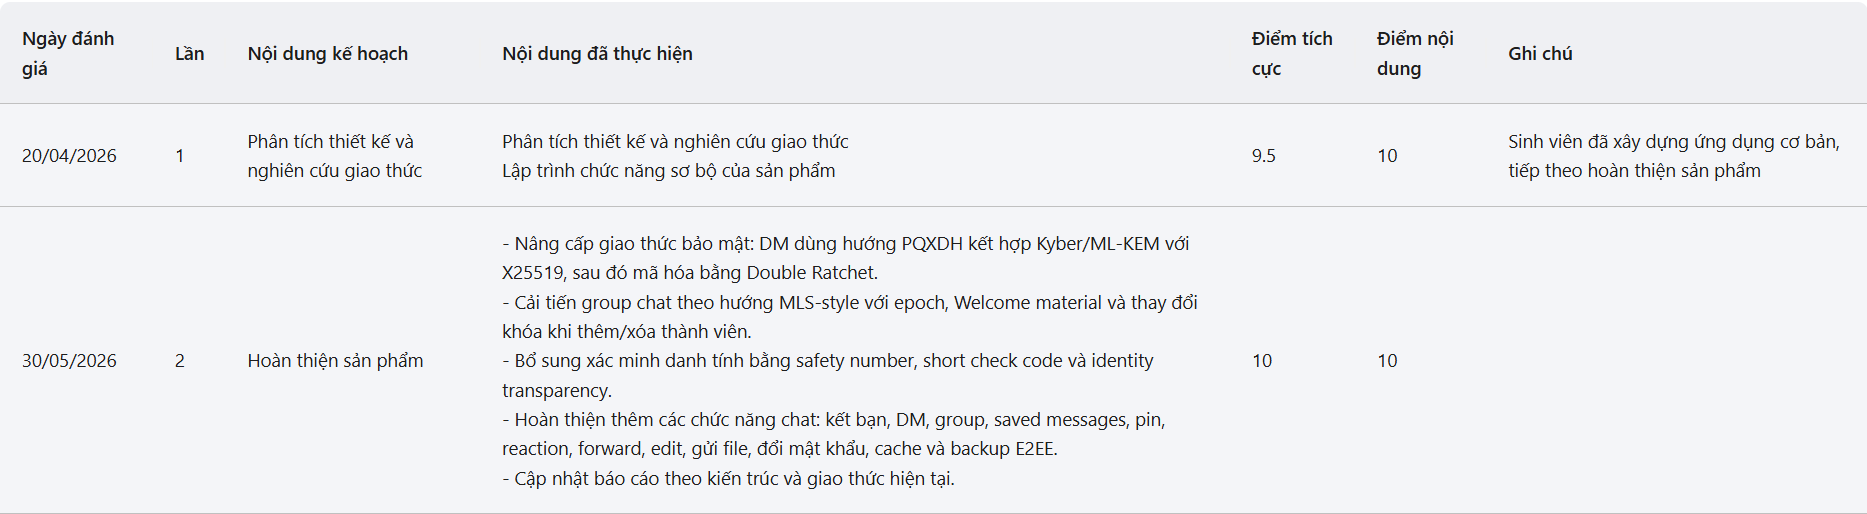
\includegraphics[width=\linewidth,height=0.85\textheight,keepaspectratio]{Figure/phieubaocao.png}%
    }{}%
    \caption*{Phiếu báo cáo tiến độ đồ án}
\end{figure}


\tableofcontents

\clearpage
\addcontentsline{toc}{chapter}{Danh sách hình vẽ}
\listoffigures

\clearpage
\addcontentsline{toc}{chapter}{Danh sách bảng}
\listoftables

\chapter*{Danh mục từ viết tắt}
\addcontentsline{toc}{chapter}{Danh mục từ viết tắt}
\markboth{Danh mục từ viết tắt}{Danh mục từ viết tắt}

\renewcommand{\arraystretch}{1.3}
\begin{longtable}{p{2.7cm} p{12.3cm}}
\textbf{Viết tắt} & \textbf{Diễn giải} \\
\hline
\endfirsthead
\multicolumn{2}{c}{\textit{(tiếp theo trang trước)}} \\
\textbf{Viết tắt} & \textbf{Diễn giải} \\
\hline
\endhead
AAD & Associated Authenticated Data -- dữ liệu được xác thực nhưng không mã hóa, đi kèm trong AEAD \\
AEAD & Authenticated Encryption with Associated Data -- mã hóa có xác thực kèm dữ liệu liên kết \\
AES & Advanced Encryption Standard -- chuẩn mã hóa khối đối xứng \\
AES-GCM & AES ở chế độ Galois/Counter Mode -- cung cấp đồng thời mã hóa và xác thực \\
AES-NI & AES New Instructions -- tập lệnh phần cứng của CPU giúp tăng tốc AES \\
ASan / UBSan & Address Sanitizer / Undefined Behavior Sanitizer -- công cụ phát hiện lỗi bộ nhớ và hành vi không xác định khi chạy mã C \\
BSD & Berkeley Software Distribution -- ở đây chỉ giao diện lập trình mạng ``socket BSD'' \\
CFFI & C Foreign Function Interface -- cơ chế cho phép Python gọi mã C \\
CRYSTALS & Cryptographic Suite for Algebraic Lattices -- bộ thuật toán mật mã trên lưới (gồm Kyber và Dilithium) \\
CVP & Closest Vector Problem -- bài toán tìm vector gần nhất trên lưới \\
DH & Diffie-Hellman -- giao thức trao đổi khóa Diffie-Hellman \\
DM & Direct Message -- tin nhắn trực tiếp giữa hai người dùng \\
E2EE & End-to-End Encryption -- mã hóa đầu cuối \\
ECDH & Elliptic Curve Diffie-Hellman -- trao đổi khóa Diffie-Hellman trên đường cong elliptic \\
ECDSA & Elliptic Curve Digital Signature Algorithm -- chữ ký số trên đường cong elliptic \\
Ed25519 & Lược đồ chữ ký số EdDSA trên đường cong Curve25519 (dùng cho khóa định danh) \\
FIPS & Federal Information Processing Standards -- bộ chuẩn xử lý thông tin liên bang Hoa Kỳ do NIST ban hành (ví dụ FIPS 203) \\
FK & Foreign Key -- khóa ngoại trong lược đồ cơ sở dữ liệu \\
FO & Fujisaki-Okamoto -- biến đổi nâng một KEM lên mức an toàn IND-CCA2 \\
FS & Forward Secrecy -- bí mật chuyển tiếp \\
HKDF & HMAC-based Key Derivation Function -- hàm dẫn xuất khóa dựa trên HMAC \\
HMAC & Hash-based Message Authentication Code -- mã xác thực thông điệp dựa trên hàm băm \\
HPKE & Hybrid Public Key Encryption -- mã hóa khóa công khai lai, dùng trong TreeKEM của MLS \\
IETF & Internet Engineering Task Force -- tổ chức tiêu chuẩn hóa Internet, ban hành các RFC \\
IKM & Input Keying Material -- vật liệu khóa đầu vào của HKDF \\
IND-CCA2 & Indistinguishability under adaptive Chosen-Ciphertext Attack -- mức an toàn chống tấn công chọn bản mã thích nghi \\
KDF & Key Derivation Function -- hàm dẫn xuất khóa \\
KEM & Key Encapsulation Mechanism -- cơ chế đóng gói khóa \\
LWE & Learning With Errors -- bài toán học kèm lỗi, nền tảng của mật mã trên lưới \\
Module-LWE & Module Learning With Errors -- biến thể LWE trên vành đa thức, nền tảng của ML-KEM \\
ML-DSA & Module-Lattice-Based Digital Signature Algorithm -- chữ ký số trên lưới (FIPS 204) \\
ML-KEM & Module-Lattice-Based Key-Encapsulation Mechanism -- KEM trên lưới (FIPS 203, tiền thân là Kyber) \\
MLS & Messaging Layer Security -- giao thức bảo mật nhắn tin nhóm (RFC 9420) \\
NIST & National Institute of Standards and Technology -- Viện Tiêu chuẩn và Công nghệ Quốc gia Hoa Kỳ \\
NP-hard & Non-deterministic Polynomial-time hard -- lớp bài toán ``khó'' trong lý thuyết độ phức tạp \\
NTT & Number Theoretic Transform -- biến đổi số học giúp tăng tốc nhân đa thức \\
OQS & Open Quantum Safe -- dự án mã nguồn mở cung cấp thư viện \texttt{liboqs} \\
PBKDF2 & Password-Based Key Derivation Function 2 -- hàm dẫn xuất khóa từ mật khẩu (RFC 8018) \\
PCS & Post-Compromise Security -- bí mật hậu thỏa hiệp \\
PK & Primary Key -- khóa chính trong lược đồ cơ sở dữ liệu \\
PQ & Post-Quantum -- (thuộc về) hậu lượng tử \\
PQC & Post-Quantum Cryptography -- mật mã hậu lượng tử \\
PQXDH & Post-Quantum Extended Diffie-Hellman -- bắt tay khóa hậu lượng tử của Signal \\
QKD & Quantum Key Distribution -- phân phối khóa lượng tử (dùng phần cứng, khác với PQC chạy bằng phần mềm) \\
RFC & Request for Comments -- tài liệu tiêu chuẩn của IETF (ví dụ RFC 9420 về MLS) \\
ROM & Random Oracle Model -- mô hình oracle ngẫu nhiên (bản lượng tử gọi là QROM) \\
RSA & Rivest-Shamir-Adleman -- hệ mật mã khóa công khai cổ điển dựa trên phân tích số nguyên \\
S3DR & Prefix tin DM của SecChat sau khi đã vào Double Ratchet \\
S3MLS & Prefix tin nhóm của SecChat, mã hóa bằng MLS \\
S3PQI & Prefix tin DM đầu phiên của SecChat, mang transcript bắt tay PQXDH \\
SHA & Secure Hash Algorithm -- họ hàm băm an toàn (ví dụ SHA-256) \\
SHAKE & Hàm băm đầu ra mở rộng thuộc họ SHA-3 (SHAKE-128, SHAKE-256) \\
SLH-DSA & Stateless Hash-Based Digital Signature Algorithm -- chữ ký số dựa trên hàm băm (FIPS 205) \\
SP & Special Publication -- ấn bản đặc biệt của NIST (ví dụ SP 800-38D, SP 800-63B) \\
SPHINCS+ & Lược đồ chữ ký số dựa trên hàm băm, nền tảng của SLH-DSA \\
SVP & Shortest Vector Problem -- bài toán tìm vector ngắn nhất trên lưới \\
TreeKEM & Cơ chế trao đổi khóa nhóm theo cây nhị phân trong MLS \\
VNC & Virtual Network Computing -- giao thức truy cập màn hình từ xa \\
X.509 & Chuẩn định dạng chứng chỉ khóa công khai (dùng trong TLS) \\
X25519 & Hàm trao đổi khóa ECDH trên đường cong Curve25519 \\
X3DH & Extended Triple Diffie-Hellman -- bắt tay khóa cổ điển của Signal (tiền thân của PQXDH) \\
X-Wing & KEM hybrid kết hợp X25519 và ML-KEM-768 (bản nháp IETF, mang tính thực nghiệm) \\
XOF & Extendable-Output Function -- hàm băm cho đầu ra độ dài tùy ý (ví dụ SHAKE) \\
\hline
\end{longtable}


\chapter*{Lời mở đầu}

Trong thập niên vừa qua, các ứng dụng nhắn tin đã trở thành phương tiện giao tiếp chủ yếu của hàng tỷ người dùng trên thế giới. Cùng với sự phát triển mạnh mẽ đó, mức độ nhạy cảm của dữ liệu được trao đổi qua các ứng dụng này cũng ngày một lớn, từ thông tin cá nhân, giao dịch tài chính cho đến các tài liệu nội bộ của tổ chức. Nhu cầu bảo mật thông tin trong quá trình truyền tải trở thành một yêu cầu bắt buộc, và mã hóa đầu cuối đã dần trở thành tiêu chuẩn trong thiết kế các nền tảng nhắn tin hiện đại như Signal, WhatsApp hay iMessage.

Tuy nhiên, phần lớn các hệ mã hóa khóa công khai đang được sử dụng hiện nay đều dựa trên các bài toán khó truyền thống như phân tích số nguyên lớn trong RSA hay bài toán logarit rời rạc trên đường cong elliptic trong ECDH. Sự xuất hiện của máy tính lượng tử cùng thuật toán Shor đã đặt ra nguy cơ rằng toàn bộ các giao thức trao đổi khóa dựa trên nền tảng này sẽ không còn an toàn trong tương lai không xa. Mối đe dọa không chỉ giới hạn ở thời điểm máy tính lượng tử thực sự xuất hiện, mà còn hiện hữu ngay lúc này qua mô hình tấn công “harvest now, decrypt later”, trong đó kẻ tấn công thu thập trước các bản mã và chờ đến khi công nghệ đủ mạnh để giải mã.

Nhằm giải quyết thách thức đó, Viện Tiêu chuẩn và Công nghệ Quốc gia Hoa Kỳ (NIST) đã tổ chức chương trình chuẩn hóa mật mã hậu lượng tử kéo dài nhiều năm, và đến năm 2024 đã công bố các chuẩn chính thức bao gồm ML-KEM, được phát triển dựa trên thuật toán Kyber. Đây là thuật toán trao đổi khóa dạng Key Encapsulation Mechanism, xây dựng trên bài toán Module Learning With Errors trong mật mã trên lưới (lattice), được thiết kế để kháng lại cả tấn công cổ điển lẫn tấn công bằng máy tính lượng tử.

Xuất phát từ bối cảnh thực tế cùng mong muốn tìm hiểu sâu hơn về mật mã học hiện đại và các công nghệ bảo mật mạng, em đã chọn đề tài “Xây dựng giao thức nhắn tin an toàn tích hợp giải pháp mật mã hậu lượng tử” để làm đồ án tốt nghiệp. Đề tài hướng tới việc khảo sát nguyên lý của các thuật toán mật mã hậu lượng tử, thiết kế một kiến trúc nhắn tin đầu cuối có bắt tay khóa hybrid hậu lượng tử, và hiện thực hóa kiến trúc này thành một ứng dụng desktop có các chức năng chính của một nền tảng nhắn tin thực tế.

Nội dung chính của đồ án bao gồm 3 chương ngoài phần mở đầu và kết luận, cụ thể:

\begin{itemize}
  \item \textbf{Chương 1: Kiến thức cơ sở}: Chương này trình bày các kiến thức nền tảng về mã hóa đầu cuối trong ứng dụng nhắn tin, mật mã đối xứng hiện đại, mối đe dọa của máy tính lượng tử đối với mật mã khóa công khai truyền thống, nguyên lý của mật mã hậu lượng tử và thuật toán ML-KEM, cùng các công nghệ được sử dụng để triển khai ứng dụng.
  \item \textbf{Chương 2: Phân tích và thiết kế hệ thống}: Chương này tập trung khảo sát các ứng dụng nhắn tin bảo mật hiện hành, phân tích yêu cầu, đề xuất kiến trúc tổng thể và trình bày thiết kế các thành phần cốt lõi của hệ thống, bao gồm cơ chế E2EE, bắt tay khóa kiểu PQXDH, Double Ratchet, group theo epoch, identity transparency, cơ sở dữ liệu, client và server.
  \item \textbf{Chương 3: Cài đặt và đánh giá hệ thống}: Chương này trình bày cách triển khai hệ thống bằng Docker, mô tả các luồng sử dụng chính, quan sát dữ liệu lưu trên server, đánh giá bảo mật, kiến trúc phần mềm, khả năng sử dụng, hiệu năng, giới hạn còn lại và các hướng phát triển tiếp theo.
\end{itemize}

Cuối cùng, em xin chân thành cảm ơn các thầy cô trong khoa Toán-Tin đã tận tình giảng dạy và trang bị cho em những kiến thức quý báu trong suốt quá trình học tập. Đặc biệt, em xin gửi lời cảm ơn sâu sắc đến thầy Trần Anh Tú đã luôn quan tâm, hướng dẫn và tạo điều kiện giúp em hoàn thành đồ án này.

\thispagestyle{fancy}


\chapter{Kiến thức cơ sở}
\section{Tổng quan về mã hóa trong ứng dụng nhắn tin}

\subsection{Mô hình đe dọa trong giao tiếp mạng}

Khi một tin nhắn được gửi đi giữa hai người dùng, dữ liệu phải đi qua nhiều thành phần trung gian trước khi đến được đích. Trên đường truyền từ thiết bị của người gửi đến máy chủ của nhà cung cấp dịch vụ, gói tin có thể bị các điểm trung gian như bộ định tuyến, nhà cung cấp dịch vụ mạng hoặc các thiết bị phân tích lưu lượng theo dõi. Ngay cả khi dữ liệu đến được máy chủ, nó vẫn có nguy cơ bị chính nhà cung cấp dịch vụ đọc, lưu trữ hoặc chuyển giao cho bên thứ ba. Đây là thực tế đã được ghi nhận trong nhiều vụ việc lộ dữ liệu người dùng từ các nền tảng nhắn tin phổ biến trong những năm gần đây.

\textbf{Tài sản cần bảo vệ.} Trong một ứng dụng nhắn tin, các tài sản chính gồm: (i) nội dung tin nhắn và tệp đính kèm; (ii) metadata như ai liên lạc với ai, vào thời điểm nào và với tần suất ra sao; (iii) danh tính và vật liệu khóa của người dùng gồm khóa định danh, các prekey và trạng thái phiên; và (iv) thông tin xác thực tài khoản như mật khẩu. Ưu tiên cao nhất là bảo vệ nội dung và vật liệu khóa, vì để lộ chúng đồng nghĩa với mất hoàn toàn tính bí mật của hội thoại.

\textbf{Các loại đối thủ.} Mô hình đe dọa chính của hệ thống nhắn tin xét các đối thủ sau:
\begin{itemize}
  \item Đối thủ nghe lén thụ động trên đường truyền (nhà cung cấp dịch vụ mạng, thiết bị trung gian, hay một chính phủ có quyền giám sát hạ tầng): đọc và lưu lại mọi gói tin nhưng không chủ động sửa đổi.
  \item Đối thủ chủ động thực hiện tấn công xen giữa: chặn, sửa, chèn hoặc phát lại gói tin, và có thể mạo danh một đầu nếu cơ chế xác thực yếu.
  \item Máy chủ vẫn tuân thủ giao thức để duy trì dịch vụ nhưng cố suy luận nội dung từ dữ liệu mà nó lưu trữ và trung chuyển. Đây chính là đối thủ trung tâm mà mã hóa đầu cuối nhắm tới, vì máy chủ có khả năng truy cập toàn bộ dữ liệu đi qua nó nếu không áp dụng mã hóa đầu cuối.
  \item Đối thủ tương lai có máy tính lượng tử thu thập bản mã hôm nay theo mô hình ``harvest now, decrypt later'' và chờ giải mã khi có đủ năng lực lượng tử.
\end{itemize}

\textbf{Giả định tin cậy.} Thiết bị đầu cuối của người dùng cùng các thư viện mật mã chạy trên đó được coi là đáng tin trong phạm vi đồ án; nếu chính thiết bị bị chiếm quyền thì khóa bí mật và bản rõ đều có thể bị lộ, điều này nằm ngoài khả năng bảo vệ của giao thức. Máy chủ không được tin để biết nội dung, nhưng vẫn được dựa vào cho tính sẵn sàng, thứ tự và việc trung chuyển tin; một máy chủ độc hại có thể chặn hoặc làm chậm tin (tấn công vào tính sẵn sàng) nhưng vẫn không đọc được nội dung đã mã hóa đầu cuối.

\subsection{Các cấp độ bảo vệ dữ liệu}

Trong thực tế, các ứng dụng nhắn tin hiện nay áp dụng nhiều cấp độ bảo vệ khác nhau với mức độ hiệu quả không đồng đều. Cấp độ cơ bản nhất là mã hóa tầng vận chuyển, thường được hiện thực hóa qua TLS. Cơ chế này chỉ bảo vệ dữ liệu trên đường truyền từ thiết bị tới máy chủ, đồng nghĩa với việc máy chủ vẫn có khả năng đọc được toàn bộ nội dung tin nhắn trước khi chuyển tiếp.

Cấp độ cao hơn là mã hóa phía máy chủ, trong đó dữ liệu được lưu trữ dưới dạng mã hóa nhưng chính máy chủ nắm giữ khóa giải mã. Phương án này bảo vệ tốt trước các rủi ro về rò rỉ dữ liệu do xâm phạm phần cứng hoặc bản sao lưu, nhưng vẫn không ngăn được việc nhân viên nội bộ hoặc cơ quan chức năng truy cập nội dung khi có yêu cầu.

Cấp độ bảo vệ cao nhất và cũng là tiêu chuẩn trong các hệ thống nhắn tin hiện đại chính là mã hóa đầu cuối. Trong mô hình này, tin nhắn được mã hóa ngay trên thiết bị của người gửi bằng khóa mà chỉ người nhận có thể giải mã. Máy chủ chỉ đóng vai trò trung chuyển các bản mã mà không có bất kỳ khả năng đọc nội dung nào. Đây là mô hình được Signal tiên phong và sau đó được WhatsApp, iMessage và nhiều nền tảng khác áp dụng.

\subsection{Yêu cầu đối với một hệ thống mã hóa đầu cuối}

Một hệ thống mã hóa đầu cuối an toàn cần đáp ứng đồng thời nhiều thuộc tính an toàn. Tính bí mật đảm bảo rằng chỉ người nhận hợp lệ mới có thể đọc được nội dung tin nhắn. Tính toàn vẹn bảo đảm rằng nội dung không bị sửa đổi trong quá trình truyền tải, đồng thời cho phép người nhận phát hiện mọi thay đổi dù nhỏ nhất. Tính xác thực cho phép người nhận xác minh chắc chắn rằng tin nhắn xuất phát từ người gửi được tuyên bố. Ngoài ra, các hệ thống tiên tiến còn hướng tới thuộc tính forward secrecy, nghĩa là ngay cả khi khóa dài hạn bị lộ trong tương lai, các phiên tin nhắn trong quá khứ vẫn không thể bị giải mã.

Để hiện thực hóa các yêu cầu trên, hệ thống cần kết hợp giữa mã hóa đối xứng cho nội dung tin nhắn với một cơ chế trao đổi khóa an toàn giữa hai đầu. Chính cơ chế trao đổi khóa là nơi mà các thuật toán mật mã khóa công khai truyền thống đang đối mặt với nguy cơ trực tiếp từ máy tính lượng tử, đòi hỏi phải được thay thế bằng những giải pháp kháng lượng tử.

\section{Mật mã đối xứng và mã hóa có xác thực}

\subsection{Thuật toán AES và chế độ GCM}

AES là một thuật toán mã hóa khối được Viện Tiêu chuẩn và Công nghệ Quốc gia Hoa Kỳ chuẩn hóa từ năm 2001 và hiện vẫn là thuật toán mã hóa đối xứng phổ biến nhất trên thế giới. AES hoạt động trên các khối dữ liệu 128-bit với độ dài khóa 128, 192 hoặc 256 bit, trong đó biến thể AES-256 cung cấp mức an toàn cao nhất. Thuật toán bao gồm nhiều vòng lặp với các thao tác thay thế, dịch hàng, trộn cột và cộng khóa vòng, tạo ra một hoán vị phụ thuộc khóa có tính kháng tấn công cao.

AES ở dạng nguyên bản chỉ định nghĩa phép mã hóa trên một khối 128-bit, do đó trong thực tế cần kết hợp với một chế độ vận hành để xử lý các thông điệp có độ dài bất kỳ. Trong các ứng dụng hiện đại, chế độ GCM là lựa chọn được khuyến nghị bởi NIST nhờ khả năng cung cấp đồng thời mã hóa và xác thực trong một thao tác duy nhất. Cấu trúc này được gọi chung là AEAD, viết tắt của Authenticated Encryption with Associated Data.

Khi vận hành AES-GCM, ngoài khóa và bản rõ, thuật toán còn cần một giá trị nonce 96-bit. Nonce phải là duy nhất đối với mỗi lần mã hóa dưới cùng một khóa, nhưng không cần bí mật và có thể được truyền công khai cùng với bản mã. Đầu ra của thuật toán bao gồm bản mã có độ dài bằng bản rõ và một thẻ xác thực 128-bit. Phía giải mã sẽ kiểm tra thẻ này trước khi trả về bản rõ, bất kỳ sự thay đổi nào trong bản mã hoặc nonce đều dẫn đến việc thẻ không hợp lệ và quá trình giải mã sẽ thất bại. Đây là một tính chất rất quan trọng giúp hệ thống tự động phát hiện tấn công sửa đổi dữ liệu mà không cần cơ chế xác thực riêng.

\subsection{Hàm dẫn xuất khóa từ mật khẩu}

Trong các ứng dụng nhắn tin sử dụng tài khoản, mật khẩu là thông tin duy nhất người dùng có thể ghi nhớ và sử dụng để thiết lập truy cập. Tuy nhiên, mật khẩu thường có entropy thấp và không thể được sử dụng trực tiếp làm khóa mã hóa, vì vậy cần một hàm dẫn xuất khóa để chuyển đổi mật khẩu thành khóa có kích thước và entropy phù hợp.

PBKDF2 là hàm dẫn xuất khóa được chuẩn hóa trong RFC 8018 và được sử dụng rộng rãi trong nhiều hệ thống bảo mật. PBKDF2 nhận đầu vào gồm mật khẩu, một giá trị salt, số vòng lặp và hàm băm cơ sở, sau đó trả về khóa dẫn xuất có độ dài mong muốn. Salt đóng vai trò quan trọng trong việc ngăn chặn tấn công sử dụng bảng băm tiền tính toán, còn số vòng lặp cao làm tăng chi phí tính toán của mỗi lần thử mật khẩu, khiến các tấn công brute-force trở nên tốn kém. Hướng dẫn lưu trữ mật khẩu của OWASP đề xuất sử dụng ít nhất 600.000 vòng khi kết hợp PBKDF2 với HMAC-SHA-256, trong khi hướng dẫn về định danh số của NIST (SP 800-63B) đưa ra các yêu cầu chung về độ mạnh và chính sách mật khẩu; cả hai cùng nhằm cân bằng giữa an toàn và trải nghiệm người dùng.

Một đặc điểm quan trọng của PBKDF2 là tính xác định. Khi đầu vào gồm mật khẩu, salt, số vòng và hàm băm không đổi, đầu ra luôn là cùng một khóa. Tính chất này cho phép ứng dụng dẫn xuất lại khóa chủ mỗi khi người dùng đăng nhập, mà không cần lưu khóa này ở bất cứ đâu.

\section{Mật mã khóa công khai truyền thống và mối đe dọa từ máy tính lượng tử}

\subsection{Nguyên lý mã hóa khóa công khai}

Khác với mã hóa đối xứng trong đó cả hai bên dùng chung một khóa bí mật, mật mã khóa công khai sử dụng một cặp khóa gồm khóa công khai và khóa bí mật. Khóa công khai có thể được phát hành rộng rãi và cho phép bất kỳ ai mã hóa thông điệp hoặc xác minh chữ ký số, trong khi khóa bí mật chỉ được người sở hữu giữ lại và dùng để giải mã hoặc ký. Cơ chế này giải quyết được bài toán trao đổi khóa trong môi trường mở, vốn là trở ngại lớn nhất của mã hóa đối xứng.

An toàn của các hệ mã hóa khóa công khai dựa trên các bài toán được cho là khó với máy tính cổ điển. Hệ RSA dựa trên độ khó của bài toán phân tích một số nguyên lớn thành tích các số nguyên tố. Các hệ mã đường cong elliptic như ECDH và ECDSA dựa trên bài toán logarit rời rạc trên nhóm điểm của đường cong elliptic, với độ khó tương đương một số bit gấp khoảng năm lần so với RSA ở cùng mức an toàn, cho phép khóa nhỏ gọn hơn đáng kể.

\subsection{Thuật toán Shor và hệ quả}

An toàn của RSA và ECDH dựa trên một giả thiết: các bài toán phân tích số nguyên và logarit rời rạc là khó đối với máy tính cổ điển. Thật vậy, cho đến nay chưa có thuật toán cổ điển nào giải được hai bài toán này trong thời gian đa thức, nên với kích thước khóa đủ lớn thì việc phá khóa bằng máy tính thông thường là bất khả thi trên thực tế. Năm 1994, Peter Shor công bố một thuật toán chạy trên máy tính lượng tử giải được cả hai bài toán đó trong thời gian đa thức, tức là phá vỡ chính giả thiết nền tảng nói trên. Hệ quả là một máy tính lượng tử đủ lớn và đủ ổn định để chạy được thuật toán Shor sẽ bẻ được khóa RSA và ECDH trong thời gian khả thi, làm sụp đổ nền tảng của toàn bộ mật mã khóa công khai đang được sử dụng hiện nay. Hệ quả này không chỉ dừng ở khâu trao đổi khóa: các lược đồ chữ ký số dựa trên cùng bài toán logarit rời rạc trên đường cong elliptic - như ECDSA hay EdDSA (Ed25519 là một biến thể phổ biến) - cũng bị Shor phá tương tự, nên cả việc xác thực bằng chữ ký số cũng không còn an toàn trước máy tính lượng tử.

Mặc dù các máy tính lượng tử hiện tại chưa đủ quy mô để thực thi Shor trên khóa có độ dài thực tế, xu hướng phát triển phần cứng lượng tử đang diễn ra rất nhanh, với các thông báo mới về số qubit và độ ổn định xuất hiện liên tục trong những năm gần đây. Chính vì vậy, cộng đồng nghiên cứu đã sớm đặt ra yêu cầu phải chuẩn bị các thuật toán thay thế trước khi máy tính lượng tử trở thành hiện thực.

Ngoài ra, có một lớp tấn công cần được tính đến ngay lập tức dù máy tính lượng tử chưa tồn tại, đó là mô hình tấn công “harvest now, decrypt later”. Trong mô hình này, kẻ tấn công thu thập và lưu trữ dữ liệu mã hóa hiện tại, chờ đến khi máy tính lượng tử đủ mạnh xuất hiện để tiến hành giải mã. Những dữ liệu có giá trị lâu dài như hồ sơ y tế, thông tin tình báo hay tài liệu pháp lý đặc biệt dễ trở thành mục tiêu. Đó là lý do các tiêu chuẩn mật mã hậu lượng tử cần được triển khai càng sớm càng tốt, ngay trong giai đoạn chuyển tiếp.

\section{Mật mã hậu lượng tử}


\subsection{Các họ thuật toán kháng lượng tử}

Mật mã hậu lượng tử là tập hợp các thuật toán được thiết kế để có thể chạy trên phần cứng cổ điển hiện có nhưng vẫn an toàn trước các tấn công từ cả máy tính cổ điển và máy tính lượng tử. Các thuật toán này được xây dựng trên các bài toán khó mà chưa có thuật toán lượng tử nào được biết đến có khả năng giải trong thời gian đa thức.

Cộng đồng nghiên cứu đã đề xuất nhiều họ thuật toán khác nhau. Họ dựa trên lưới (lattice-based) dựa trên độ khó của các bài toán trên lưới như bài toán học kèm lỗi (Learning With Errors, LWE) hay bài toán tìm vector ngắn nhất (Shortest Vector Problem, SVP), nổi bật với tính linh hoạt và hiệu năng tốt. Họ dựa trên mã (code-based) dựa trên độ khó của giải mã mã tuyến tính ngẫu nhiên, có lịch sử lâu đời từ hệ McEliece năm 1978 nhưng có nhược điểm là khóa công khai rất lớn. Họ dựa trên hàm băm (hash-based) xây dựng chữ ký số trên nền các hàm băm đã được chứng minh an toàn, ví dụ như SPHINCS+, có ưu điểm là độ tin cậy về mặt lý thuyết rất cao nhưng chữ ký lại tương đối lớn. Họ đa biến (multivariate) và họ isogeny đang được nghiên cứu nhưng còn nhiều thách thức về mặt an toàn và hiệu năng.

\subsection{Cơ sở toán học của mật mã trên lưới}

Trước khi đi vào thuật toán ML-KEM, cần nhắc lại một số khái niệm nền tảng về lưới (lattice), vốn là đối tượng toán học trung tâm cho gần như toàn bộ các đề xuất hậu lượng tử được NIST đánh giá cao nhất.

\textbf{Định nghĩa lưới (lattice).} Cho $n$ vector $\mathbf{b}_1, \mathbf{b}_2, \ldots, \mathbf{b}_n$ độc lập tuyến tính trong $\mathbb{R}^m$. Lưới $\mathcal{L}$ sinh bởi các vector này được định nghĩa là tập hợp tất cả các tổ hợp tuyến tính với hệ số nguyên:
\[
\mathcal{L}(\mathbf{b}_1, \ldots, \mathbf{b}_n) = \left\{ \sum_{i=1}^{n} x_i \mathbf{b}_i \,\middle|\, x_i \in \mathbb{Z} \right\}.
\]
Tập $\{\mathbf{b}_1, \ldots, \mathbf{b}_n\}$ được gọi là một cơ sở của lưới, còn $n$ là bậc của lưới. Về mặt hình học, lưới là một mạng các điểm phân bố đều trong không gian, và cùng một lưới có thể được biểu diễn bằng vô số cơ sở khác nhau.

\textbf{Các bài toán khó trên lưới.} Hai bài toán nền tảng được sử dụng làm cơ sở cho an toàn của mật mã trên lưới gồm:
\begin{itemize}
    \item \textbf{Bài toán tìm vector ngắn nhất (Shortest Vector Problem, SVP)}: cho một cơ sở của lưới $\mathcal{L}$, tìm vector khác không $\mathbf{v} \in \mathcal{L}$ có độ dài Euclid $\|\mathbf{v}\|$ nhỏ nhất.
    \item \textbf{Bài toán tìm vector gần nhất (Closest Vector Problem, CVP)}: cho một cơ sở của lưới $\mathcal{L}$ và một điểm $\mathbf{t} \in \mathbb{R}^m$ không thuộc lưới, tìm vector $\mathbf{v} \in \mathcal{L}$ sao cho $\|\mathbf{v} - \mathbf{t}\|$ nhỏ nhất.
\end{itemize}
Cả hai bài toán đều đã được chứng minh là NP-hard trong trường hợp chính xác và vẫn rất khó ngay cả với các phiên bản xấp xỉ. Điều đặc biệt quan trọng là cho đến nay, không có thuật toán lượng tử nào được biết giải SVP hoặc CVP trong thời gian đa thức, khác hoàn toàn với bài toán phân tích số nguyên hay logarit rời rạc mà thuật toán Shor đã giải được.

\textbf{Bài toán học kèm lỗi (Learning With Errors, LWE).} Bài toán LWE do Oded Regev đề xuất năm 2005 là cầu nối giữa các bài toán trên lưới dạng hình học nêu trên và mật mã ứng dụng. Cho $n$, $q$ là các số nguyên dương và $\chi$ là một phân phối xác suất trên $\mathbb{Z}_q$ trả về các giá trị nhỏ. Với vector bí mật $\mathbf{s} \in \mathbb{Z}_q^n$, phân phối LWE sinh các mẫu có dạng
\[
(\mathbf{a}, b) = \left(\mathbf{a}, \, \langle \mathbf{a}, \mathbf{s} \rangle + e \bmod q \right),
\]
trong đó $\mathbf{a} \in \mathbb{Z}_q^n$ được chọn đều ngẫu nhiên và $e \leftarrow \chi$ là nhiễu nhỏ. Bài toán \emph{search-LWE} yêu cầu khôi phục $\mathbf{s}$ khi biết nhiều mẫu $(\mathbf{a}_i, b_i)$, còn bài toán \emph{decision-LWE} yêu cầu phân biệt phân phối các mẫu LWE với phân phối đều. Khi viết dưới dạng ma trận với $m$ mẫu, ta có
\[
\mathbf{b} = A \cdot \mathbf{s} + \mathbf{e} \bmod q,
\]
với $A \in \mathbb{Z}_q^{m \times n}$ ngẫu nhiên và $\mathbf{e} \in \mathbb{Z}_q^m$ là vector nhiễu có các phần tử nhỏ. Nhờ công trình của Regev, bài toán decision-LWE có mức độ khó được chứng minh bằng reduction tới SVP trong trường hợp xấu nhất, nghĩa là nếu LWE giải được trong thời gian trung bình thì SVP cũng giải được trong thời gian tồi nhất. Đây là tính chất rất mạnh mà rất ít giả thiết mật mã khác có được.

\textbf{Bài toán Module-LWE.} Nếu thay không gian làm việc từ $\mathbb{Z}_q$ sang vành đa thức $R_q = \mathbb{Z}_q[X] / (X^n + 1)$ với $n$ là một lũy thừa của $2$, ta thu được biến thể Module-LWE. Các phần tử của $R_q$ là các đa thức có bậc nhỏ hơn $n$ với hệ số trong $\mathbb{Z}_q$, và phép nhân trong $R_q$ được thực hiện modulo đa thức $X^n + 1$. Bài toán Module-LWE cho một ma trận $\mathbf{A} \in R_q^{k \times k}$ và vector $\mathbf{b} = \mathbf{A} \cdot \mathbf{s} + \mathbf{e} \in R_q^k$ yêu cầu khôi phục $\mathbf{s} \in R_q^k$. Về bản chất Module-LWE là LWE đóng gói lại theo khối: thay vì một số nguyên bí mật ta có một đa thức bí mật có $n$ hệ số, và các phép nhân được thực hiện trên đa thức chứ không phải số nguyên riêng lẻ.

Ưu điểm lớn của Module-LWE là giảm đáng kể kích thước khóa so với LWE thuần, vì một phần tử của $R_q$ đã mang thông tin tương đương $n$ phần tử của $\mathbb{Z}_q$, trong khi vẫn giữ được độ khó tương đương nhờ cấu trúc đại số phong phú của vành đa thức. Đồng thời, các phép nhân đa thức có thể được tăng tốc đáng kể bằng biến đổi NTT (Number Theoretic Transform), giúp Module-LWE đạt được hiệu năng gần với các hệ mã hóa đối xứng.

\subsection{Chương trình chuẩn hóa của NIST}

Nhận thức được tầm quan trọng của việc chuẩn hóa mật mã hậu lượng tử, Viện Tiêu chuẩn và Công nghệ Quốc gia Hoa Kỳ đã khởi động chương trình tuyển chọn thuật toán từ năm 2016. Chương trình trải qua ba vòng đánh giá công khai với sự tham gia của hàng trăm nhà nghiên cứu trên toàn thế giới, mỗi thuật toán đều được xem xét về mặt toán học, hiệu năng cũng như khả năng cài đặt an toàn.

Năm 2022, NIST thông báo kết thúc vòng tuyển chọn chính và công bố các thuật toán được chọn để chuẩn hóa. Trong đó, Kyber được chọn làm thuật toán trao đổi khóa chuẩn cho mục đích mã hóa thông tin công cộng, Dilithium được chọn cho chữ ký số tổng quát, Falcon cho các trường hợp cần chữ ký ngắn, và SPHINCS+ được duy trì như một phương án dự phòng dựa trên hàm băm. Đến năm 2024, NIST chính thức công bố các tiêu chuẩn FIPS 203, 204 và 205, trong đó Kyber được chuẩn hóa dưới tên gọi ML-KEM.

Để thống nhất cách gọi trong phần còn lại của đồ án: ``Kyber'' (đầy đủ là CRYSTALS-Kyber) là tên thuật toán gốc, còn ``ML-KEM'' là tên đã được chuẩn hóa trong FIPS 203, với ba mức tham số ML-KEM-512, ML-KEM-768 và ML-KEM-1024 (tương ứng Kyber-512/768/1024). Hai tên chỉ cùng một họ thuật toán nên báo cáo dùng tên chuẩn ML-KEM và chỉ nhắc tới Kyber khi nói về thiết kế gốc. Một tên thứ ba là X-Wing, một KEM hybrid kết hợp X25519 với ML-KEM-768 được đồ án dùng cho hội thoại nhóm; khác với ML-KEM đã được chuẩn hóa, X-Wing hiện vẫn là bản nháp của IETF (\texttt{draft-connolly-cfrg-xwing-kem}) mang tính thực nghiệm, chưa phải một chuẩn đã ổn định.

\subsection{Cơ chế Key Encapsulation}

Một điểm khác biệt quan trọng của ML-KEM và nhiều thuật toán hậu lượng tử khác so với RSA là chúng thường được thiết kế dưới dạng Key Encapsulation Mechanism thay vì mã hóa bất đối xứng trực tiếp. Một KEM là bộ ba thuật toán $(\text{KeyGen}, \text{Encaps}, \text{Decaps})$ trong đó:
\begin{itemize}
    \item $\text{KeyGen}() \to (pk, sk)$: sinh cặp khóa công khai và bí mật.
    \item $\text{Encaps}(pk) \to (c, K)$: người gửi cung cấp khóa công khai của người nhận, nhận về một ciphertext $c$ và một shared secret $K$.
    \item $\text{Decaps}(sk, c) \to K$: người nhận dùng khóa bí mật của mình và ciphertext vừa nhận để khôi phục cùng shared secret $K$.
\end{itemize}
Shared secret $K$ sau đó được dùng làm khóa cho một thuật toán đối xứng như AES-GCM để mã hóa dữ liệu thực tế. Ưu điểm của cấu trúc KEM là đơn giản, có chứng minh bảo mật chặt chẽ theo mô hình IND-CCA2 và phù hợp với đặc điểm của nhiều bài toán trên lưới, nơi mà việc mã hóa trực tiếp một thông điệp tùy ý thường gặp nhiều hạn chế kỹ thuật.

\section{Thuật toán ML-KEM (Kyber)}

\subsection{Không gian làm việc và các tham số}

ML-KEM hoạt động trên vành đa thức
\[
R_q = \mathbb{Z}_q[X] / (X^n + 1),
\]
với các tham số cố định $n = 256$ và $q = 3329$. Mỗi phần tử của $R_q$ là một đa thức dạng $a_0 + a_1 X + a_2 X^2 + \cdots + a_{255} X^{255}$ trong đó các hệ số $a_i \in \mathbb{Z}_q = \{0, 1, \ldots, 3328\}$. Phép cộng trong $R_q$ đơn giản là cộng hệ số theo modulo $q$, còn phép nhân được thực hiện bằng cách nhân đa thức thông thường rồi rút gọn modulo $X^n + 1$. Do $X^n \equiv -1 \pmod{X^n+1}$, phép rút gọn này chỉ đơn thuần là hoán vị dấu các hệ số bậc cao, khiến việc cài đặt rất hiệu quả.

Tham số $q = 3329$ là một số nguyên tố đặc biệt thỏa mãn $q \equiv 1 \pmod{2n}$, cho phép vành $R_q$ tồn tại căn bậc $2n$ của đơn vị. Nhờ đó, phép nhân đa thức có thể được tăng tốc bằng biến đổi NTT, đưa độ phức tạp từ $O(n^2)$ xuống $O(n \log n)$, tương tự như vai trò của biến đổi Fourier rời rạc trong xử lý tín hiệu.

Các phiên bản ML-KEM khác nhau chỉ thay đổi tham số $k$, là số chiều của module làm việc. Cụ thể ma trận công khai $\mathbf{A}$ thuộc $R_q^{k \times k}$, còn các vector bí mật $\mathbf{s}$, nhiễu $\mathbf{e}$ và vector mã hóa thuộc $R_q^k$. Ba biến thể được sử dụng là:
\begin{itemize}
    \item ML-KEM-512 với $k = 2$, tương ứng mức an toàn NIST Level 1 (tương đương AES-128).
    \item ML-KEM-768 với $k = 3$, tương ứng mức an toàn NIST Level 3 (tương đương AES-192).
    \item ML-KEM-1024 với $k = 4$, tương ứng mức an toàn NIST Level 5 (tương đương AES-256).
\end{itemize}
Trong đồ án này, ML-KEM-768 được dùng làm ví dụ toán học vì đây là biến thể cân bằng và dễ trình bày. 

Bảng sau tóm tắt đầu vào, đầu ra và vai trò của ba thao tác chính trong ML-KEM. Đây cũng là giao diện mà ứng dụng dùng khi gọi thư viện liboqs, thay vì tự thao tác trực tiếp với đa thức bên trong thuật toán.

\begin{table}[H]
\centering
\renewcommand{\arraystretch}{1.25}
\begin{tabularx}{\linewidth}{|p{3cm}|p{3.8cm}|p{3.8cm}|X|}
\hline
\textbf{Thao tác} & \textbf{Đầu vào} & \textbf{Đầu ra} & \textbf{Vai trò trong hệ thống} \\
\hline
\texttt{KeyGen} & Nguồn ngẫu nhiên an toàn và bộ tham số thuật toán & Khóa công khai $pk$ và khóa bí mật $sk$ & Người nhận công bố $pk$ trong prekey bundle, còn $sk$ chỉ lưu cục bộ trên client. \\
\hline
\texttt{Encaps} & Khóa công khai $pk$ của người nhận & Ciphertext KEM $c$ và shared secret $K$ & Người gửi tạo một secret chung mà chỉ người giữ $sk$ tương ứng mới khôi phục được. \\
\hline
\texttt{Decaps} & Khóa bí mật $sk$ và ciphertext KEM $c$ & Shared secret $K$ hoặc một secret giả ngẫu nhiên nếu ciphertext không hợp lệ & Người nhận khôi phục secret chung để đưa vào HKDF và thiết lập khóa phiên. \\
\hline
\end{tabularx}
\caption{Đầu vào, đầu ra và vai trò của các thao tác ML-KEM}
\end{table}

\subsection{Phân phối nhiễu tâm nhị thức}

Các vector bí mật và nhiễu trong ML-KEM được lấy mẫu từ phân phối tâm nhị thức $B_\eta$, với $\eta$ là tham số nhỏ. Một mẫu $x \leftarrow B_\eta$ được sinh bằng cách lấy $2\eta$ bit ngẫu nhiên độc lập $b_1, \ldots, b_\eta, b'_1, \ldots, b'_\eta$ và tính:
\[
x = \sum_{i=1}^{\eta} (b_i - b'_i).
\]
Giá trị $x$ nằm trong khoảng $[-\eta, \eta]$ với phân phối đối xứng quanh $0$. Với ML-KEM-768, tham số $\eta_1 = 2$ được dùng cho $\mathbf{s}$ và $\mathbf{e}$ trong KeyGen, còn $\eta_2 = 2$ được dùng cho nhiễu trong Encaps. Khi mở rộng phân phối từ một số nguyên sang một đa thức thuộc $R_q$, mỗi hệ số của đa thức được lấy mẫu độc lập từ $B_\eta$, cho nên một ``đa thức nhỏ'' trong $R_q$ là một đa thức mà toàn bộ $n = 256$ hệ số đều có giá trị tuyệt đối nhỏ.

Việc chọn phân phối tâm nhị thức thay vì phân phối Gaussian rời rạc xuất phát từ nhu cầu cài đặt: $B_\eta$ chỉ cần các phép xor và đếm bit, hoàn toàn tránh được các phép tính dấu phẩy động vốn nhạy cảm với tấn công kênh kề. Về mặt bảo mật, $B_\eta$ cho độ khó Module-LWE gần như tương đương với Gaussian có phương sai tương ứng.

\subsection{Sinh khóa}

Thuật toán ML-KEM.KeyGen không nhận thông điệp của người dùng. Đầu vào thực tế của nó là nguồn ngẫu nhiên an toàn và bộ tham số như ML-KEM-768 hoặc ML-KEM-1024. Đầu ra là cặp khóa $(pk, sk)$, trong đó $pk$ được gửi lên server để người khác bắt tay, còn $sk$ phải được giữ bí mật ở client.

Các bước cốt lõi của quá trình sinh khóa như sau:

\begin{enumerate}
    \item Sinh một seed $\rho \in \{0,1\}^{256}$ và một seed $\sigma \in \{0,1\}^{256}$ độc lập, ngẫu nhiên.
    \item Mở rộng $\rho$ thành ma trận ngẫu nhiên $\mathbf{A} \in R_q^{k \times k}$ bằng hàm $\text{XOF}(\rho, i, j)$ (cụ thể là SHAKE-128), đảm bảo rằng từ cùng $\rho$ ta luôn dựng lại được cùng $\mathbf{A}$.
    \item Lấy mẫu vector bí mật $\mathbf{s} \in R_q^k$ với mỗi thành phần đa thức có các hệ số theo phân phối $B_{\eta_1}$, sử dụng seed $\sigma$ kết hợp bộ đếm.
    \item Lấy mẫu vector nhiễu $\mathbf{e} \in R_q^k$ cũng theo $B_{\eta_1}$ với seed $\sigma$ và bộ đếm tiếp theo.
    \item Tính
    \[
    \mathbf{t} = \mathbf{A} \cdot \mathbf{s} + \mathbf{e} \in R_q^k.
    \]
    \item Khóa công khai là $pk = (\mathbf{t}, \rho)$. Chỉ $\rho$ được lưu thay vì toàn bộ $\mathbf{A}$ giúp tiết kiệm không gian đáng kể.
    \item Khóa bí mật là $sk = \mathbf{s}$ (trên thực tế, phiên bản IND-CCA2 gắn thêm $pk$, hash của $pk$ và một giá trị ngẫu nhiên $z$ vào $sk$ để phục vụ biến đổi Fujisaki-Okamoto trình bày ở mục sau).
\end{enumerate}

Về mặt toán học, $(\mathbf{A}, \mathbf{t})$ chính là một thể hiện của bài toán Module-LWE: từ $\mathbf{A}$ ngẫu nhiên và $\mathbf{t} = \mathbf{A} \cdot \mathbf{s} + \mathbf{e}$, việc tìm $\mathbf{s}$ tương đương giải Module-LWE, được giả định là khó ngay cả với máy tính lượng tử.

\subsection{Encapsulate}

Thuật toán ML-KEM.Encaps là thao tác phía người gửi. Đầu vào là khóa công khai $pk = (\mathbf{t}, \rho)$ của người nhận. Đầu ra gồm ciphertext KEM $c$ để gửi qua server và shared secret $K$ dài 256 bit để đưa vào quá trình dẫn xuất khóa. 

Các bước cốt lõi gồm:

\begin{enumerate}
    \item Sinh thông điệp ngẫu nhiên $m \in \{0,1\}^{256}$.
    \item Từ $\rho$ dựng lại ma trận $\mathbf{A}$ giống hệt bên sinh khóa.
    \item Lấy mẫu ba đại lượng ngẫu nhiên phụ thuộc $m$ và $pk$:
    \begin{itemize}
        \item Vector $\mathbf{r} \in R_q^k$ với các hệ số theo $B_{\eta_1}$.
        \item Vector nhiễu $\mathbf{e}_1 \in R_q^k$ theo $B_{\eta_2}$.
        \item Nhiễu scalar $e_2 \in R_q$ theo $B_{\eta_2}$.
    \end{itemize}
    Việc lấy mẫu là xác định theo $m$ thông qua hàm băm, nên cùng một $m$ luôn sinh ra cùng $(\mathbf{r}, \mathbf{e}_1, e_2)$. Đây là chi tiết quan trọng cho biến đổi Fujisaki-Okamoto.
    \item Tính hai thành phần của ciphertext:
    \[
    \mathbf{u} = \mathbf{A}^{\top} \cdot \mathbf{r} + \mathbf{e}_1 \in R_q^k,
    \]
    \[
    v = \mathbf{t}^{\top} \cdot \mathbf{r} + e_2 + \left\lceil \tfrac{q}{2} \right\rfloor \cdot m \in R_q,
    \]
    trong đó $\lceil q/2 \rfloor$ là phần nguyên gần nhất của $q/2$ (với $q = 3329$ thì $\lceil q/2 \rfloor = 1665$), và $\lceil q/2 \rfloor \cdot m$ có nghĩa là ``gắn'' thông điệp $m$ vào hệ số của đa thức bằng cách ánh xạ bit $0$ thành hệ số $0$ và bit $1$ thành hệ số $1665$.
    \item Nén ciphertext: cả $\mathbf{u}$ và $v$ đều được nén bằng cách cắt bớt các bit thấp nhất trong mỗi hệ số, giảm kích thước truyền đi. Ký hiệu $c = (\text{Compress}(\mathbf{u}), \text{Compress}(v))$.
    \item Dẫn xuất shared secret: $K = \text{KDF}(m \,\|\, \text{Hash}(c))$, với KDF là SHAKE-256. Đây chính là khóa cuối cùng mà AES-GCM sẽ dùng.
\end{enumerate}

Trực giác toán học là như sau. Nếu bỏ qua nhiễu, ta có $\mathbf{t} = \mathbf{A} \cdot \mathbf{s}$ và $v \approx \mathbf{t}^{\top} \mathbf{r} + \lceil q/2 \rfloor m = \mathbf{s}^{\top} \mathbf{A}^{\top} \mathbf{r} + \lceil q/2 \rfloor m$. Phía giải mã biết $\mathbf{s}$, có thể tính $\mathbf{s}^{\top} \mathbf{u} \approx \mathbf{s}^{\top} \mathbf{A}^{\top} \mathbf{r}$, rồi lấy $v - \mathbf{s}^{\top} \mathbf{u}$ sẽ gần bằng $\lceil q/2 \rfloor m$. Các nhiễu nhỏ bị tích lũy trong quá trình nhưng vẫn đủ nhỏ để phục hồi được $m$ bằng cách làm tròn.

\subsection{Decapsulate}

ML-KEM.Decaps là thao tác phía người nhận. Đầu vào là khóa bí mật $sk$ đang lưu cục bộ và ciphertext KEM $c = (\mathbf{u}, v)$ nhận từ người gửi. Đầu ra là shared secret $K$ giống với phía Encaps nếu ciphertext hợp lệ. Nếu ciphertext bị sửa đổi hoặc không hợp lệ, triển khai chuẩn không trả lỗi trực tiếp mà tạo một secret giả ngẫu nhiên, giúp tránh để lộ thông tin qua phản hồi giải mã.

Các bước gồm:

\begin{enumerate}
    \item Giải nén $\mathbf{u}$ và $v$ về dạng đa thức.
    \item Tính
    \[
    w = v - \mathbf{s}^{\top} \cdot \mathbf{u} \in R_q.
    \]
    \item Khôi phục thông điệp $m'$ bằng cách làm tròn từng hệ số của $w$: hệ số gần $0$ cho bit $0$, hệ số gần $\lceil q/2 \rfloor$ cho bit $1$. Cụ thể, với mỗi hệ số $w_i \in \{0, \ldots, q-1\}$ ta đặt
    \[
    m'_i = \left\lfloor \frac{2 \cdot w_i}{q} \right\rceil \bmod 2.
    \]
    \item Chạy lại toàn bộ Encaps với $m'$ để thu được $c'$ và so sánh với ciphertext đầu vào. Nếu $c' = c$, trả về
    \[
    K = \text{KDF}(m' \,\|\, \text{Hash}(c)).
    \]
    Nếu không, trả về
    \[
    K = \text{KDF}(z \,\|\, \text{Hash}(c)),
    \]
    với $z$ là giá trị ngẫu nhiên bí mật được gắn vào $sk$ lúc sinh khóa. Kiểm tra so sánh này chính là cốt lõi của biến đổi Fujisaki-Okamoto, bảo đảm IND-CCA2.
\end{enumerate}

\subsection{Phân tích tính đúng đắn}

Để thấy vì sao quá trình giải mã khôi phục lại được $m$, xét phép tính ở bước 2 của Decaps khi bỏ qua phần nén để đơn giản:
\[
w = v - \mathbf{s}^{\top} \mathbf{u}
  = \left( \mathbf{t}^{\top} \mathbf{r} + e_2 + \lceil q/2 \rfloor m \right) - \mathbf{s}^{\top} \left( \mathbf{A}^{\top} \mathbf{r} + \mathbf{e}_1 \right).
\]
Thay $\mathbf{t}^{\top} = (\mathbf{A} \mathbf{s} + \mathbf{e})^{\top} = \mathbf{s}^{\top} \mathbf{A}^{\top} + \mathbf{e}^{\top}$ ta được:
\[
w = \mathbf{s}^{\top} \mathbf{A}^{\top} \mathbf{r} + \mathbf{e}^{\top} \mathbf{r} + e_2 + \lceil q/2 \rfloor m - \mathbf{s}^{\top} \mathbf{A}^{\top} \mathbf{r} - \mathbf{s}^{\top} \mathbf{e}_1.
\]
Rút gọn thành
\[
w = \lceil q/2 \rfloor \cdot m + \underbrace{\mathbf{e}^{\top} \mathbf{r} - \mathbf{s}^{\top} \mathbf{e}_1 + e_2}_{\text{sai số tổng hợp } \delta}.
\]
Như vậy $w$ bằng $\lceil q/2 \rfloor m$ cộng một sai số $\delta$. Do $\mathbf{e}, \mathbf{r}, \mathbf{s}, \mathbf{e}_1, e_2$ đều có hệ số nhỏ (theo phân phối $B_\eta$ với $\eta \leq 2$), kỳ vọng và phương sai của từng hệ số của $\delta$ đều được giới hạn. Các tham số $n$, $q$, $\eta_1$, $\eta_2$ và sơ đồ nén được chọn sao cho với xác suất rất cao (cụ thể, $\Pr[\text{giải mã sai}] < 2^{-164}$ với ML-KEM-768), mỗi hệ số của $\delta$ có độ lớn nhỏ hơn $q/4$. Khi đó, phép làm tròn ở bước 3 của Decaps khôi phục chính xác từng bit của $m$:
\[
m'_i = \left\lfloor \frac{2 w_i}{q} \right\rceil = \left\lfloor \frac{2 (\lceil q/2 \rfloor m_i + \delta_i)}{q} \right\rceil = m_i \bmod 2.
\]
Đây chính là lý do ML-KEM vừa đảm bảo tính đúng đắn gần như hoàn hảo, vừa giữ được mức nhiễu đủ cho Module-LWE trở thành khó.

\subsection{Biến đổi Fujisaki-Okamoto và bảo mật IND-CCA2}

ML-KEM áp dụng biến đổi Fujisaki-Okamoto để nâng lên mức bảo mật IND-CCA2 - an toàn ngay cả khi kẻ tấn công có quyền truy cập tới một oracle giải mã.

Ý tưởng của biến đổi này là thay vì mã hóa ngẫu nhiên, các giá trị $(\mathbf{r}, \mathbf{e}_1, e_2)$ được dẫn xuất xác định từ chính thông điệp $m$ và khóa công khai $pk$ thông qua hàm băm:
\[
(\mathbf{r}, \mathbf{e}_1, e_2) = G(m, pk),
\]
với $G$ là hàm băm SHAKE-256. Nhờ đó, người giải mã sau khi khôi phục $m'$ có thể tự tính lại ciphertext $c'$ một cách xác định và so sánh với $c$. Nếu $c' \neq c$, kết luận rằng ciphertext đã bị sửa đổi và trả về một khóa giả ngẫu nhiên (được dẫn xuất từ giá trị bí mật $z$) thay vì báo lỗi. Cơ chế ``giả ngẫu nhiên thay vì báo lỗi'' này được gọi là implicit rejection, giúp tránh tấn công kênh kề dạng time-based khi kẻ tấn công cố gắng phân biệt giữa ciphertext hợp lệ và không hợp lệ.

Kết quả là bộ ba $(\text{KeyGen}, \text{Encaps}, \text{Decaps})$ đầy đủ của ML-KEM đạt mức an toàn IND-CCA2 trong Random Oracle Model lượng tử, được chứng minh reduction tới độ khó Module-LWE. Đây chính là mức bảo mật mạnh nhất cần thiết cho một KEM được sử dụng thực tế, trong đó kẻ tấn công có thể vừa có khóa công khai, vừa chủ động gửi ciphertext bất kỳ để quan sát phản hồi.

\subsection{Vì sao ML-KEM phù hợp với hệ thống nhắn tin}

Đối với một ứng dụng nhắn tin, ML-KEM có ba điểm mạnh chính. Thứ nhất, thuật toán đã được NIST chuẩn hóa trong FIPS 203, nên phù hợp hơn cho một hệ thống nghiêm túc so với việc tự chọn một đề xuất chưa ổn định. Thứ hai, đầu ra của ML-KEM là một shared secret ngắn, dễ đưa vào HKDF để kết hợp với X25519, Double Ratchet hoặc cơ chế MLS group. Thứ ba, thao tác encapsulate và decapsulate đủ nhanh để chạy trên client desktop mà không tạo độ trễ rõ rệt cho người dùng.

ML-KEM không dùng để mã hóa trực tiếp nội dung tin nhắn. Ciphertext KEM chỉ có nhiệm vụ vận chuyển một secret dùng cho bắt tay. Sau khi secret được tạo, nội dung tin nhắn vẫn nên được mã hóa bằng thuật toán đối xứng như AES-GCM. Cách tách vai trò này giúp hệ thống đơn giản hơn: KEM giải quyết bài toán thiết lập secret ban đầu, còn AEAD giải quyết bài toán mã hóa và xác thực từng message.

\subsection{Các biến thể và mức an toàn}

ML-KEM được cung cấp ở ba biến thể tương ứng với ba mức an toàn khác nhau. ML-KEM-512 với $k=2$ cung cấp mức an toàn tương đương AES-128, phù hợp cho các ứng dụng hạn chế về tài nguyên. ML-KEM-768 với $k=3$ cung cấp mức an toàn tương đương AES-192, là lựa chọn cân bằng giữa an toàn và hiệu năng, và được khuyến nghị cho đa số ứng dụng thực tế. ML-KEM-1024 với $k=4$ đạt mức an toàn tương đương AES-256 và phù hợp cho các ứng dụng có yêu cầu bảo mật cao nhất.

Về kích thước, ML-KEM-768 có khóa công khai 1184 byte, khóa bí mật 2400 byte, ciphertext 1088 byte và shared secret 32 byte. Các giá trị này lớn hơn đáng kể so với ECDH trên đường cong X25519 với khóa chỉ 32 byte, nhưng vẫn trong giới hạn có thể chấp nhận đối với một ứng dụng desktop hiện đại. Bù lại, thời gian thực thi của ML-KEM ở các thao tác keygen, encapsulate và decapsulate đều rất nhanh, thường chỉ trong khoảng vài trăm micro giây trên một CPU phổ thông.

\section{Forward secrecy, Double Ratchet và MLS}

\subsection{Forward secrecy và post-compromise security}

Forward secrecy là thuộc tính bảo đảm rằng việc lộ một khóa dài hạn ở thời điểm sau không tự động làm lộ các tin nhắn đã gửi trước đó. Trong nhắn tin, yêu cầu này quan trọng vì transcript có thể bị lưu lại rất lâu bởi mạng, server hoặc bản sao lưu. Nếu hệ thống dùng một khóa hội thoại cố định cho toàn bộ lịch sử, chỉ cần khóa đó bị lộ thì toàn bộ transcript cũ đều nguy hiểm.

Post-compromise security là thuộc tính mạnh hơn ở chiều ngược lại. Nếu attacker từng lấy được một phần trạng thái tạm thời trên thiết bị nhưng sau đó không còn kiểm soát thiết bị nữa, giao thức cần có khả năng tự phục hồi sau khi hai bên tiếp tục trao đổi secret mới. Hai thuộc tính này không đến từ một thuật toán đơn lẻ, mà đến từ cách tổ chức vòng đời khóa: khóa message chỉ dùng một lần, chain key được cập nhật liên tục, và các secret mới được đưa vào state theo thời gian.

\subsection{Double Ratchet trong hội thoại hai người}\label{subsec:theory-dr}

Double Ratchet là cơ chế đạt forward secrecy ở mức từng tin nhắn cho hội thoại hai người, được phổ biến qua giao thức Signal. Sau bước bắt tay ban đầu, hai phía cùng có một \emph{root key} bí mật chung. Toàn bộ phần còn lại của giao thức xoay quanh việc liên tục biến đổi root key này thành các khóa con dùng một lần, theo hai ``bánh cóc'' (ratchet) lồng nhau: một bánh cóc đối xứng chạy theo từng tin, và một bánh cóc Diffie-Hellman chạy theo từng lượt đổi chiều. Sở dĩ gọi là bánh cóc vì giống cơ cấu cơ khí chỉ quay được một chiều: trạng thái khóa chỉ tiến tới, không thể quay ngược lại để khôi phục các giá trị cũ.

\textbf{Trạng thái phiên.} Ở mỗi phía, mỗi cuộc hội thoại được mô tả bằng một trạng thái phiên  ($\mathsf{st}$) - là toàn bộ vật liệu khóa và bộ đếm cần để mã hóa tin kế tiếp và giải mã tin nhận về:
\[
  \mathsf{st} = \bigl(RK,\ CK_s,\ CK_r,\ (pk_{\text{self}}, sk_{\text{self}}),\ pk_{\text{remote}},\ N_s,\ N_r,\ PN,\ \mathsf{MK}_{\text{skip}}\bigr).
\]
Ý nghĩa và vai trò của từng thành phần:
\begin{itemize}
  \item $RK$ - \emph{root key}, bí mật gốc của phiên (ban đầu do bắt tay PQXDH gieo). Nó chỉ thay đổi khi có bánh cóc DH nên đóng vai trò trục ổn định giữa các lượt đổi chiều, và là nguồn dẫn ra mọi chain key.
  \item $CK_s,\ CK_r$ - hai \emph{chain key} cho chiều gửi và chiều nhận, mỗi tin tiến một bước qua $\mathrm{KDF\_CK}$. Vì hai phía cùng một $RK$ nhưng tráo vai nên chain gửi của bên này đúng bằng chain nhận của bên kia.
  \item $(pk_{\text{self}}, sk_{\text{self}})$ - cặp khóa X25519 ratchet hiện hành của mình; khóa công khai $pk_{\text{self}}$ được đính vào header mỗi tin gửi đi.
  \item $pk_{\text{remote}}$ - khóa ratchet công khai mới nhất của đối phương. Khi header một tin đến mang khóa khác giá trị này, đó là tín hiệu để thực hiện một bước DH ratchet.
  \item $N_s,\ N_r$ - số tin đã gửi trong chain gửi hiện tại, và số thứ tự tin mong đợi tiếp theo ở chain nhận.
  \item $PN$ - (\emph{previous N}) độ dài chain gửi trước lần xoay DH ratchet gần nhất. Nhờ $PN$ đặt trong header, phía nhận biết phải sinh và lưu nốt bao nhiêu khóa của chain cũ trước khi chuyển sang chain mới, để các tin cũ đến muộn vẫn giải mã được.
  \item $\mathsf{MK}_{\text{skip}}$ - bảng message key của các tin bị bỏ qua (đến muộn hoặc lệch thứ tự), có giới hạn kích thước để chống bị làm cạn bộ nhớ.
\end{itemize}
Mọi khóa trong $\mathsf{st}$ đều dài 32 byte (root key, chain key, message key và khóa X25519). Cài đặt thực tế còn bổ sung vài trường để ràng buộc metadata (khóa mã hóa header, định danh phiên và hội thoại, số thứ tự định danh) cùng cơ chế chống nhận lặp, nhưng không làm thay đổi bản chất hai bánh cóc.

\textbf{Bánh cóc đối xứng (symmetric-key ratchet).} Từ root key, mỗi phía dẫn xuất hai \emph{chain key}: một cho chiều gửi và một cho chiều nhận. Mỗi khi cần xử lý một tin, chain key được đưa qua một hàm dẫn xuất một chiều $\mathrm{KDF\_CK}$ để tách ra đồng thời một \emph{message key} dùng một lần và một chain key kế tiếp:
\[
  MK_i = \mathrm{HMAC}(CK_i, \texttt{0x01}), \qquad
  CK_{i+1} = \mathrm{HMAC}(CK_i, \texttt{0x02}).
\]
Message key $MK_i$ chỉ dùng để mã hóa hoặc giải mã đúng một tin rồi bị xóa; chain key tiến từ $CK_i$ sang $CK_{i+1}$ và giá trị cũ cũng bị xóa ngay. Vì $\mathrm{HMAC}$ là một chiều, biết $CK_{i+1}$ hay $MK_i$ không cho phép suy ngược ra $CK_i$ hoặc bất kỳ message key nào trước đó. Đây chính là nguồn gốc của forward secrecy ở mức tin nhắn: việc lộ trạng thái hiện tại không làm lộ các tin đã gửi trước.

\textbf{Bánh cóc Diffie-Hellman (DH ratchet).} Riêng bánh cóc đối xứng thì không tự phục hồi: nếu attacker lấy được chain key hiện tại, hắn có thể tính mọi message key về sau trong cùng một chiều. Để vá điểm này, mỗi phía giữ thêm một cặp khóa DH tạm thời và đính kèm khóa công khai DH hiện hành của mình vào header mỗi tin. Khi một phía nhận được một khóa DH công khai mới của đối phương, nó thực hiện một bước DH ratchet: tính một secret DH mới rồi trộn vào root key để sinh ra root key và chain key mới qua hàm $\mathrm{KDF\_RK}$:
\[
  RK' \,\Vert\, CK' = \mathrm{HKDF}\bigl(\,\text{salt}=RK,\ \ \text{IKM}=\mathrm{DH}(sk_{\text{self}}, pk_{\text{remote}}),\ \ \texttt{info},\ 64\,\bigr).
\]
Đầu ra 64 byte được cắt làm đôi: 32 byte đầu là root key mới $RK'$, 32 byte sau là chain key mới $CK'$ cho chiều vừa thiết lập; \texttt{info} là một nhãn cố định gắn với ứng dụng. Bên trong, $\mathrm{HKDF}$ gồm bước Extract (dùng $RK$ làm salt để trộn DH secret thành một khóa giả ngẫu nhiên) rồi bước Expand (kéo dài thành 64 byte có cấu trúc). Sau đó phía này tự sinh một cặp khóa DH mới cho riêng mình và gửi kèm khóa công khai trong tin tiếp theo, để đối phương cũng thực hiện bước ratchet tương ứng. Nhờ liên tục bơm secret DH tươi vào root key, giao thức đạt post-compromise security: chỉ cần hai bên còn trao đổi được một lượt khóa DH mới mà attacker không quan sát, trạng thái sẽ ``lành lại'' và các tin sau đó an toàn trở lại.

\textbf{Thuật toán gửi và nhận một tin.} Khi gửi, phía gửi tiến chain key gửi để lấy message key, gắn header rồi mã hóa bằng AEAD với header làm dữ liệu xác thực kèm theo (AAD):
\begin{enumerate}
  \item $(CK_s,\ MK) \leftarrow \mathrm{KDF\_CK}(CK_s)$ và tăng $N_s$;
  \item dựng header $H = (pk_{\text{self}},\ PN,\ N_s)$;
  \item $c = \mathrm{AEAD.Enc}\bigl(MK;\ \text{plaintext};\ \mathsf{AAD}=H\bigr)$, rồi xóa ngay $MK$.
\end{enumerate}
Khi nhận một tin có header $H' = (pk',\ PN',\ N')$: nếu $pk'$ khác $pk_{\text{remote}}$ đang lưu thì trước hết sinh và cất các message key còn thiếu của chain cũ tới chỉ số $PN'$, rồi thực hiện một \emph{bước DH ratchet} (tính $RK,\ CK_r$ mới theo công thức trên, sinh cặp khóa DH mới và đặt lại $N_s=N_r=0$). Tiếp đó phía nhận tiến chain nhận tới chỉ số $N'$, lưu các message key trung gian vào $\mathsf{MK}_{\text{skip}}$, lấy ra $MK$ rồi giải mã và kiểm tra tag AEAD trên cả header lẫn ciphertext. Việc đưa header vào AAD ràng buộc mỗi ciphertext với đúng khóa DH và chỉ số của nó, nên kẻ tấn công không thể tráo header để đánh lừa bước ratchet.

\textbf{Tin lệch thứ tự và chống lặp.} Vì mạng có thể giao tin sai thứ tự, header còn mang hai bộ đếm: số thứ tự của tin trong chain hiện tại và số tin của chain trước đó. Khi nhận một tin có số thứ tự vượt trước, phía nhận lần lượt sinh và lưu tạm các message key bị bỏ qua (\emph{skipped keys}) trong một giới hạn an toàn để vẫn giải mã được tin đến muộn, đồng thời từ chối ciphertext đã dùng nhằm chống replay. Trong đồ án, giới hạn này là 1000 khóa để cân bằng giữa khả năng chịu lệch thứ tự và rủi ro bị làm cạn bộ nhớ.

\textbf{Liên hệ hậu lượng tử.} Bản thân bánh cóc dùng X25519 nên không kháng lượng tử; tính kháng lượng tử của hội thoại nằm ở bước bắt tay ban đầu, nơi root key đầu tiên được gieo từ một bắt tay kiểu PQXDH có trộn thêm shared secret ML-KEM (trình bày ở chương thiết kế). Nói cách khác, ML-KEM bảo vệ bí mật của điểm khởi đầu, còn Double Ratchet bảo vệ tiến trình của hội thoại theo thời gian.

\subsection{Messaging Layer Security cho hội thoại nhóm}\label{subsec:theory-mls}

Nếu áp dụng Double Ratchet riêng cho từng cặp thành viên trong một nhóm $n$ người, mỗi tin phải mã hóa lại $n-1$ lần và số phiên cần đồng bộ tăng theo $O(n^2)$; việc thêm/xóa thành viên và giữ đúng các thuộc tính an toàn trở nên rất khó. Messaging Layer Security (MLS, RFC 9420) giải bài toán này bằng một \emph{group state} chung, cho phép làm mới khóa nhóm với chi phí chỉ $O(\log n)$ cho mỗi thao tác.

\textbf{Cây ratchet và TreeKEM.} Trái tim của MLS là một cây nhị phân cân bằng gọi là \emph{ratchet tree}: mỗi thành viên là một lá, mỗi nút (kể cả nút trong) gắn với một cặp khóa bất đối xứng. Bất biến cốt lõi của TreeKEM là: một thành viên biết khóa bí mật của đúng những nút nằm trên đường đi trực tiếp từ lá của mình lên gốc (\emph{direct path}), và biết khóa công khai của mọi nút còn lại. Khóa bí mật của nút gốc do đó là một secret mà toàn bộ và chỉ các thành viên hiện tại mới cùng suy ra được.

Cây được đánh số theo thứ tự duyệt giữa (in-order): với $n$ lá, cây có $2n-1$ nút, lá ở các chỉ số chẵn còn nút trong ở các chỉ số lẻ; cha và hai con của một nút được xác định thuần túy bằng số học trên chỉ số, nên mọi thành viên cùng nhìn thấy một cấu trúc cây thống nhất mà không phải trao đổi thêm. Direct path của một lá là dãy nút từ cha trực tiếp lên gốc; \emph{copath} là dãy các nút anh em của những nút đó (phần cây con ở phía đối diện).

\textbf{Cập nhật đường đi (path update).} Khi một thành viên làm mới khóa của mình (thao tác Update) hoặc khi có thay đổi thành viên, nó sinh một secret lá ngẫu nhiên $s_0$ rồi dẫn ra một chuỗi \emph{path secret} dọc theo direct path; tại mỗi mức, path secret vừa sinh ra cặp khóa HPKE của nút đó, vừa dẫn tiếp lên mức cha:
\[
  s_{i} = \mathrm{DeriveSecret}(s_{i-1},\ \mathtt{path}), \qquad
  (pk_i, sk_i) = \mathrm{DeriveKeyPair}\bigl(\mathrm{DeriveSecret}(s_i,\ \mathtt{node})\bigr),
\]
trong đó $\mathrm{DeriveSecret}(s, L) = \mathrm{ExpandWithLabel}(s, L, \varepsilon, N_h)$ là HKDF-Expand có gắn nhãn $L$ (độ dài đầu ra $N_h$ byte). Để các thành viên khác cập nhật theo, với mỗi nút $v$ trên direct path, người cập nhật mã hóa path secret tương ứng cho \emph{tập độ phân giải} (resolution) của copath bằng HPKE:
\[
  \mathsf{ct}_v = \mathrm{HPKE.Enc}\bigl(pk_{\mathrm{res}(v)},\ s_{i(v)}\bigr).
\]

Một thành viên khác giải mã được $\mathsf{ct}_v$ tại đúng điểm hai đường đi gặp nhau (nút tổ tiên chung thấp nhất), rồi tự dẫn tiếp các path secret còn lại lên gốc bằng chính công thức trên. Nhờ chỉ phải mã hóa cho $O(\log n)$ nút thay vì cho từng người, chi phí một lần cập nhật giảm từ tuyến tính xuống còn logarit theo số thành viên.

\textbf{Lịch khóa và epoch.} Mỗi cấu hình nhóm là một \emph{epoch}. Sau một thao tác, secret rút ra từ gốc cây (\emph{commit secret}) được trộn với init secret của epoch trước qua hai bước HKDF để tạo joiner secret rồi epoch secret:
\[
  \text{joiner}_n = \mathrm{KDF.Extract}\bigl(\text{init}_{n-1},\ \text{commit}_n\bigr),
\]
\[
  \text{epoch}_n = \mathrm{ExpandWithLabel}\bigl(\mathrm{KDF.Extract}(\text{joiner}_n,\ \text{psk}),\ \mathtt{epoch},\ \mathrm{GroupContext}_n,\ N_h\bigr),
\]
trong đó $\text{psk}$ là pre-shared key (bằng 0 nếu không dùng) và $\mathrm{GroupContext}_n$ buộc khóa vào đúng cấu hình nhóm ở epoch $n$. Từ $\text{epoch}_n$, mỗi secret chuyên biệt được dẫn ra bằng $\mathrm{DeriveSecret}(\text{epoch}_n, L)$ với một nhãn $L$ riêng, trong đó đáng chú ý là:
\begin{itemize}
  \item \texttt{encryption} - gốc của \emph{secret tree} sinh khóa mã hóa tin ứng dụng;
  \item \texttt{sender data} - bảo vệ metadata định danh người gửi của mỗi tin;
  \item \texttt{confirm} và \texttt{membership} - khóa xác thực transcript và tư cách thành viên trong handshake;
  \item \texttt{init} - chính là $\text{init}_n$, được nối làm đầu vào cho key schedule của epoch kế tiếp.
\end{itemize}
Việc init secret của epoch này nối tiếp vào epoch sau tạo thành một bánh cóc bất đối xứng ở quy mô nhóm: mỗi lần đổi epoch, toàn bộ khóa cũ bị bỏ (forward secrecy) và entropy mới từ commit secret được bơm vào (post-compromise security).

\textbf{Cây secret và bánh cóc ứng dụng trong một epoch.} Riêng việc đổi epoch chỉ cho forward secrecy ở mức thô. Để mỗi tin trong cùng một epoch cũng có khóa riêng, secret nhãn \texttt{encryption} được dùng làm gốc của một cây nhị phân thứ hai gọi là \emph{secret tree}; mỗi lá ứng với một thành viên và cho ra một chuỗi ratchet đối xứng riêng. Tại thế hệ $j$, khóa và nonce AEAD cùng secret kế tiếp được dẫn ra bằng HKDF có nhãn:

\begin{itemize}
  \item Khóa AEAD: $k_j = \mathrm{ExpandWithLabel}(r_j, \mathtt{key}, j, N_k)$;
  \item Nonce AEAD: $n_j = \mathrm{ExpandWithLabel}(r_j, \mathtt{nonce}, j, N_n)$;
  \item Secret kế tiếp: $r_{j+1} = \mathrm{ExpandWithLabel}(r_j, \mathtt{secret}, j, N_h)$.
\end{itemize}

Mỗi tin dùng một cặp $(k_j, n_j)$ riêng rồi $r_j$ tiến tới $r_{j+1}$ và bị xóa, cho forward secrecy theo từng tin ngay trong một epoch. Như vậy MLS đạt cả hai thuộc tính theo hai trục bổ sung nhau: bánh cóc đối xứng trong secret tree lo forward secrecy giữa các tin, còn bánh cóc bất đối xứng qua các epoch (path update) lo post-compromise security ở mức nhóm.

\textbf{Đề xuất, Commit và Welcome.} Thay đổi nhóm được biểu diễn bằng các \emph{proposal}: Add (thêm thành viên qua KeyPackage của họ), Remove (xóa thành viên), Update (làm mới khóa của một thành viên). Một \emph{Commit} gói một tập proposal lại, thực hiện path update và đẩy nhóm sang epoch mới. Thành viên mới nhận một thông điệp \emph{Welcome} chứa đủ secret (mã hóa riêng cho KeyPackage của họ) để bước vào đúng epoch; thành viên bị Remove không nằm trong tập nhận secret của epoch kế tiếp nên lập tức mất khả năng giải mã.

\textbf{Tách public state và secret state.} MLS phân biệt rõ phần công khai và phần bí mật của group state. Các phần public như GroupInfo, cấu trúc ratchet tree (chỉ gồm khóa công khai), epoch và danh sách credential cho phép kiểm tra tính nối tiếp và hợp lệ của nhóm mà không lộ application secret; các secret như epoch secret và path secret chỉ tồn tại ở client. Nhờ vậy một server không tin cậy vẫn có thể lưu trữ, chuyển tiếp và kiểm tra ràng buộc membership dựa trên public state, nhưng không bao giờ giải mã được tin nhắn nhóm.

\section{Giao thức TLS và vai trò trong kiến trúc bảo mật}

Mặc dù mã hóa đầu cuối đã bảo vệ nội dung tin nhắn khỏi server, TLS ở tầng vận chuyển vẫn có ý nghĩa quan trọng trong một kiến trúc bảo mật nhiều lớp. TLS che nội dung gói JSON khỏi người nghe lén trên mạng và giúp xác thực máy chủ ở cấp độ hạ tầng. Tuy nhiên TLS không che hoàn toàn metadata như địa chỉ kết nối, thời điểm truyền và kích thước gói quan sát được trên mạng. Khi kết hợp mã hóa đầu cuối với TLS, hệ thống có hai lớp phòng vệ khác nhau thay vì chỉ phụ thuộc vào một lớp.

Trong đồ án, tầng TLS giữa client và server được thiết lập với chứng chỉ X.509. Toàn bộ các gói JSON được gửi trong kênh TLS này, bao gồm cả những gói đã chứa ciphertext đầu cuối. Nhờ đó, kẻ tấn công trên đường truyền không đọc được nội dung JSON. Dù vậy, server vẫn là điểm cuối của TLS, nên nội dung chat vẫn phải được mã hóa thêm ở tầng ứng dụng bằng E2EE.

\section{Các công nghệ triển khai}

\subsection{Ngôn ngữ Python và PyQt5}

Python là ngôn ngữ được lựa chọn để hiện thực hóa phía client nhờ vào sự kết hợp giữa cú pháp rõ ràng, hệ sinh thái thư viện phong phú và khả năng tích hợp tốt với các thành phần mật mã. Đối với phần giao diện, PyQt5 là framework trưởng thành và ổn định, cung cấp binding đầy đủ của thư viện Qt cho Python, cho phép xây dựng giao diện desktop native trên cả Windows, Linux và macOS từ cùng một mã nguồn.

PyQt5 hỗ trợ kiến trúc signal-slot, rất phù hợp cho các ứng dụng mạng bất đồng bộ, nơi các sự kiện từ luồng mạng cần được truyền về luồng giao diện một cách an toàn. Framework cũng cung cấp nhiều thành phần trực quan sẵn có như QScrollArea, QWidget, QListWidget, QFileDialog và nhiều widget khác để xây dựng message list, danh sách liên lạc, chọn file và các dialog chức năng.

\subsection{Ngôn ngữ C và thư viện hệ thống}

Phía máy chủ được triển khai bằng ngôn ngữ C để đảm bảo hiệu năng cao, mức sử dụng tài nguyên thấp và khả năng kiểm soát bộ nhớ chi tiết. Một máy chủ nhắn tin phải xử lý đồng thời nhiều kết nối mạng, mỗi kết nối có thể truyền tải các gói tin kích thước rất khác nhau từ tin nhắn văn bản ngắn vài byte cho đến file đa phương tiện nhiều megabyte. C cho phép quản lý bộ nhớ động một cách chính xác, tránh được chi phí của garbage collector và tận dụng tối đa các hệ thống lập lịch luồng của hệ điều hành.

Server trong đồ án sử dụng các thư viện hệ thống chuẩn của Linux bao gồm pthread cho mô hình đa luồng, socket BSD cho lập trình mạng, và OpenSSL cho tầng TLS. Ngoài ra, MySQL Connector/C được sử dụng để kết nối tới cơ sở dữ liệu, và một parser JSON nhẹ được viết thủ công để phân tích các gói tin mà không phụ thuộc vào thư viện bên ngoài nặng nề.

\subsection{Thư viện Open Quantum Safe}

Để tích hợp ML-KEM vào ứng dụng, đồ án sử dụng thư viện Open Quantum Safe, một dự án mã nguồn mở cung cấp hiện thực hóa các thuật toán mật mã hậu lượng tử đang được chuẩn hóa hoặc trong quá trình đánh giá. Thư viện lõi liboqs được viết bằng C với các tối ưu hóa cho nhiều kiến trúc CPU khác nhau, đồng thời cung cấp binding cho các ngôn ngữ phổ biến bao gồm Python, C++, Java và Go.

Trong đồ án, binding Python oqs-python được sử dụng ở phía client để thực hiện các thao tác KEM cần thiết như sinh khóa, encapsulate và decapsulate. Việc sử dụng một thư viện đã được kiểm định và duy trì tích cực là điều quan trọng, bởi mật mã hậu lượng tử có nhiều chi tiết cài đặt tinh tế mà việc tự viết lại từ đầu có thể dẫn đến các lỗi bảo mật khó phát hiện.

\subsection{Thư viện cryptography và các thao tác AES-GCM}

Đối với mã hóa đối xứng AES-GCM và hàm dẫn xuất khóa PBKDF2, thư viện cryptography của Python được lựa chọn. Đây là thư viện mật mã chính thức được cộng đồng Python Cryptographic Authority phát triển, cung cấp cả giao diện cấp cao dễ sử dụng và giao diện cấp thấp cho người cần kiểm soát chi tiết. Thư viện được xây dựng trên nền OpenSSL với các ràng buộc CFFI, đảm bảo hiệu năng gần bằng cài đặt C thuần và tự động hưởng lợi từ các tăng tốc phần cứng như AES-NI trên các CPU hỗ trợ.

\subsection{Cơ sở dữ liệu MySQL}

MySQL được chọn làm cơ sở dữ liệu quan hệ do tính phổ biến, tài liệu phong phú và hiệu năng tốt trong các tác vụ ghi-đọc nhiều. Ứng dụng nhắn tin có mô hình dữ liệu tương đối đơn giản với các thực thể như người dùng, bạn bè, hội thoại và tin nhắn, rất phù hợp với mô hình quan hệ. MySQL cũng hỗ trợ kiểu dữ liệu LONGTEXT lên tới 4 GB cho mỗi bản ghi, rất có ích khi lưu trữ tin nhắn chứa file đã được mã hóa và mã hóa base64 với độ dài có thể lên tới vài chục megabyte.

\subsection{Docker và Docker Compose}

Để đơn giản hóa việc triển khai và đảm bảo môi trường chạy nhất quán giữa các máy phát triển khác nhau, đồ án sử dụng Docker làm công cụ container hóa cùng Docker Compose để điều phối nhiều container. Server C và MySQL được đóng gói thành hai container riêng biệt với các volume lưu trữ bền vững cho dữ liệu cơ sở dữ liệu. Với một lệnh docker compose up duy nhất, toàn bộ môi trường máy chủ có thể được khởi động, tạo điều kiện thuận lợi cho việc phát triển, kiểm tra nội bộ và trình diễn.


\newpage
\chapter{Phân tích và thiết kế hệ thống}

\section{Khảo sát thực tế}

\subsection{Thực trạng các giao thức nhắn tin mã hóa đầu cuối}

Sự phổ biến của các ứng dụng nhắn tin trực tuyến đã kéo theo nhu cầu ngày càng cao về bảo vệ quyền riêng tư và tính bảo mật của dữ liệu trao đổi. Để đáp ứng yêu cầu đó, mã hóa đầu cuối (End-to-End Encryption - E2EE) đã trở thành cơ chế bảo mật cốt lõi trong nhiều nền tảng nhắn tin hiện đại. Với E2EE, nội dung tin nhắn được mã hóa tại thiết bị người gửi và chỉ được giải mã tại thiết bị người nhận, giúp ngăn chặn việc đọc trộm dữ liệu bởi máy chủ trung gian hoặc các bên thứ ba.

Hiện nay, nhiều ứng dụng nhắn tin phổ biến đã triển khai E2EE dưới các hình thức khác nhau. Trong đó, Signal được xem là một trong những nền tảng tiên phong với Signal Protocol, giao thức đã trở thành cơ sở cho cơ chế bảo mật của WhatsApp, Google Messages và nhiều hệ thống liên lạc khác. Các giao thức này không chỉ cung cấp tính bí mật của nội dung trao đổi mà còn hỗ trợ các thuộc tính an toàn quan trọng như xác thực người dùng, bí mật chuyển tiếp (Forward Secrecy) và bí mật hậu thỏa hiệp (Post-Compromise Security).

Bên cạnh việc bảo vệ nội dung tin nhắn, các giao thức hiện đại còn phải giải quyết nhiều yêu cầu phức tạp hơn như đồng bộ trên nhiều thiết bị, hỗ trợ người dùng ngoại tuyến, quản lý khóa phiên động và đảm bảo hiệu năng khi số lượng người dùng tăng cao. Điều này khiến thiết kế giao thức nhắn tin trở thành một bài toán tổng hợp giữa mật mã học, kiến trúc hệ thống và trải nghiệm người dùng.

\subsection{Các cơ chế bảo mật được sử dụng trong hệ thống nhắn tin hiện nay}

Phần lớn các hệ thống E2EE hiện nay áp dụng mô hình mật mã lai (Hybrid Cryptography), trong đó mật mã khóa công khai được sử dụng để thiết lập khóa phiên và mật mã đối xứng được sử dụng để mã hóa dữ liệu thực tế.

Trong Signal Protocol, quá trình thiết lập khóa ban đầu được thực hiện thông qua Extended Triple Diffie-Hellman (X3DH), cho phép hai người dùng tạo khóa chung ngay cả khi một bên đang ngoại tuyến. Sau khi khóa ban đầu được thiết lập, cơ chế Double Ratchet được sử dụng để liên tục cập nhật khóa phiên sau mỗi lần trao đổi tin nhắn. Nhờ đó, việc lộ khóa ở một thời điểm không làm ảnh hưởng đến toàn bộ lịch sử liên lạc.

Mô hình này đã chứng minh được hiệu quả trong thực tế và hiện được xem là tiêu chuẩn tham chiếu cho việc xây dựng các ứng dụng nhắn tin bảo mật. Tuy nhiên, nền tảng trao đổi khóa của các giao thức này vẫn chủ yếu dựa trên mật mã đường cong elliptic, vốn được thiết kế cho môi trường tính toán cổ điển.

\subsection{Những thách thức trong thiết kế giao thức nhắn tin thế hệ mới}

Mặc dù các giao thức hiện nay đã đạt được mức độ bảo mật cao, việc thiết kế một hệ thống nhắn tin an toàn vẫn còn nhiều thách thức.

Thứ nhất, hệ thống phải duy trì các thuộc tính an toàn cốt lõi như tính bí mật, tính toàn vẹn, xác thực, bí mật chuyển tiếp và khả năng phục hồi sau khi khóa bị lộ. Đây là những yêu cầu bắt buộc đối với các ứng dụng nhắn tin hiện đại.

Thứ hai, giao thức cần đảm bảo khả năng hoạt động hiệu quả trong môi trường thực tế với độ trễ thấp, tiêu tốn ít tài nguyên và có khả năng mở rộng cho số lượng lớn người dùng.

Thứ ba, sự phát triển của điện toán lượng tử đặt ra yêu cầu phải xem xét lại các cơ chế trao đổi khóa đang được sử dụng. Mặc dù các giao thức hiện tại vẫn được đánh giá là an toàn trước các phương thức tấn công truyền thống, việc chuẩn bị cho quá trình chuyển đổi sang các thuật toán kháng lượng tử đang trở thành xu hướng nghiên cứu và phát triển quan trọng trong lĩnh vực bảo mật truyền thông.

\subsection{Xu hướng tích hợp mật mã hậu lượng tử vào hệ thống nhắn tin}

Sau khi các tiêu chuẩn mật mã hậu lượng tử được công bố, nhiều tổ chức nghiên cứu và doanh nghiệp công nghệ đã bắt đầu thử nghiệm việc tích hợp các thuật toán hậu lượng tử vào các giao thức truyền thông hiện có. Thay vì thay thế hoàn toàn các cơ chế hiện hữu, phần lớn giải pháp được đề xuất theo hướng hybrid, kết hợp đồng thời thuật toán truyền thống và thuật toán hậu lượng tử trong quá trình trao đổi khóa.

Cách tiếp cận này cho phép hệ thống duy trì khả năng tương thích với các nền tảng hiện tại trong khi từng bước nâng cao khả năng chống chịu trước các mối đe dọa trong tương lai. Tuy nhiên, việc tích hợp mật mã hậu lượng tử cũng làm phát sinh nhiều vấn đề cần nghiên cứu như kích thước khóa lớn hơn, chi phí truyền thông tăng lên và ảnh hưởng đến hiệu năng của giao thức.

Từ thực trạng trên có thể thấy rằng việc xây dựng một giao thức nhắn tin mã hóa đầu cuối kết hợp các cơ chế bảo mật hiện đại với giải pháp trao đổi khóa kháng lượng tử là hướng nghiên cứu có ý nghĩa cả về mặt học thuật lẫn thực tiễn.

\section{Phân tích yêu cầu hệ thống}

\subsection{Mục tiêu chức năng và phi chức năng}

\textbf{Yêu cầu chức năng}

\begin{itemize}
    \item \textbf{Quản lý tài khoản:} đăng ký, đăng nhập, đổi mật khẩu, quản lý hồ sơ cá nhân, thiết lập quyền riêng tư và chính sách cache cục bộ.

    \item \textbf{Quản lý quan hệ bạn bè:} tìm kiếm người dùng, gửi lời mời kết bạn, chấp nhận, từ chối, xóa bạn và chặn người dùng.

    \item \textbf{Nhắn tin trực tiếp E2EE:} thiết lập phiên liên lạc an toàn, gửi và nhận tin nhắn được bảo vệ bằng mã hóa đầu cuối.

    \item \textbf{Quản lý tin nhắn:} hỗ trợ trả lời, chỉnh sửa, ghim, chuyển tiếp, xóa và thả cảm xúc cho tin nhắn.

    \item \textbf{Tùy chọn hội thoại:} tắt thông báo, lưu trữ, ghim hội thoại và đánh dấu chưa đọc.

    \item \textbf{Gửi và nhận tệp tin:} hỗ trợ chia sẻ tệp đính kèm trong các cuộc trò chuyện, preview ảnh.

    \item \textbf{Hội thoại nhóm MLS:} tạo nhóm, quản lý thành viên và trao đổi tin nhắn nhóm bằng giao thức MLS.

    \item \textbf{Kiểm tra danh tính và bảo mật:} xác minh identity key qua safety number, xoay khóa an toàn (rotate identity) và theo dõi trạng thái bảo mật của cuộc trò chuyện và nhóm.

    \item \textbf{Sao lưu và khôi phục E2EE:} xuất và phục hồi dữ liệu mã hóa trên thiết bị khác.

\end{itemize}

\textbf{Yêu cầu phi chức năng}

\begin{itemize}
    \item \textbf{Giao diện người dùng:} giao diện trực quan, dễ sử dụng đối với người dùng desktop.

    \item \textbf{Hiệu năng:} phản hồi nhanh khi gửi tin nhắn, tải lịch sử và chuyển đổi hội thoại.

    \item \textbf{Bảo mật:} đảm bảo tính bí mật, toàn vẹn và xác thực của dữ liệu trao đổi với các thuộc tính: kháng lượng tử, forward secrecy, server không đọc được plaintext.

    \item \textbf{Khả năng mở rộng:} dễ dàng bổ sung chức năng hoặc nâng cấp hệ thống trong tương lai.

    \item \textbf{Tính ổn định:} hệ thống hoạt động ổn định và có khả năng phục hồi khi xảy ra lỗi.

    \item \textbf{Tính khả dụng:} có health/readiness check và metrics để giám sát trạng thái vận hành.

    \item \textbf{Tương thích đa nền tảng:} client PyQt chạy trên Windows, Linux và macOS từ cùng một mã nguồn.

\end{itemize}

\subsection{Đối tượng sử dụng và kịch bản sử dụng chính}

\begin{table}[H]
    \centering
    \small
    \begin{tabularx}{\linewidth}{|p{0.22\linewidth}|p{0.18\linewidth}|X|}
        \hline
        \textbf{Tác nhân} & \textbf{Loại} & \textbf{Vai trò} \\
        \hline
        Người dùng & Chính & Đăng ký, đăng nhập, kết bạn, nhắn tin, tạo group, kiểm tra identity, quản lý backup và quyền riêng tư. \\
        \hline
        Quản trị vận hành & Phụ & Khởi động Docker, quan sát health, metrics, log, reset dữ liệu demo và kiểm tra trạng thái server. \\
        \hline
        Auditor & Phụ & Dựng checkpoint từ identity log và cung cấp proof cho client. \\
        \hline
    \end{tabularx}
    \caption{Actor và vai trò}
    \label{tab:actors}
\end{table}

\subsection{Danh sách Use Case mức hệ thống}

Ở mức hệ thống, các chức năng của SecChat được chia thành sáu nhóm Use Case, gắn với ba tác nhân đã nêu ở bảng~\ref{tab:actors}.

\begin{itemize}
  \item \textbf{Nhóm A: Quản lý tài khoản và danh tính}\\
  Các chức năng khởi tạo tài khoản, xác thực và quản lý danh tính bảo mật của người dùng.
  \begin{itemize}
    \item \textbf{Đăng ký (UC01):} tạo tài khoản bằng username, email và mật khẩu; client khởi tạo state E2EE và công bố khóa lần đầu.
    \item \textbf{Đăng nhập và công bố khóa (UC02):} xác thực tài khoản, mở local state và công bố PQXDH bundle cùng MLS KeyPackage X-Wing.
    \item \textbf{Quản lý hồ sơ và quyền riêng tư (UC03):} cập nhật display name, avatar, trạng thái, đổi mật khẩu, thiết lập quyền riêng tư và chính sách cache cục bộ.
  \end{itemize}

  \item \textbf{Nhóm B: Quan hệ người dùng}\\
  Các chức năng thiết lập và kiểm soát quan hệ giữa những người dùng.
  \begin{itemize}
    \item \textbf{Kết bạn và chặn (UC04):} tìm kiếm người dùng, gửi và phản hồi lời mời kết bạn, xóa bạn, đồng thời chặn hoặc bỏ chặn người dùng khác.
  \end{itemize}

  \item \textbf{Nhóm C: Nhắn tin trực tiếp}\\
  Các chức năng trao đổi tin nhắn một-một được mã hóa đầu cuối hậu lượng tử.
  \begin{itemize}
    \item \textbf{Mở DM và gửi tin (UC05):} lấy bundle của peer, chạy bắt tay kiểu PQXDH, gửi tin đầu tiên \texttt{S3PQI} rồi chuyển sang \texttt{S3DR} theo Double Ratchet.
    \item \textbf{Thao tác tin nhắn (UC06):} các thao tác trên một tin nhắn đã gửi, gồm:
      \begin{itemize}
        \item Trả lời và chuyển tiếp một tin nhắn.
        \item Chỉnh sửa và xóa mềm tin nhắn của chính mình.
        \item Ghim và thả cảm xúc cho tin nhắn.
      \end{itemize}
    \item \textbf{Gửi và nhận tệp tin (UC07):} đính kèm và mã hóa tệp trong hội thoại, hỗ trợ preview ảnh.
    \item \textbf{Review identity (UC08):} hiển thị safety number hoặc short code để người dùng so sánh qua kênh ngoài và đánh dấu đã xác minh danh tính của peer.
  \end{itemize}

  \item \textbf{Nhóm D: Hội thoại nhóm hậu lượng tử}\\
  Các chức năng nhóm dựa trên MLS (RFC 9420) với ciphersuite X-Wing hybrid.
  \begin{itemize}
    \item \textbf{Tạo group MLS PQ (UC09):} tạo group state, claim KeyPackage X-Wing và gửi các artifact khởi tạo để server validate.
    \item \textbf{Quản lý thành viên và vai trò (UC10):} admin thêm/xóa thành viên, đổi role, rời nhóm và cập nhật thông tin nhóm thông qua quy trình \texttt{prepare}/\texttt{apply}.
    \item \textbf{Nhắn tin nhóm và system event (UC11):} gửi tin nhóm \texttt{S3MLS}; các thay đổi membership được hiển thị như system event trong dòng thời gian.
  \end{itemize}

  \item \textbf{Nhóm E: Lịch sử và sao lưu}\\
  Các chức năng đọc lại lịch sử và bảo toàn dữ liệu E2EE khi đổi thiết bị.
  \begin{itemize}
    \item \textbf{Đọc, unread(UC12):} mở hội thoại, đánh dấu đã đọc theo \texttt{message\_id}.
    \item \textbf{Sao lưu và khôi phục E2EE (UC13):} export local state và cache đã mã hóa bằng passphrase riêng; khôi phục và công bố lại bundle trên thiết bị khác.
  \end{itemize}

  \item \textbf{Nhóm F: Vận hành và kiểm toán}\\
  Các chức năng phục vụ vận hành hệ thống và minh bạch danh tính, do các tác nhân phụ thực hiện.
  \begin{itemize}
    \item \textbf{Quan sát vận hành và kiểm toán (UC14):} quản trị vận hành kiểm tra \texttt{/healthz}, \texttt{/readyz}, metrics và log qua control plane và server GUI; auditor dựng checkpoint từ \texttt{identity\_key\_log} và cấp Merkle proof cho client kiểm tra bundle.
  \end{itemize}
\end{itemize}

\subsection{Sơ đồ Usecase tổng quan}

\begin{figure}[H]
    \centering
    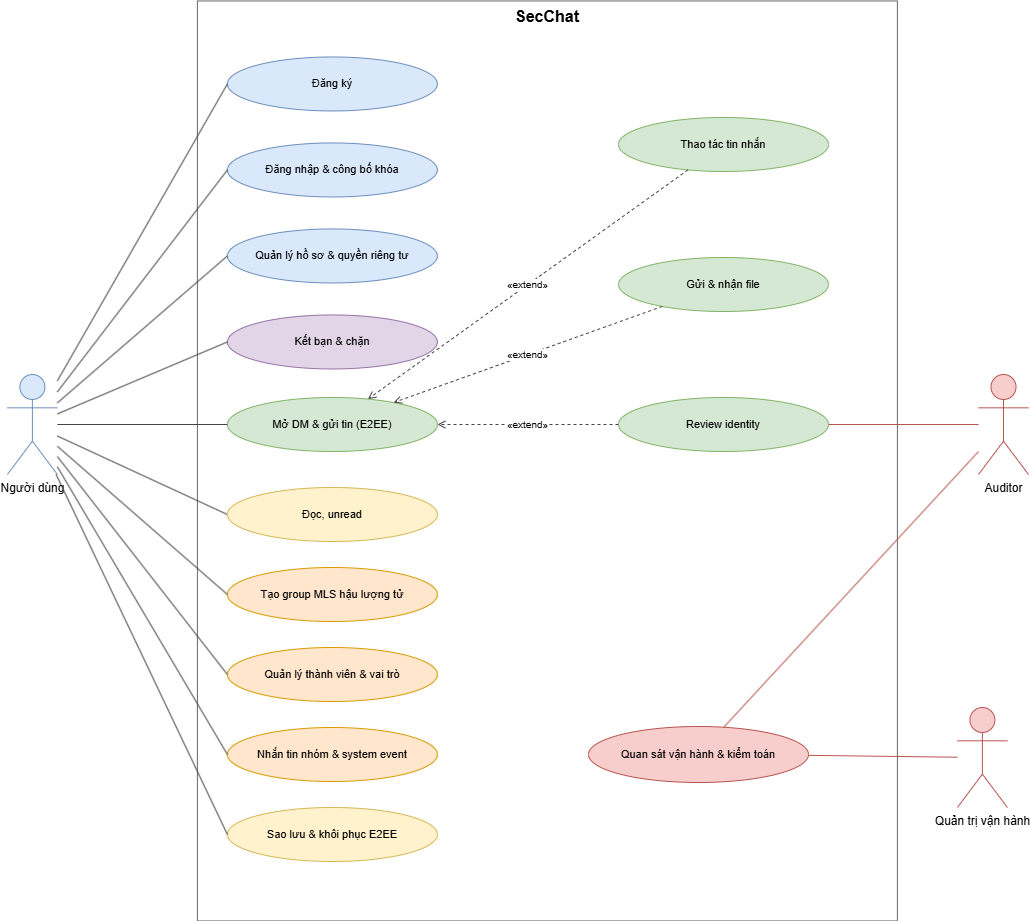
\includegraphics[width=0.95\linewidth]{Figure/UseCaseDiagram.png}
    \caption{Sơ đồ use case tổng quan của SecChat}
    \label{fig:usecase-diagram}
\end{figure}

Các tác nhân tham gia hệ thống gồm:

\begin{itemize}
    \item \textbf{Người dùng:} tác nhân chính của hệ thống. Người dùng thực hiện đăng ký, đăng nhập, kết bạn và chặn, nhắn tin trực tiếp và nhắn tin nhóm được mã hóa đầu cuối, thao tác trên tin nhắn, gửi file, kiểm tra danh tính, quản lý hồ sơ, quyền riêng tư và sao lưu hoặc khôi phục dữ liệu E2EE.
    \item \textbf{Auditor:} dịch vụ minh bạch khóa định danh, hoạt động độc lập với chat server. Auditor đọc log định danh, dựng cây Merkle, ký checkpoint và cấp inclusion proof để client kiểm tra khóa định danh của người khác trước khi tin tưởng.
    \item \textbf{Quản trị vận hành:} người triển khai và giám sát hệ thống qua Docker. Tác nhân này kiểm tra health, readiness, metrics và log qua control plane cùng server GUI, nhưng không có khả năng đọc nội dung tin nhắn của người dùng.
\end{itemize}



\subsection{Đặc tả chức năng}\label{subsec:usecase-spec}

Phần này tóm tắt toàn bộ use case mức hệ thống ở bảng~\ref{tab:usecase-summary}, sau đó đặc tả chi tiết cho bốn use case cốt lõi và phức tạp nhất: đăng nhập và công bố khóa (UC02), mở DM và gửi tin (UC05), quản lý thành viên group MLS (UC10) và sao lưu, khôi phục E2EE (UC13). Các use case còn lại dùng chung cơ chế client gửi lệnh, server kiểm quyền rồi trả event.

\begin{table}[H]
    \centering
    \small
    \begin{tabularx}{\linewidth}{|c|p{0.24\linewidth}|p{0.17\linewidth}|X|}
        \hline
        \textbf{Mã} & \textbf{Use case} & \textbf{Tác nhân} & \textbf{Tóm tắt} \\
        \hline
        UC01 & Đăng ký & Người dùng & Tạo tài khoản, khởi tạo state E2EE và công bố khóa lần đầu. \\ \hline
        UC02 (*) & Đăng nhập và công bố khóa & Người dùng, Auditor & Xác thực, mở local state, công bố PQXDH bundle và MLS KeyPackage. \\ \hline
        UC03 & Quản lý hồ sơ và quyền riêng tư & Người dùng & Cập nhật hồ sơ, avatar, đổi mật khẩu, quyền riêng tư và cache. \\ \hline
        UC04 & Kết bạn và chặn & Người dùng & Tìm, mời, chấp nhận/từ chối kết bạn; chặn/bỏ chặn. \\ \hline
        UC05 (*) & Mở DM và gửi tin & Người dùng, Auditor & Bắt tay PQXDH, gửi \texttt{S3PQI} rồi \texttt{S3DR}; server chỉ lưu ciphertext. \\ \hline
        UC06 & Thao tác tin nhắn & Người dùng & Trả lời, chỉnh sửa, xóa, ghim, thả cảm xúc, chuyển tiếp. \\ \hline
        UC07 & Gửi và nhận file & Người dùng & Mã hóa và gửi tệp đính kèm trong lớp E2EE. \\ \hline
        UC08 & Review identity & Người dùng, Auditor & So sánh safety number qua kênh ngoài, đánh dấu đã xác minh. \\ \hline
        UC09 & Tạo group MLS hậu lượng tử & Người dùng, Server & Tạo group X-Wing, claim KeyPackage; server validate public state. \\ \hline
        UC10 (*) & Quản lý thành viên và vai trò & Admin group & \texttt{prepare}/\texttt{apply}: thêm/xóa/đổi role; server validate \texttt{PublicGroup}. \\ \hline
        UC11 & Nhắn tin nhóm và system event & Thành viên group & Gửi \texttt{S3MLS}; thay đổi membership hiển thị như system event. \\ \hline
        UC12 & Đọc, unread & Người dùng & \texttt{mark\_read} theo message id. \\ \hline
        UC13 (*) & Sao lưu và khôi phục E2EE & Người dùng & Export/restore state mã hóa passphrase; không rollback identity. \\ \hline
        UC14 & Quan sát vận hành và kiểm toán & Quản trị vận hành, Auditor & Kiểm tra health/metrics/log; auditor cấp Merkle proof. \\ \hline
    \end{tabularx}
    \caption{Tổng hợp các use case mức hệ thống ((*): có đặc tả chi tiết bên dưới)}
    \label{tab:usecase-summary}
\end{table}

\subsubsection{UC02 - Đăng nhập và công bố khóa}

\begin{longtable}{|p{0.22\linewidth}|p{0.71\linewidth}|}
\caption{Đặc tả Use Case: Đăng nhập và công bố khóa (UC02)}\label{tab:uc02}\\
\hline
\textbf{Tên Use Case} & Đăng nhập và công bố khóa \\ \hline
\textbf{Tác nhân} & Người dùng (chính), Auditor (phụ) \\ \hline
\textbf{Tiền điều kiện} &
\begin{itemize}
  \item Đã có tài khoản.
  \item Máy hiện tại có local state E2EE, hoặc có backup/identity secret nếu là máy mới.
\end{itemize} \\ \hline
\textbf{Luồng sự kiện chính} &
\begin{enumerate}
  \item Người dùng nhập email và mật khẩu.
  \item Client băm mật khẩu (PBKDF2, salt là email) và gửi gói \texttt{auth}.
  \item Server rate-limit theo (login, IP), xác minh PBKDF2 và đặt trạng thái online.
  \item Client dẫn xuất master key và mở local state đã mã hóa.
  \item Client công bố PQXDH bundle mới cho máy hiện tại và MLS KeyPackage X-Wing.
  \item Server flush notification offline; client tải inbox, danh sách bạn và hội thoại.
\end{enumerate} \\ \hline
\textbf{Luồng sự kiện phát sinh} &
\begin{itemize}
  \item Sai mật khẩu hoặc vượt số lần cho phép: bị khóa tạm thời theo rate limit và báo lỗi.
  \item Máy mới thiếu identity secret: client yêu cầu restore backup hoặc rotate có chủ đích; không tự rotate âm thầm.
\end{itemize} \\ \hline
\textbf{Hậu điều kiện} &
\begin{itemize}
  \item Người dùng online; bundle của máy hiện tại đã được công bố; sẵn sàng gửi và nhận tin.
\end{itemize} \\ \hline
\end{longtable}

\begin{figure}[H]
\centering
\IfFileExists{Figure/ActivityUC02.png}{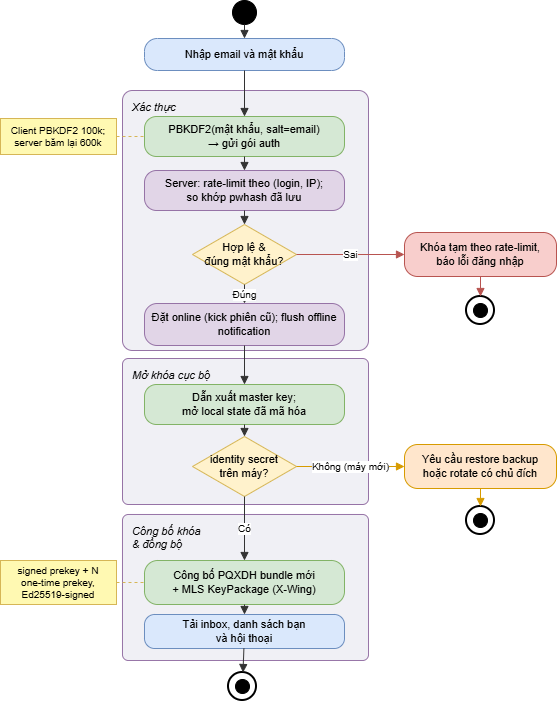
\includegraphics[width=0.72\linewidth]{Figure/ActivityUC02.png}}{\fbox{\parbox[c][3.2cm][c]{0.58\linewidth}{\centering\itshape Sơ đồ hoạt động UC02\\(xuất PNG từ \texttt{diagrams/ActivityUC02.drawio})}}}
\caption{Sơ đồ hoạt động: Đăng nhập và công bố khóa (UC02)}
\label{fig:act-uc02}
\end{figure}

\subsubsection{UC05 - Mở DM và gửi tin}

\begin{longtable}{|p{0.22\linewidth}|p{0.71\linewidth}|}
\caption{Đặc tả Use Case: Mở DM và gửi tin (UC05)}\label{tab:uc05}\\
\hline
\textbf{Tên Use Case} & Mở DM và gửi tin \\ \hline
\textbf{Tác nhân} & Người dùng (chính), Auditor (phụ) \\ \hline
\textbf{Tiền điều kiện} &
\begin{itemize}
  \item Hai bên là bạn hoặc được phép DM; peer đã công bố bundle.
\end{itemize} \\ \hline
\textbf{Luồng sự kiện chính} &
\begin{enumerate}
  \item Client gọi \texttt{start\_dm}; server kiểm tra quyền và chặn tự-DM.
  \item Client gọi \texttt{get\_pqxdh\_bundle}; server trả bundle của peer kèm one-time prekey cùng generation và \texttt{identity\_version}.
  \item Client hỏi auditor lấy Merkle proof cho \texttt{identity\_version} và kiểm tra tính hợp lệ.
  \item Client verify chữ ký prekey, sinh X25519 ephemeral, encapsulate vào ML-KEM của peer, trộn các DH secret và KEM secret bằng HKDF để tạo root secret và khởi tạo Double Ratchet.
  \item Client mã hóa tin đầu tiên và gửi với prefix \texttt{S3PQI}; các tin sau dùng \texttt{S3DR}.
  \item Server lưu ciphertext và chuyển tiếp cho peer; peer giải mã và tiến ratchet.
\end{enumerate} \\ \hline
\textbf{Luồng sự kiện phát sinh} &
\begin{itemize}
  \item Peer thiếu bundle: client báo lỗi rõ và không gửi plaintext.
  \item Bị chặn: server từ chối; bubble đang gửi chuyển sang trạng thái thất bại.
  \item Audit mismatch: hiển thị cảnh báo nhưng vẫn cho gửi (cảnh báo, không chặn).
\end{itemize} \\ \hline
\textbf{Hậu điều kiện} &
\begin{itemize}
  \item Tin được lưu dưới dạng ciphertext; trạng thái ratchet tiến lên.
\end{itemize} \\ \hline
\end{longtable}

\begin{figure}[H]
\centering
\IfFileExists{Figure/ActivityUC05.png}{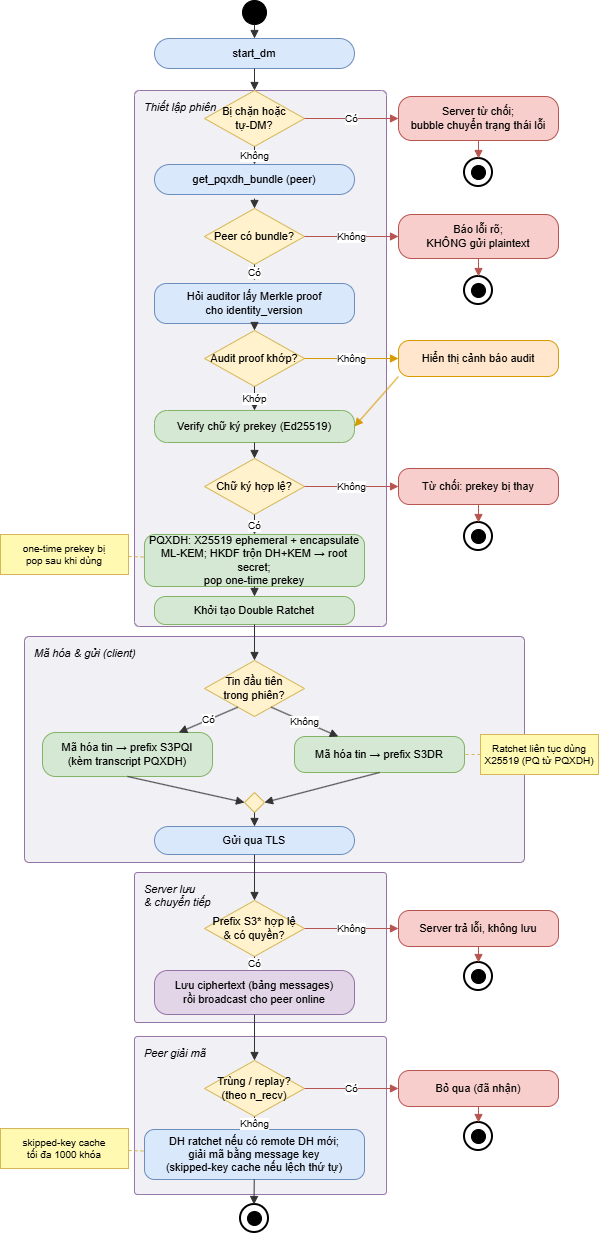
\includegraphics[width=0.72\linewidth]{Figure/ActivityUC05.png}}{\fbox{\parbox[c][3.2cm][c]{0.58\linewidth}{\centering\itshape Sơ đồ hoạt động UC05\\(xuất PNG từ \texttt{diagrams/ActivityUC05.drawio})}}}
\caption{Sơ đồ hoạt động: Mở DM và gửi tin (UC05)}
\label{fig:act-uc05}
\end{figure}

\subsubsection{UC10 - Quản lý thành viên và vai trò}

\begin{longtable}{|p{0.22\linewidth}|p{0.71\linewidth}|}
\caption{Đặc tả Use Case: Quản lý thành viên và vai trò (UC10)}\label{tab:uc10}\\
\hline
\textbf{Tên Use Case} & Quản lý thành viên và vai trò \\ \hline
\textbf{Tác nhân} & Admin group (chính), Server, OpenMLS bridge \\ \hline
\textbf{Tiền điều kiện} &
\begin{itemize}
  \item Là admin (thêm/xóa/đổi role/đổi info) hoặc thành viên (rời nhóm).
\end{itemize} \\ \hline
\textbf{Luồng sự kiện chính} &
\begin{enumerate}
  \item Admin chọn thao tác: thêm/xóa thành viên, đổi role, đổi thông tin nhóm hoặc rời nhóm.
  \item \texttt{prepare\_group\_change}: server kiểm tra policy (quyền admin, friend/block, KeyPackage còn dùng) và tạo operation id.
  \item Client tạo Commit, Welcome và GroupInfo qua OpenMLS.
  \item \texttt{apply\_group\_change}: server validate \texttt{PublicGroup}, đối chiếu member set với pending operation và epoch nối tiếp rồi mutate membership và ghi system event.
\end{enumerate} \\ \hline
\textbf{Luồng sự kiện phát sinh} &
\begin{itemize}
  \item Không phải admin hoặc xóa một admin khác: bị từ chối.
  \item Validation thất bại: handshake không được lưu, membership giữ nguyên.
\end{itemize} \\ \hline
\textbf{Hậu điều kiện} &
\begin{itemize}
  \item Membership và role được cập nhật; system event ghi vào timeline; thành viên bị xóa không nhận epoch mới.
\end{itemize} \\ \hline
\end{longtable}

\begin{figure}[H]
\centering
\IfFileExists{Figure/ActivityUC10.png}{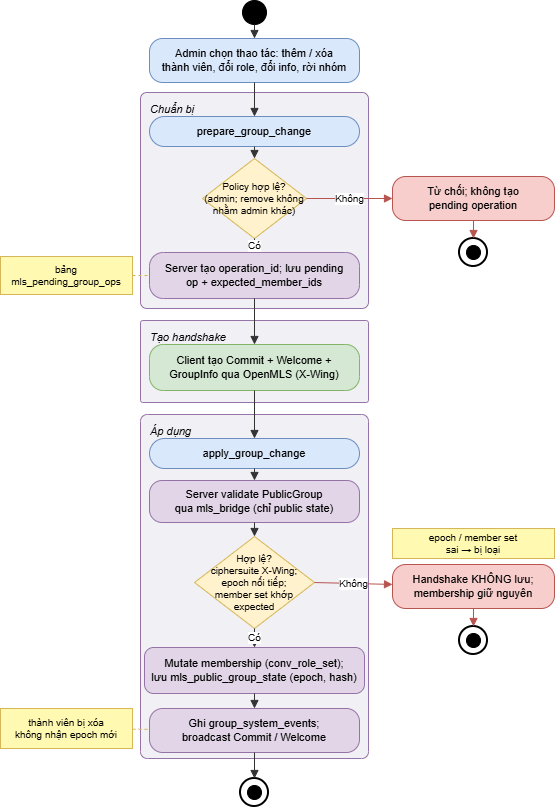
\includegraphics[width=0.72\linewidth]{Figure/ActivityUC10.png}}{\fbox{\parbox[c][3.2cm][c]{0.58\linewidth}{\centering\itshape Sơ đồ hoạt động UC10\\(xuất PNG từ \texttt{diagrams/ActivityUC10.drawio})}}}
\caption{Sơ đồ hoạt động: Quản lý thành viên và vai trò (UC10)}
\label{fig:act-uc10}
\end{figure}

\subsubsection{UC13 - Sao lưu và khôi phục E2EE}

\begin{longtable}{|p{0.22\linewidth}|p{0.71\linewidth}|}
\caption{Đặc tả Use Case: Sao lưu và khôi phục E2EE (UC13)}\label{tab:uc13}\\
\hline
\textbf{Tên Use Case} & Sao lưu và khôi phục E2EE \\ \hline
\textbf{Tác nhân} & Người dùng (chính) \\ \hline
\textbf{Tiền điều kiện} &
\begin{itemize}
  \item Đã đăng nhập (khi sao lưu); có file backup và passphrase (khi khôi phục).
\end{itemize} \\ \hline
\textbf{Luồng sự kiện chính} &
\begin{enumerate}
  \item Người dùng chọn export và chọn có kèm plaintext cache hay không.
  \item Client đóng gói local state (identity, prekey, ratchet, group) và cache tùy chọn, mã hóa bằng PBKDF2(passphrase) cùng AES-GCM với manifest làm AAD.
  \item Khi khôi phục, người dùng mở file, nhập passphrase và client giải mã.
  \item Client re-wrap state bằng master key hiện tại, merge cache theo message id và công bố lại bundle nếu khôi phục được identity secret.
\end{enumerate} \\ \hline
\textbf{Luồng sự kiện phát sinh} &
\begin{itemize}
  \item Sai passphrase: báo lỗi không thể giải mã.
  \item Backup dùng passphrase yếu: bị từ chối.
  \item Khôi phục sau khi đã rotate identity: không rollback identity, chỉ merge cache đọc được.
\end{itemize} \\ \hline
\textbf{Hậu điều kiện} &
\begin{itemize}
  \item Lịch sử đọc được khôi phục cục bộ; server không nhận plaintext.
\end{itemize} \\ \hline
\end{longtable}

\begin{figure}[H]
\centering
\IfFileExists{Figure/ActivityUC13.png}{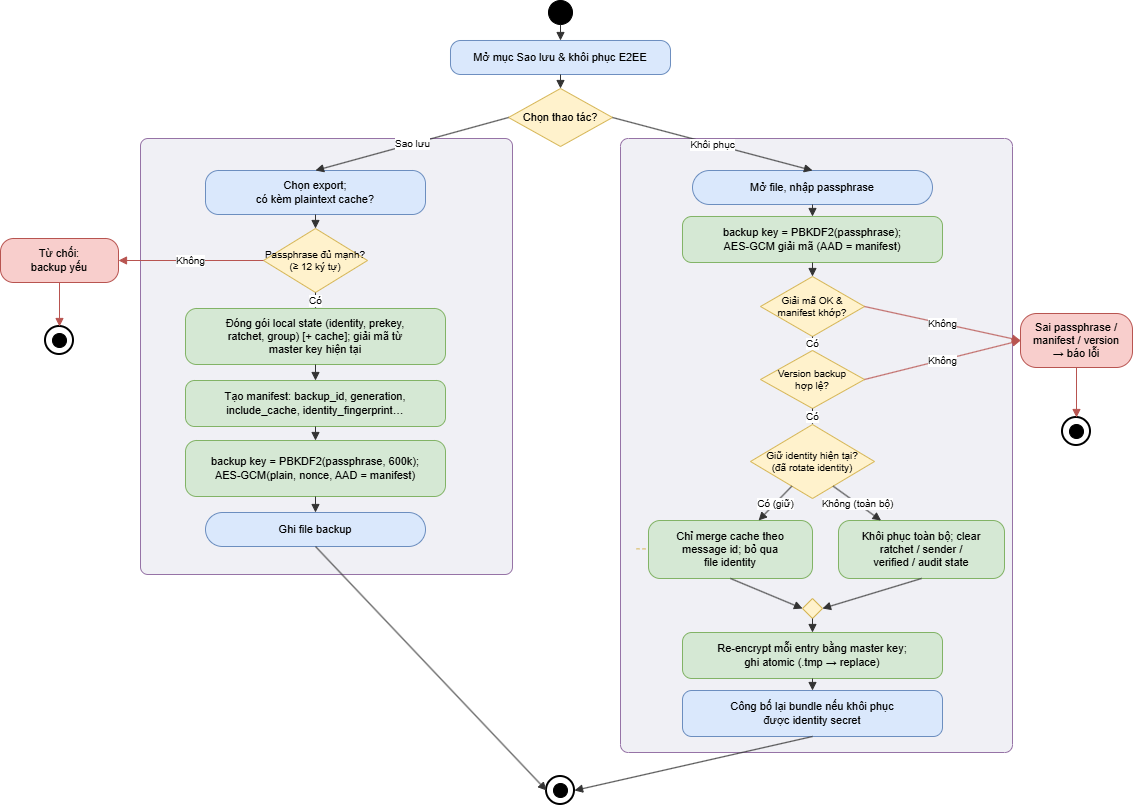
\includegraphics[width=0.98\linewidth]{Figure/ActivityUC13.png}}{\fbox{\parbox[c][3.2cm][c]{0.58\linewidth}{\centering\itshape Sơ đồ hoạt động UC13\\(xuất PNG từ \texttt{diagrams/ActivityUC13.drawio})}}}
\caption{Sơ đồ hoạt động: Sao lưu và khôi phục E2EE (UC13)}
\label{fig:act-uc13}
\end{figure}

\section{Thiết kế hệ thống}

\subsection{Thiết kế cơ sở dữ liệu}

Database của SecChat gồm 20 bảng, không lưu plaintext message, nhưng vẫn lưu metadata cần thiết để hệ thống vận hành. Trường body của bảng \texttt{messages} chỉ chứa ciphertext theo định dạng prefix của giao thức (trình bày ở mục~\ref{subsec:body-format}). Các bảng \texttt{conversation\_members}, \texttt{mls\_group\_state} và \texttt{group\_system\_events} là các điểm quan trọng để bảo đảm group state và timeline ổn định. Các sơ đồ ERD trong mục này là mô hình dữ liệu chính ở mức thiết kế logic. 

\begin{figure}[H]
    \centering
    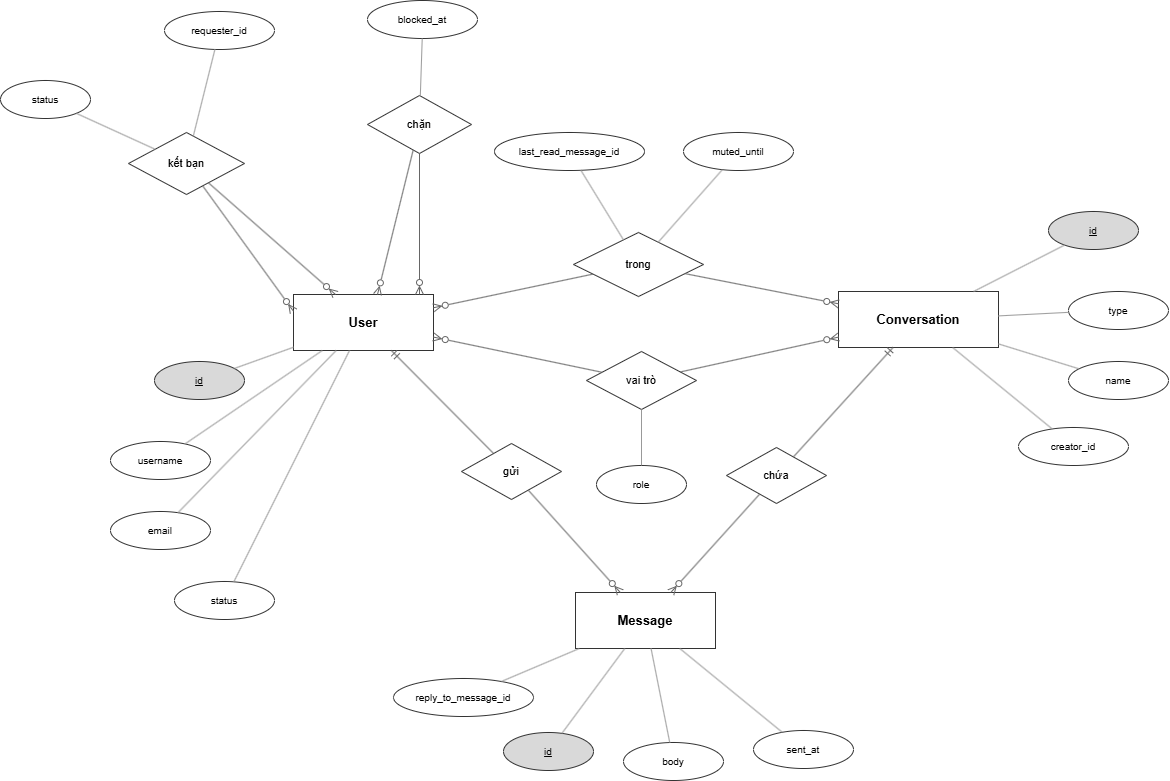
\includegraphics[width=0.96\linewidth]{Figure/ERD_Core.png}
    \caption{ERD phân hệ lõi: người dùng, hội thoại và tin nhắn}
    \label{fig:erd-core}
\end{figure}

\begin{figure}[H]
    \centering
    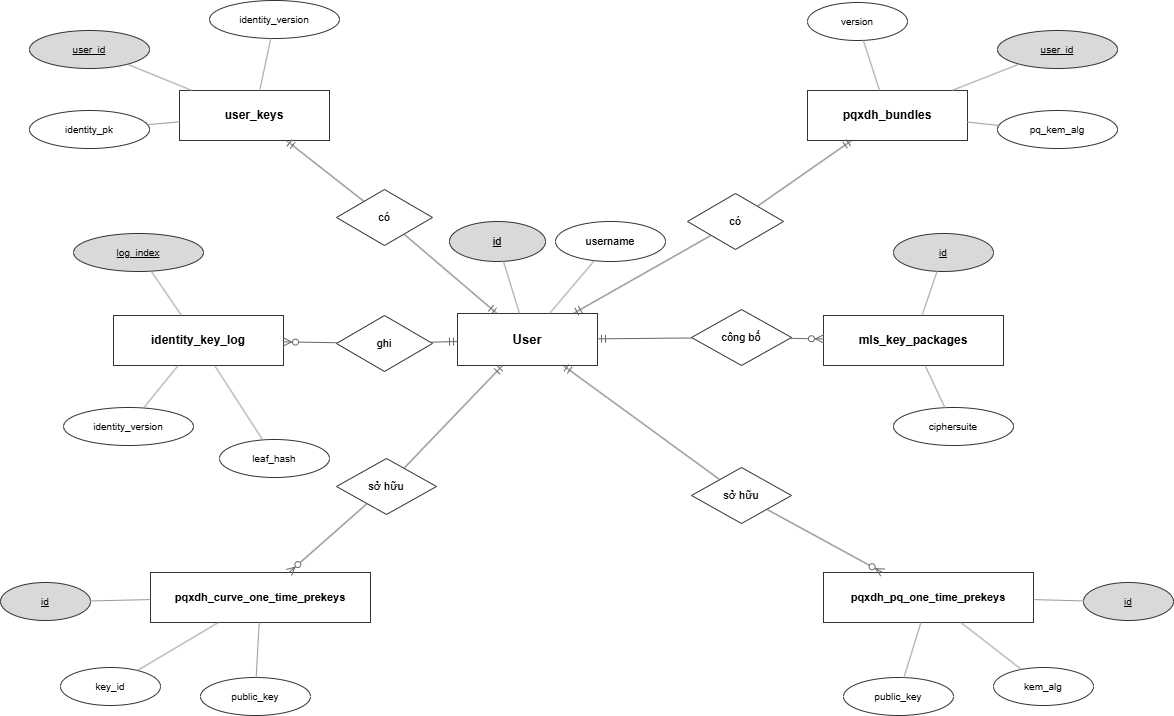
\includegraphics[width=0.96\linewidth]{Figure/ERD_Keys.png}
    \caption{ERD phân hệ khóa và định danh (PQXDH, MLS KeyPackage, identity log)}
    \label{fig:erd-keys}
\end{figure}

\begin{figure}[H]
    \centering
    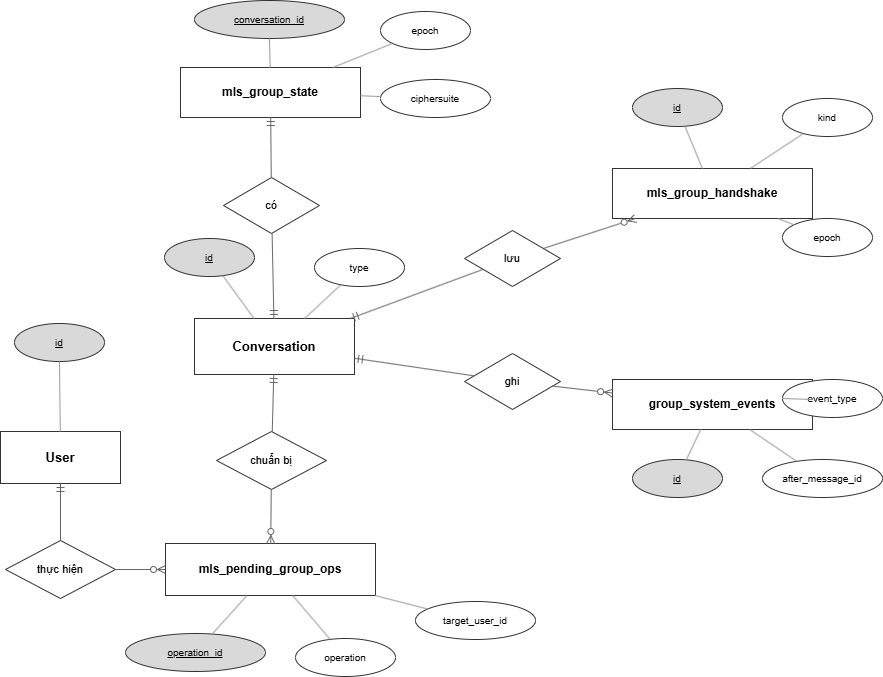
\includegraphics[width=0.92\linewidth]{Figure/ERD_GroupMLS.png}
    \caption{ERD phân hệ nhóm MLS (group state, handshake, system event, pending op)}
    \label{fig:erd-groupmls}
\end{figure}

\begin{figure}[H]
    \centering
    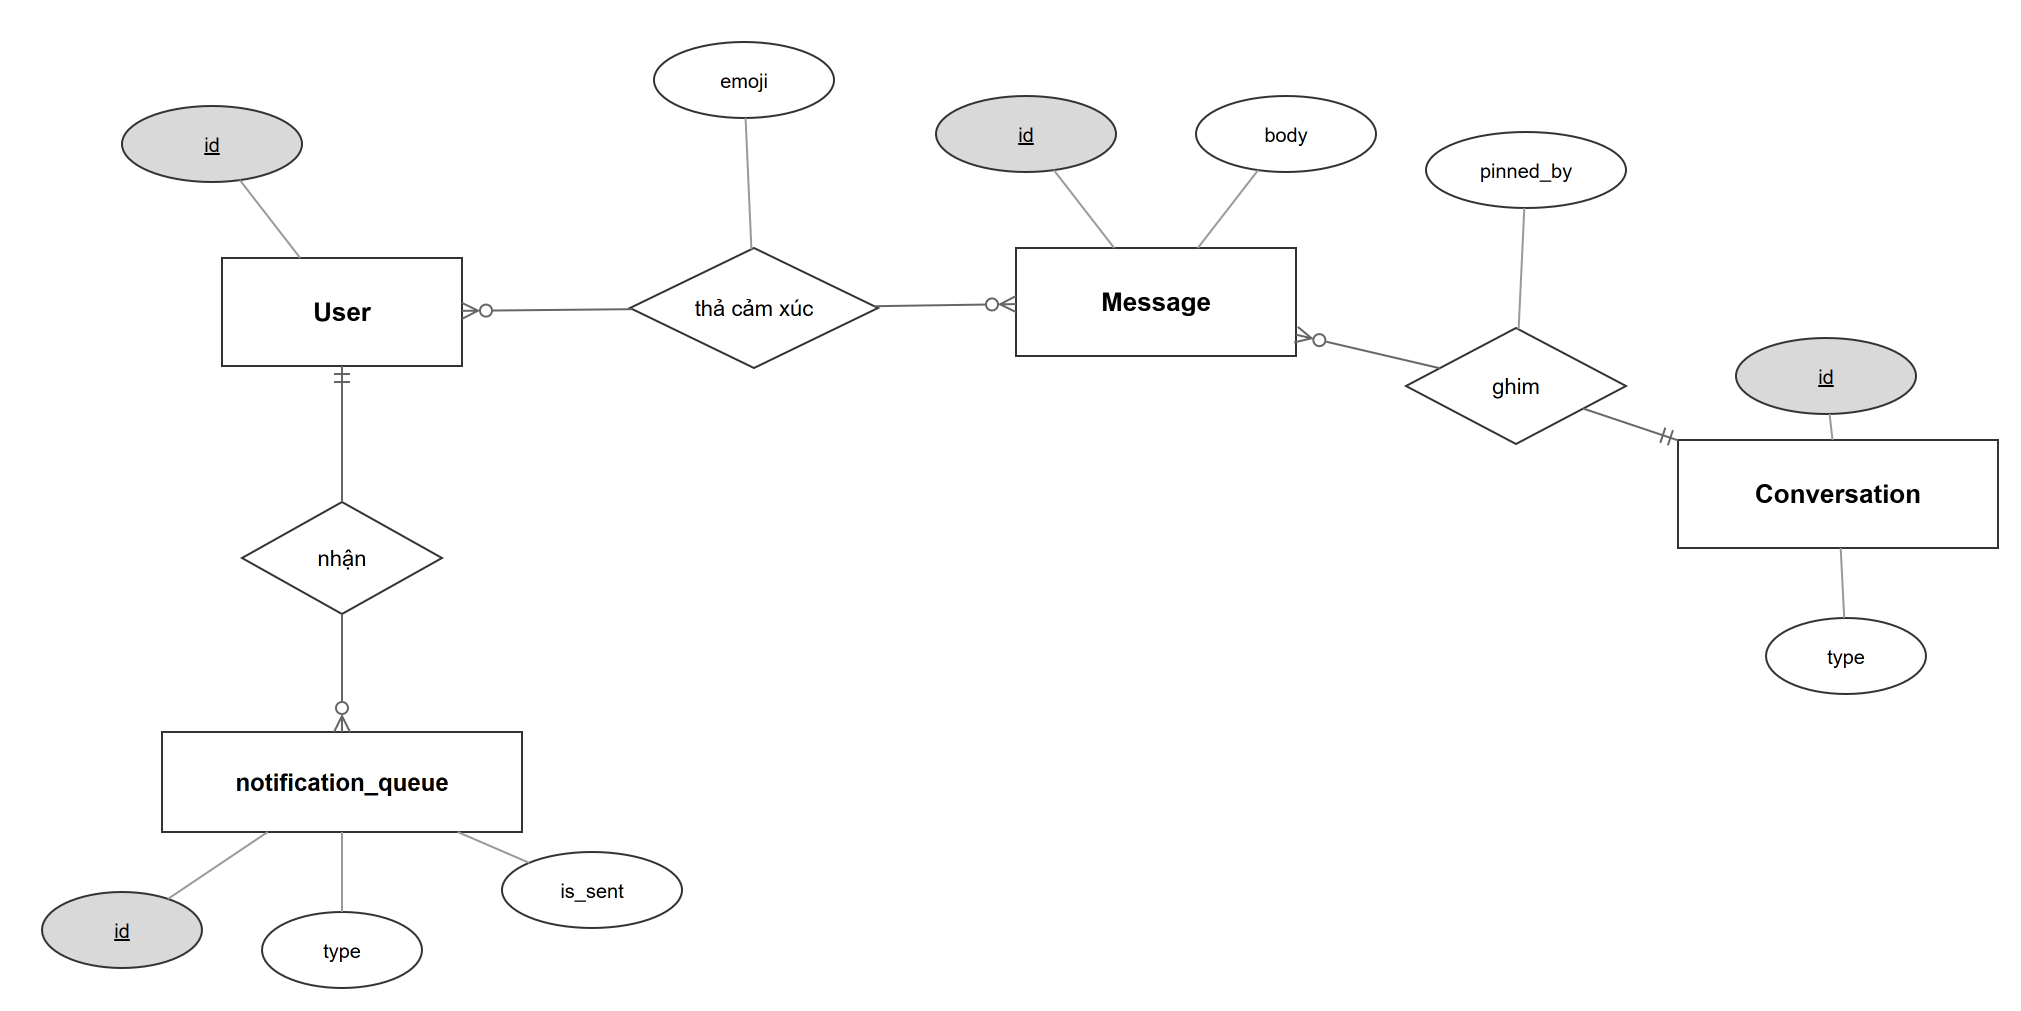
\includegraphics[width=0.96\linewidth]{Figure/ERD_Messaging.png}
    \caption{ERD phân hệ tiện ích tin nhắn và thông báo (reaction, pin, notification)}
    \label{fig:erd-messaging}
\end{figure}

\subsection{Mô tả thực thể}

Bảng mô tả thực thể dưới đây trình bày các thuộc tính chính của từng bảng dữ liệu. Các trường kỹ thuật lặp lại như mốc tạo/cập nhật, cờ trạng thái phụ hoặc dữ liệu phụ trợ chỉ được nêu khi ảnh hưởng trực tiếp đến luồng nghiệp vụ, E2EE, MLS hoặc quan sát vận hành.

{\footnotesize
\begin{longtable}{|p{0.23\linewidth}|p{0.25\linewidth}|p{0.16\linewidth}|p{0.24\linewidth}|}
\caption{Mô tả các thực thể dữ liệu chính}\label{tab:entity-detail}\\
\hline
\textbf{Thực thể} & \textbf{Tên thuộc tính} & \textbf{Kiểu dữ liệu} & \textbf{Mô tả} \\ \hline
\endfirsthead
\hline
\textbf{Thực thể} & \textbf{Tên thuộc tính} & \textbf{Kiểu dữ liệu} & \textbf{Mô tả} \\ \hline
\endhead
\texttt{users} & \texttt{id} & INT, PK & Khóa chính tự tăng. \\ \cline{2-4}
 & \texttt{username} & VARCHAR(64), UNIQUE & Tên đăng nhập. \\ \cline{2-4}
 & \texttt{email} & VARCHAR(200) & Email đăng nhập. \\ \cline{2-4}
 & \texttt{password\_hash} & VARCHAR(200) & Hash mật khẩu (PBKDF2 salt server), không lưu plaintext. \\ \cline{2-4}
 & \texttt{display\_name} & VARCHAR(100) & Tên hiển thị. \\ \cline{2-4}
 & \texttt{avatar} & MEDIUMBLOB & Ảnh đại diện (kèm \texttt{avatar\_mime}). \\ \cline{2-4}
 & \texttt{status} & ENUM (online /offline /away) & Trạng thái hiện diện. \\ \cline{2-4}
 & \texttt{privacy\_online}, \texttt{privacy\_last\_seen} & ENUM (everyone /friends /nobody) & Quyền riêng tư hiện diện. \\ \hline
\texttt{friendships} & \texttt{id} & BIGINT, PK & Khóa chính. \\ \cline{2-4}
 & \texttt{user\_id}, \texttt{friend\_id} & INT, FK & Cặp người dùng trong quan hệ. \\ \cline{2-4}
 & \texttt{requester\_id} & INT, FK & Người gửi lời mời. \\ \cline{2-4}
 & \texttt{status} & ENUM (pending /accepted /blocked) & Trạng thái quan hệ. \\ \hline
\texttt{user\_blocks} & \texttt{blocker\_id} & INT, PK, FK & Người chặn. \\ \cline{2-4}
 & \texttt{blocked\_id} & INT, PK, FK & Người bị chặn. \\ \cline{2-4}
 & \texttt{blocked\_at} & DATETIME & Thời điểm chặn. \\ \hline
\texttt{conversations} & \texttt{id} & BIGINT, PK & Khóa chính. \\ \cline{2-4}
 & \texttt{type} & ENUM (direct /group) & Loại hội thoại. \\ \cline{2-4}
 & \texttt{name} & VARCHAR(100) & Tên nhóm. \\ \cline{2-4}
 & \texttt{creator\_id} & INT, FK & Người tạo nhóm. \\ \cline{2-4}
 & \texttt{description} & TEXT & Mô tả nhóm (kèm \texttt{avatar}). \\ \cline{2-4}
 & \texttt{disappear\_after\_secs} & INT & Thời gian tin tự hủy (kèm \texttt{disappear\_enabled\_at}). \\ \cline{2-4}
 & \texttt{is\_disbanded} & TINYINT(1) & Cờ nhóm đã giải tán. \\ \hline
\texttt{conversation\_members} & \texttt{id} & BIGINT, PK & Khóa chính. \\ \cline{2-4}
 & \texttt{conversation\_id} & BIGINT, FK & Hội thoại. \\ \cline{2-4}
 & \texttt{user\_id} & INT, FK & Thành viên. \\ \cline{2-4}
 & \texttt{last\_read\_message\_id} & BIGINT & Con trỏ đã đọc. \\ \cline{2-4}
 & \texttt{force\_unread} & TINYINT & Đánh dấu chưa đọc thủ công. \\ \cline{2-4}
 & \texttt{muted\_until}, \texttt{conv\_pinned\_at} & DATETIME & Tắt thông báo / ghim hội thoại. \\ \hline
\texttt{group\_roles} & \texttt{conversation\_id} & BIGINT, PK, FK & Nhóm. \\ \cline{2-4}
 & \texttt{user\_id} & INT, PK, FK & Thành viên. \\ \cline{2-4}
 & \texttt{role} & ENUM (admin /member) & Vai trò trong nhóm. \\ \hline
\texttt{messages} & \texttt{id} & BIGINT, PK & Khóa chính. \\ \cline{2-4}
 & \texttt{conversation\_id} & BIGINT, FK & Hội thoại. \\ \cline{2-4}
 & \texttt{sender\_id} & INT, FK & Người gửi. \\ \cline{2-4}
 & \texttt{body} & LONGTEXT & Ciphertext, prefix \texttt{S3PQI}/\texttt{S3DR}/\texttt{S3MLS} (tệp đính kèm là marker \texttt{FILE:} bên trong plaintext đã giải mã). \\ \cline{2-4}
 & \texttt{reply\_to\_message\_id} & BIGINT & Tin được trả lời. \\ \cline{2-4}
 & \texttt{edit\_target\_message\_id} & BIGINT & Tin gốc của event chỉnh sửa. \\ \cline{2-4}
 & \texttt{deleted\_at} & DATETIME(3) & Mốc soft-delete. \\ \hline
\texttt{message\_reactions} & \texttt{id} & BIGINT, PK & Khóa chính. \\ \cline{2-4}
 & \texttt{message\_id} & BIGINT, FK & Tin được thả cảm xúc. \\ \cline{2-4}
 & \texttt{user\_id} & INT, FK & Người thả. \\ \cline{2-4}
 & \texttt{emoji} & VARCHAR(16) & Biểu tượng cảm xúc. \\ \hline
\texttt{pinned\_messages} & \texttt{conversation\_id} & BIGINT, PK, FK & Hội thoại. \\ \cline{2-4}
 & \texttt{message\_id} & BIGINT, PK, FK & Tin được ghim. \\ \cline{2-4}
 & \texttt{pinned\_by} & INT, FK & Người ghim. \\ \hline
\texttt{user\_keys} & \texttt{user\_id} & INT, PK, FK & Chủ sở hữu khóa. \\ \cline{2-4}
 & \texttt{identity\_pk} & TEXT & Ed25519 identity public key. \\ \cline{2-4}
 & \texttt{identity\_sig} & TEXT & Chữ ký tự xác thực identity. \\ \cline{2-4}
 & \texttt{identity\_sk\_enc} & TEXT & Identity secret đã mã hóa bằng master key. \\ \cline{2-4}
 & \texttt{identity\_version} & INT & Phiên bản identity. \\ \hline
\texttt{pqxdh\_bundles} & \texttt{user\_id} & INT, PK, FK & Chủ bundle. \\ \cline{2-4}
 & \texttt{curve\_spk}, \texttt{curve\_spk\_sig} & TEXT & Signed X25519 prekey và chữ ký. \\ \cline{2-4}
 & \texttt{pq\_kem\_alg} & VARCHAR(32) & Tên thuật toán KEM đang dùng (ví dụ \texttt{ML-KEM-1024}). \\ \cline{2-4}
 & \texttt{pq\_spk}, \texttt{pq\_spk\_sig} & TEXT & Signed PQ KEM prekey và chữ ký. \\ \cline{2-4}
 & \texttt{version} & INT & Phiên bản bundle. \\ \hline
\makecell[tl]{\texttt{pqxdh\_curve\_}\\\texttt{one\_time\_prekeys}} & \texttt{id} & BIGINT, PK & Khóa chính. \\ \cline{2-4}
 & \texttt{user\_id} & INT, FK & Chủ prekey. \\ \cline{2-4}
 & \texttt{key\_id} & INT & Định danh prekey. \\ \cline{2-4}
 & \texttt{public\_key}, \texttt{signature} & TEXT & One-time X25519 prekey và chữ ký. \\ \hline
\makecell[tl]{\texttt{pqxdh\_pq\_}\\\texttt{one\_time\_prekeys}} & \texttt{id} & BIGINT, PK & Khóa chính. \\ \cline{2-4}
 & \texttt{user\_id} & INT, FK & Chủ prekey. \\ \cline{2-4}
 & \texttt{kem\_alg} & VARCHAR(32) & Thuật toán KEM. \\ \cline{2-4}
 & \texttt{public\_key}, \texttt{signature} & TEXT & One-time PQ KEM prekey và chữ ký. \\ \hline
\texttt{identity\_key\_log} & \texttt{log\_index} & BIGINT, PK & Chỉ số append-only. \\ \cline{2-4}
 & \texttt{user\_id} & INT, FK & Chủ identity. \\ \cline{2-4}
 & \texttt{identity\_version} & INT & Phiên bản identity. \\ \cline{2-4}
 & \texttt{identity\_pk} & TEXT & Identity key tại version đó. \\ \cline{2-4}
 & \texttt{event\_type} & ENUM (initial /rotation) & Loại sự kiện. \\ \cline{2-4}
 & \texttt{leaf\_hash} & CHAR(64) & Hash lá Merkle. \\ \hline
\texttt{mls\_key\_packages} & \texttt{id} & BIGINT, PK & Khóa chính. \\ \cline{2-4}
 & \texttt{user\_id} & INT, FK & Chủ KeyPackage. \\ \cline{2-4}
 & \texttt{ciphersuite} & VARCHAR(128) & Ciphersuite X-Wing. \\ \cline{2-4}
 & \texttt{key\_package\_b64} & LONGTEXT & KeyPackage MLS (base64). \\ \cline{2-4}
 & \texttt{secchat\_signature} & TEXT & Chữ ký SecChat trên KeyPackage. \\ \cline{2-4}
 & \texttt{claimed\_at}, \texttt{claimed\_by} & DATETIME(3), INT & Trạng thái đã claim (single-use). \\ \hline
\texttt{mls\_group\_state} & \texttt{conversation\_id} & BIGINT, PK, FK & Nhóm. \\ \cline{2-4}
 & \texttt{group\_id\_b64} & VARCHAR(256) & Group id MLS. \\ \cline{2-4}
 & \texttt{epoch} & BIGINT & Epoch hiện hành. \\ \cline{2-4}
 & \texttt{ciphersuite} & VARCHAR(128) & Ciphersuite X-Wing. \\ \cline{2-4}
 & \texttt{public\_state\_b64} & LONGTEXT & Public group state đã validate. \\ \cline{2-4}
 & \texttt{public\_state\_hash}, \texttt{validated\_at} & VARCHAR(128), DATETIME(3) & Hash và mốc validate. \\ \hline
\texttt{mls\_pending\_group\_ops} & \texttt{operation\_id} & VARCHAR(64), PK & Định danh operation. \\ \cline{2-4}
 & \texttt{conversation\_id} & BIGINT, FK & Nhóm. \\ \cline{2-4}
 & \texttt{actor\_id} & INT, FK & Người thực hiện. \\ \cline{2-4}
 & \texttt{operation} & VARCHAR(32) & Loại thao tác (add/remove/...). \\ \cline{2-4}
 & \texttt{target\_user\_id} & INT & Đối tượng tác động. \\ \cline{2-4}
 & \texttt{status} & ENUM (prepared /applied /rejected) & Trạng thái; \texttt{expires\_at} giới hạn thời gian. \\ \hline
\texttt{mls\_group\_handshake} & \texttt{id} & BIGINT, PK & Khóa chính. \\ \cline{2-4}
 & \texttt{conversation\_id} & BIGINT, FK & Nhóm. \\ \cline{2-4}
 & \texttt{kind} & ENUM (welcome /commit /group\_info /control) & Loại artifact MLS. \\ \cline{2-4}
 & \texttt{epoch} & BIGINT & Epoch của artifact. \\ \cline{2-4}
 & \texttt{operation\_id} & VARCHAR(64) & Operation liên quan. \\ \cline{2-4}
 & \texttt{mls\_message\_b64} & LONGTEXT & Bytes MLS (base64) để client replay. \\ \hline
\texttt{group\_system\_events} & \texttt{id} & BIGINT, PK & Khóa chính. \\ \cline{2-4}
 & \texttt{conversation\_id} & BIGINT, FK & Nhóm. \\ \cline{2-4}
 & \texttt{event\_type} & VARCHAR(32) & Loại sự kiện (add/remove/role/...). \\ \cline{2-4}
 & \texttt{target\_user\_id}, \texttt{role} & INT, VARCHAR(16) & Đối tượng và vai trò. \\ \cline{2-4}
 & \texttt{operation\_id} & VARCHAR(64) & Khử trùng lặp với realtime. \\ \cline{2-4}
 & \texttt{after\_message\_id} & BIGINT & Vị trí trong timeline. \\ \hline
\texttt{notification\_queue} & \texttt{id} & BIGINT, PK & Khóa chính. \\ \cline{2-4}
 & \texttt{user\_id} & INT, FK & Người nhận. \\ \cline{2-4}
 & \texttt{type} & VARCHAR(64) & Loại notification. \\ \cline{2-4}
 & \texttt{payload} & TEXT & Nội dung sự kiện. \\ \cline{2-4}
 & \texttt{is\_sent} & TINYINT & Đã flush hay chưa. \\ \hline
\end{longtable}
}

\subsection{Thiết kế cấu trúc đối tượng}

Sơ đồ class diagram trong mục này mô tả các lớp và module chính của hệ thống ở mức thiết kế. Mỗi lớp chỉ nêu các thuộc tính và phương thức tiêu biểu thể hiện trách nhiệm của thành phần đó.

\begin{figure}[H]
    \centering
    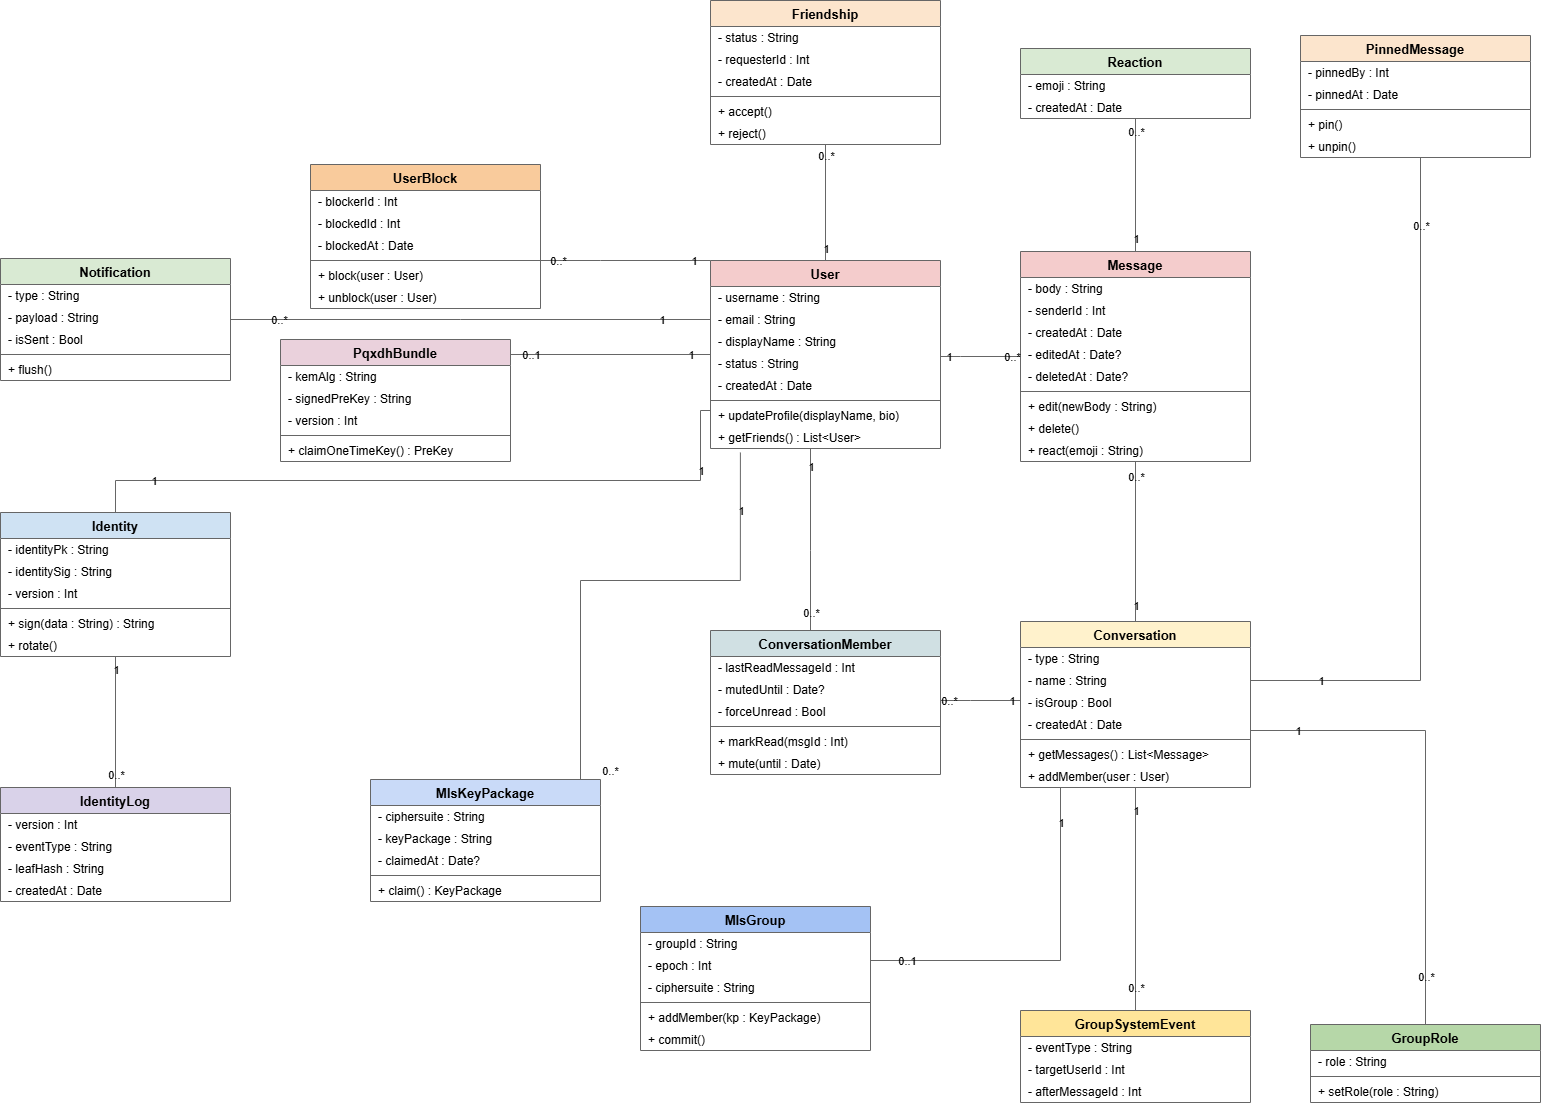
\includegraphics[width=0.98\linewidth]{Figure/ClassDiagramCore.png}
    \caption{Sơ đồ class diagram các lớp chính của hệ thống}
    \label{fig:class-detail}
\end{figure}

\textbf{1. Class: User}

{\small
\begin{longtable}{|p{0.25\linewidth}|p{0.14\linewidth}|p{0.28\linewidth}|p{0.21\linewidth}|}
\hline
\textbf{Tên} & \textbf{Loại} & \textbf{Kiểu dữ liệu / Tham số} & \textbf{Mô tả} \\ \hline
\endhead
\texttt{username} & Thuộc tính & String & Tên đăng nhập (duy nhất). \\ \hline
\texttt{email} & Thuộc tính & String & Email đăng nhập. \\ \hline
\texttt{displayName} & Thuộc tính & String & Tên hiển thị. \\ \hline
\texttt{status} & Thuộc tính & String & Trạng thái hiện diện (online/offline). \\ \hline
\texttt{createdAt} & Thuộc tính & Date & Ngày tạo tài khoản. \\ \hline
\texttt{updateProfile} & Phương thức & displayName, bio & Cập nhật hồ sơ. \\ \hline
\texttt{getFriends} & Phương thức & $\rightarrow$ List\textless User\textgreater  & Lấy danh sách bạn bè. \\ \hline
\end{longtable}
}

\textbf{2. Class: Friendship}

{\small
\begin{longtable}{|p{0.25\linewidth}|p{0.14\linewidth}|p{0.28\linewidth}|p{0.21\linewidth}|}
\hline
\textbf{Tên} & \textbf{Loại} & \textbf{Kiểu dữ liệu / Tham số} & \textbf{Mô tả} \\ \hline
\endhead
\texttt{status} & Thuộc tính & String & Trạng thái (pending/accepted/ blocked). \\ \hline
\texttt{requesterId} & Thuộc tính & Int & Người gửi lời mời. \\ \hline
\texttt{createdAt} & Thuộc tính & Date & Thời điểm tạo. \\ \hline
\texttt{accept} & Phương thức & void & Chấp nhận lời mời. \\ \hline
\texttt{reject} & Phương thức & void & Từ chối lời mời. \\ \hline
\end{longtable}
}

\textbf{3. Class: UserBlock}

{\small
\begin{longtable}{|p{0.25\linewidth}|p{0.14\linewidth}|p{0.28\linewidth}|p{0.21\linewidth}|}
\hline
\textbf{Tên} & \textbf{Loại} & \textbf{Kiểu dữ liệu / Tham số} & \textbf{Mô tả} \\ \hline
\endhead
\texttt{blockerId} & Thuộc tính & Int & Người chặn. \\ \hline
\texttt{blockedId} & Thuộc tính & Int & Người bị chặn. \\ \hline
\texttt{blockedAt} & Thuộc tính & Date & Thời điểm chặn. \\ \hline
\texttt{block} & Phương thức & user: User & Chặn một người dùng. \\ \hline
\texttt{unblock} & Phương thức & user: User & Bỏ chặn. \\ \hline
\end{longtable}
}

\textbf{4. Class: Notification}

{\small
\begin{longtable}{|p{0.25\linewidth}|p{0.14\linewidth}|p{0.28\linewidth}|p{0.21\linewidth}|}
\hline
\textbf{Tên} & \textbf{Loại} & \textbf{Kiểu dữ liệu / Tham số} & \textbf{Mô tả} \\ \hline
\endhead
\texttt{type} & Thuộc tính & String & Loại thông báo. \\ \hline
\texttt{payload} & Thuộc tính & String & Nội dung sự kiện. \\ \hline
\texttt{isSent} & Thuộc tính & Bool & Đã đẩy tới client hay chưa. \\ \hline
\texttt{flush} & Phương thức & void & Đẩy thông báo còn tồn khi user online. \\ \hline
\end{longtable}
}

\textbf{5. Class: IdentityLog}

{\small
\begin{longtable}{|p{0.25\linewidth}|p{0.14\linewidth}|p{0.28\linewidth}|p{0.21\linewidth}|}
\hline
\textbf{Tên} & \textbf{Loại} & \textbf{Kiểu dữ liệu / Tham số} & \textbf{Mô tả} \\ \hline
\endhead
\texttt{version} & Thuộc tính & Int & Phiên bản identity tại sự kiện. \\ \hline
\texttt{eventType} & Thuộc tính & String & Loại sự kiện (initial/rotation). \\ \hline
\texttt{leafHash} & Thuộc tính & String & Hash lá trong cây Merkle minh bạch. \\ \hline
\texttt{createdAt} & Thuộc tính & Date & Thời điểm ghi log. \\ \hline
\end{longtable}
}

\textbf{6. Class: Identity}

{\small
\begin{longtable}{|p{0.25\linewidth}|p{0.14\linewidth}|p{0.28\linewidth}|p{0.21\linewidth}|}
\hline
\textbf{Tên} & \textbf{Loại} & \textbf{Kiểu dữ liệu / Tham số} & \textbf{Mô tả} \\ \hline
\endhead
\texttt{identityPk} & Thuộc tính & String & Khóa định danh công khai Ed25519. \\ \hline
\texttt{identitySig} & Thuộc tính & String & Chữ ký tự xác thực. \\ \hline
\texttt{version} & Thuộc tính & Int & Phiên bản identity. \\ \hline
\texttt{sign} & Phương thức & data: String $\rightarrow$ String & Ký prekey/dữ liệu. \\ \hline
\texttt{rotate} & Phương thức & void & Xoay sang identity key mới. \\ \hline
\end{longtable}
}

\textbf{7. Class: PqxdhBundle}

{\small
\begin{longtable}{|p{0.25\linewidth}|p{0.14\linewidth}|p{0.28\linewidth}|p{0.21\linewidth}|}
\hline
\textbf{Tên} & \textbf{Loại} & \textbf{Kiểu dữ liệu / Tham số} & \textbf{Mô tả} \\ \hline
\endhead
\texttt{kemAlg} & Thuộc tính & String & Thuật toán KEM (ML-KEM-1024). \\ \hline
\texttt{signedPreKey} & Thuộc tính & String & Signed prekey đã ký. \\ \hline
\texttt{version} & Thuộc tính & Int & Phiên bản bundle. \\ \hline
\texttt{claimOneTimeKey} & Phương thức & $\rightarrow$ PreKey & Cấp một one-time prekey. \\ \hline
\end{longtable}
}

\textbf{8. Class: MlsKeyPackage}

{\small
\begin{longtable}{|p{0.25\linewidth}|p{0.14\linewidth}|p{0.28\linewidth}|p{0.21\linewidth}|}
\hline
\textbf{Tên} & \textbf{Loại} & \textbf{Kiểu dữ liệu / Tham số} & \textbf{Mô tả} \\ \hline
\endhead
\texttt{ciphersuite} & Thuộc tính & String & Ciphersuite X-Wing. \\ \hline
\texttt{keyPackage} & Thuộc tính & String & KeyPackage MLS (base64). \\ \hline
\texttt{claimedAt} & Thuộc tính & Date? & Thời điểm bị claim (single-use). \\ \hline
\texttt{claim} & Phương thức & $\rightarrow$ KeyPackage & Lấy KeyPackage để thêm vào nhóm. \\ \hline
\end{longtable}
}

\textbf{9. Class: Conversation}

{\small
\begin{longtable}{|p{0.25\linewidth}|p{0.14\linewidth}|p{0.28\linewidth}|p{0.21\linewidth}|}
\hline
\textbf{Tên} & \textbf{Loại} & \textbf{Kiểu dữ liệu / Tham số} & \textbf{Mô tả} \\ \hline
\endhead
\texttt{type} & Thuộc tính & String & Loại (direct/group). \\ \hline
\texttt{name} & Thuộc tính & String & Tên nhóm. \\ \hline
\texttt{isGroup} & Thuộc tính & Bool & Cờ nhóm/DM. \\ \hline
\texttt{createdAt} & Thuộc tính & Date & Ngày tạo. \\ \hline
\texttt{getMessages} & Phương thức & $\rightarrow$ List\textless Message\textgreater  & Lấy danh sách tin. \\ \hline
\texttt{addMember} & Phương thức & user: User & Thêm thành viên. \\ \hline
\end{longtable}
}

\textbf{10. Class: ConversationMember}

{\small
\begin{longtable}{|p{0.25\linewidth}|p{0.14\linewidth}|p{0.28\linewidth}|p{0.21\linewidth}|}
\hline
\textbf{Tên} & \textbf{Loại} & \textbf{Kiểu dữ liệu / Tham số} & \textbf{Mô tả} \\ \hline
\endhead
\texttt{lastReadMessageId} & Thuộc tính & Int & Con trỏ đã đọc. \\ \hline
\texttt{mutedUntil} & Thuộc tính & Date? & Tắt thông báo đến thời điểm. \\ \hline
\texttt{forceUnread} & Thuộc tính & Bool & Đánh dấu chưa đọc thủ công. \\ \hline
\texttt{markRead} & Phương thức & msgId: Int & Đánh dấu đã đọc tới msgId. \\ \hline
\texttt{mute} & Phương thức & until: Date & Tắt thông báo hội thoại. \\ \hline
\end{longtable}
}

\textbf{11. Class: GroupRole}

{\small
\begin{longtable}{|p{0.25\linewidth}|p{0.14\linewidth}|p{0.28\linewidth}|p{0.21\linewidth}|}
\hline
\textbf{Tên} & \textbf{Loại} & \textbf{Kiểu dữ liệu / Tham số} & \textbf{Mô tả} \\ \hline
\endhead
\texttt{role} & Thuộc tính & String & Vai trò (admin/member). \\ \hline
\texttt{setRole} & Phương thức & role: String & Đặt vai trò thành viên. \\ \hline
\end{longtable}
}

\textbf{12. Class: MlsGroup}

{\small
\begin{longtable}{|p{0.25\linewidth}|p{0.14\linewidth}|p{0.28\linewidth}|p{0.21\linewidth}|}
\hline
\textbf{Tên} & \textbf{Loại} & \textbf{Kiểu dữ liệu / Tham số} & \textbf{Mô tả} \\ \hline
\endhead
\texttt{groupId} & Thuộc tính & String & Định danh group MLS. \\ \hline
\texttt{epoch} & Thuộc tính & Int & Epoch hiện hành. \\ \hline
\texttt{ciphersuite} & Thuộc tính & String & X-Wing (ML-KEM-768 + X25519). \\ \hline
\texttt{addMember} & Phương thức & kp: KeyPackage & Thêm thành viên, sinh Commit/Welcome. \\ \hline
\texttt{commit} & Phương thức & void & Áp thay đổi, tiến epoch. \\ \hline
\end{longtable}
}

\textbf{13. Class: Message}

{\small
\begin{longtable}{|p{0.25\linewidth}|p{0.14\linewidth}|p{0.28\linewidth}|p{0.21\linewidth}|}
\hline
\textbf{Tên} & \textbf{Loại} & \textbf{Kiểu dữ liệu / Tham số} & \textbf{Mô tả} \\ \hline
\endhead
\texttt{body} & Thuộc tính & String & Nội dung đã mã hóa (ciphertext). \\ \hline
\texttt{senderId} & Thuộc tính & Int & Người gửi. \\ \hline
\texttt{createdAt} & Thuộc tính & Date & Thời điểm gửi. \\ \hline
\texttt{editedAt} & Thuộc tính & Date? & Thời điểm sửa (null nếu chưa). \\ \hline
\texttt{deletedAt} & Thuộc tính & Date? & Thời điểm thu hồi (null nếu chưa). \\ \hline
\texttt{edit} & Phương thức & newBody: String & Sửa nội dung. \\ \hline
\texttt{delete} & Phương thức & void & Thu hồi (soft-delete). \\ \hline
\texttt{react} & Phương thức & emoji: String & Thả cảm xúc. \\ \hline
\end{longtable}
}

\textbf{14. Class: Reaction}

{\small
\begin{longtable}{|p{0.25\linewidth}|p{0.14\linewidth}|p{0.28\linewidth}|p{0.21\linewidth}|}
\hline
\textbf{Tên} & \textbf{Loại} & \textbf{Kiểu dữ liệu / Tham số} & \textbf{Mô tả} \\ \hline
\endhead
\texttt{emoji} & Thuộc tính & String & Biểu tượng cảm xúc. \\ \hline
\texttt{createdAt} & Thuộc tính & Date & Thời điểm thả. \\ \hline
\end{longtable}
}

\textbf{15. Class: PinnedMessage}

{\small
\begin{longtable}{|p{0.25\linewidth}|p{0.14\linewidth}|p{0.28\linewidth}|p{0.21\linewidth}|}
\hline
\textbf{Tên} & \textbf{Loại} & \textbf{Kiểu dữ liệu / Tham số} & \textbf{Mô tả} \\ \hline
\endhead
\texttt{pinnedBy} & Thuộc tính & Int & Người ghim. \\ \hline
\texttt{pinnedAt} & Thuộc tính & Date & Thời điểm ghim. \\ \hline
\texttt{pin} & Phương thức & void & Ghim tin. \\ \hline
\texttt{unpin} & Phương thức & void & Bỏ ghim. \\ \hline
\end{longtable}
}

\textbf{16. Class: GroupSystemEvent}

{\small
\begin{longtable}{|p{0.25\linewidth}|p{0.14\linewidth}|p{0.28\linewidth}|p{0.21\linewidth}|}
\hline
\textbf{Tên} & \textbf{Loại} & \textbf{Kiểu dữ liệu / Tham số} & \textbf{Mô tả} \\ \hline
\endhead
\texttt{eventType} & Thuộc tính & String & Loại sự kiện (add/remove/role...). \\ \hline
\texttt{targetUserId} & Thuộc tính & Int & Đối tượng tác động. \\ \hline
\texttt{afterMessageId} & Thuộc tính & Int & Vị trí trong dòng thời gian. \\ \hline
\end{longtable}
}

\subsection{Thiết kế luồng xử lý}

Mục này đặc tả các luồng nghiệp vụ chính dưới dạng sơ đồ tuần tự, mô tả trình tự trao đổi thông điệp giữa client, server, database, auditor và OpenMLS bridge. Các luồng phụ như sao lưu/khôi phục E2EE và kiểm tra identity transparency đã được trình bày dưới dạng sơ đồ luồng ở mục~\ref{sec:security-protocol}.

\textbf{Quy trình đăng nhập và công bố khóa}

Sau khi xác thực thành công, client mở local state đã mã hóa và công bố lại bundle khóa của máy hiện tại để người khác có thể bắt đầu hội thoại ngay cả khi chủ tài khoản offline.

\begin{figure}[H]
    \centering
    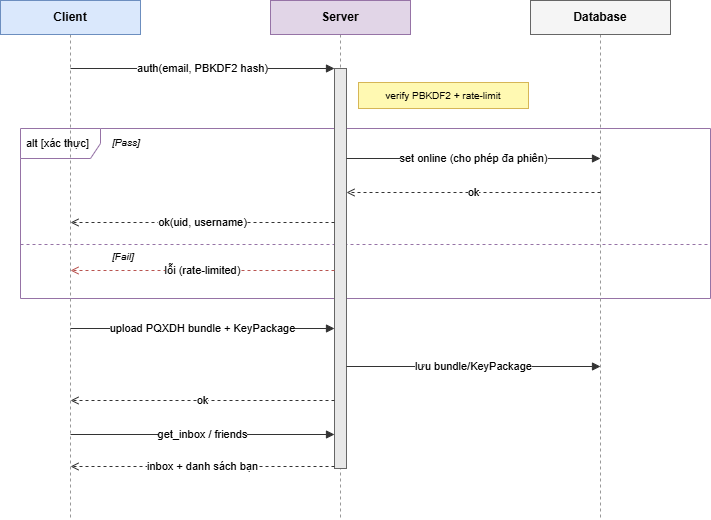
\includegraphics[width=0.85\linewidth]{Figure/SequenceLoginKeyPublish.png}
    \caption{Sơ đồ tuần tự: đăng nhập và công bố khóa}
    \label{fig:seq-login-key-publish}
\end{figure}

\textbf{Quy trình gửi tin nhắn DM E2EE}

Client lấy bundle của peer, kiểm tra proof identity với auditor, thực hiện bắt tay PQXDH để tạo root secret rồi gửi tin đã mã hóa; server chỉ lưu và chuyển tiếp ciphertext.

\begin{figure}[H]
    \centering
    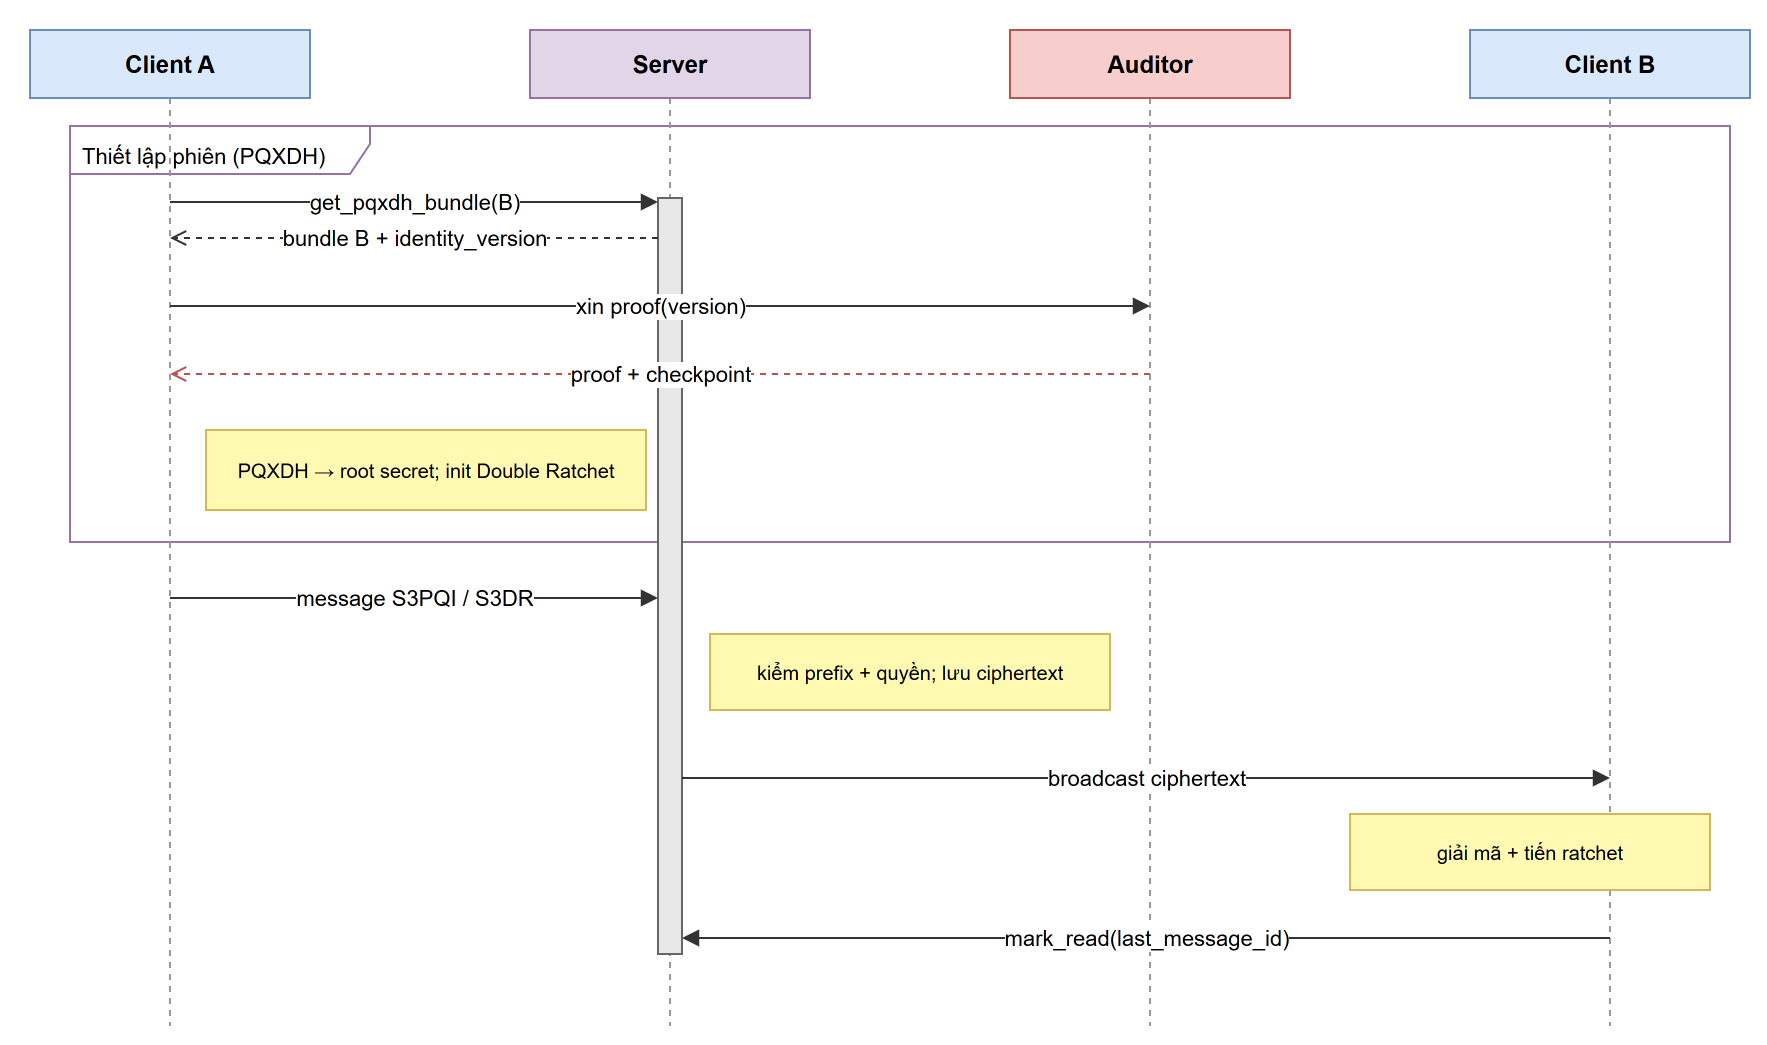
\includegraphics[width=0.9\linewidth]{Figure/SequenceDmE2ee.png}
    \caption{Sơ đồ tuần tự: gửi tin nhắn DM E2EE}
    \label{fig:seq-dm-e2ee}
\end{figure}

\textbf{Quy trình thay đổi thành viên group bằng MLS}

Mọi thay đổi membership đi qua hai bước \texttt{prepare} và \texttt{apply}; server chỉ áp dụng thay đổi sau khi MLS validator chấp nhận public state dựa trên \texttt{PublicGroup}.

\begin{figure}[H]
    \centering
    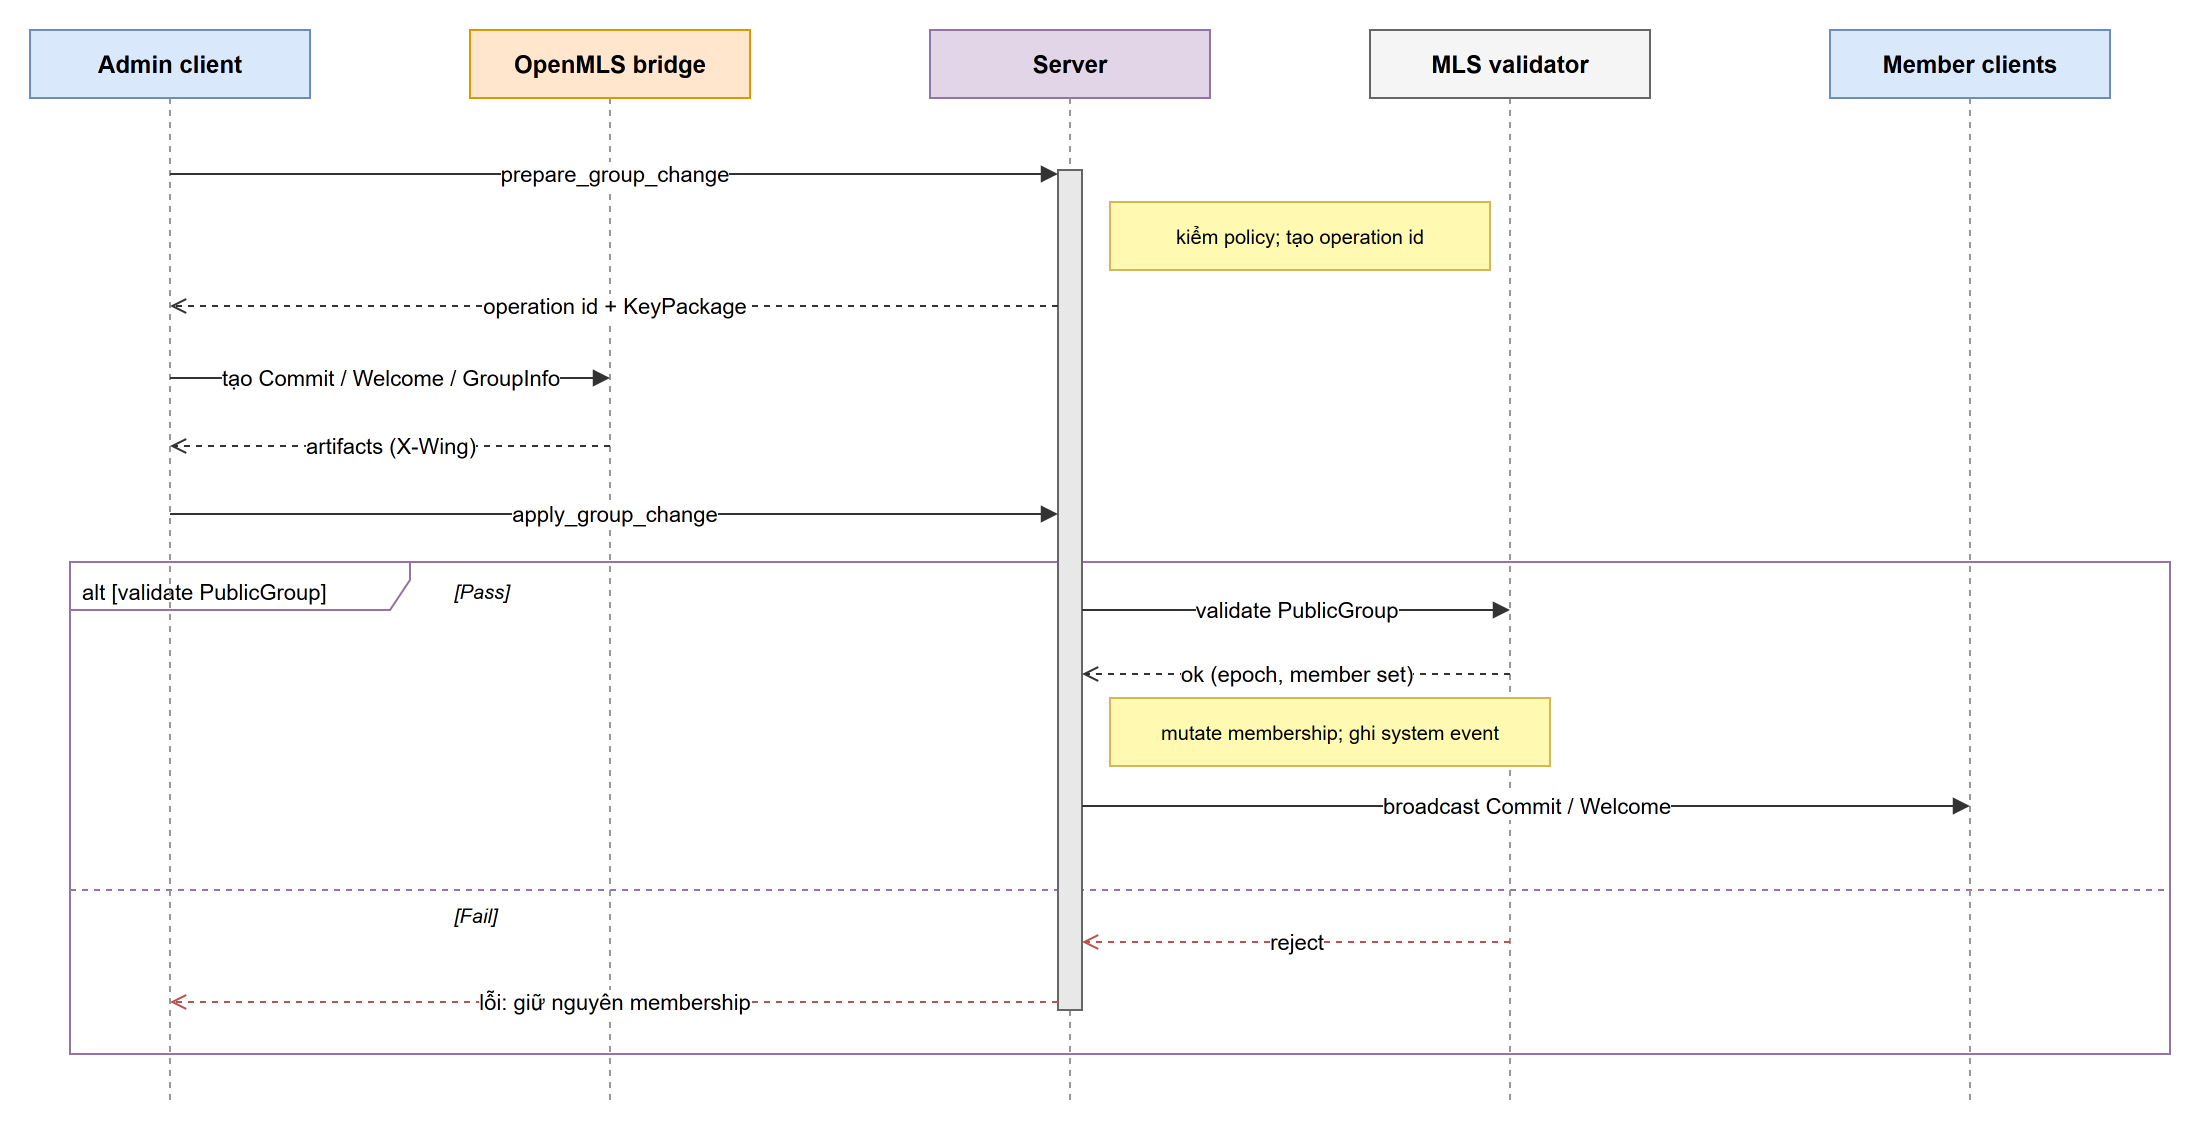
\includegraphics[width=0.95\linewidth]{Figure/SequenceGroupMlsValidation.png}
    \caption{Sơ đồ tuần tự: thay đổi thành viên group bằng MLS}
    \label{fig:seq-group-mls-validation}
\end{figure}

\textbf{Quy trình tải lịch sử, read cursor và system event}

Khi mở hội thoại, client cập nhật read cursor theo message id và tải lịch sử ciphertext cùng các system event để dựng lại timeline đúng thứ tự sau khi đăng nhập lại hoặc reload.

\begin{figure}[H]
    \centering
    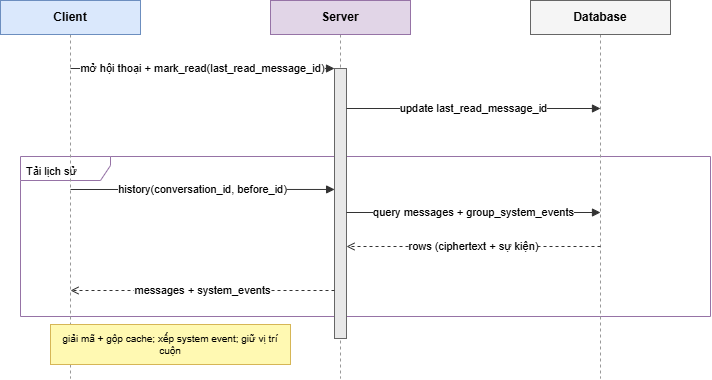
\includegraphics[width=0.85\linewidth]{Figure/SequenceHistoryReadSystemEvents.png}
    \caption{Sơ đồ tuần tự: tải lịch sử, read cursor và system event}
    \label{fig:seq-history-read-events}
\end{figure}

\section{Thiết kế giao thức bảo mật}\label{sec:security-protocol}

Yêu cầu thiết kế quan trọng nhất là server không được đọc nội dung tin nhắn người dùng. Tin nhắn phải được mã hóa ở client trước khi gửi lên server. Server có thể lưu, chuyển tiếp, sắp xếp và trả lịch sử, nhưng trường nội dung trong cơ sở dữ liệu phải là ciphertext có prefix hợp lệ của giao thức.

Với group, hệ thống dùng MLS theo RFC 9420 qua OpenMLS để quản lý epoch, secret tree, Welcome và Commit. Ciphersuite group là X-Wing hybrid, kết hợp ML-KEM-768 với X25519 cho confidentiality và dùng Ed25519 cho authentication; X-Wing hiện là bản nháp Internet-Draft (\texttt{draft-connolly-cfrg-xwing-kem}) mang tính thực nghiệm. Server phải từ chối KeyPackage không đúng ciphersuite, kiểm tra chữ ký SecChat trên KeyPackage, và validate public MLS state trước khi mutate membership.

Khóa bí mật của người dùng không được lưu thô. Client phải mã hóa identity key, prekey, ratchet state, group state và các file trạng thái E2EE bằng master key dẫn xuất từ mật khẩu. Khi người dùng đổi mật khẩu, các file nhạy cảm cục bộ phải được bọc lại bằng master key mới.

Client được tin tưởng để giữ plaintext, master key và trạng thái crypto. Server được tin tưởng để xác thực tài khoản, kiểm tra quyền trong group, validate public MLS state, lưu thứ tự tin nhắn và chuyển tiếp đúng người, nhưng không được tin tưởng để giữ bí mật nội dung tin.

Cơ sở dữ liệu được xem là có thể bị lộ. Vì vậy các secret quan trọng phải được lưu ở dạng mã hóa.


\subsection{Thiết kế mã hóa đầu cuối}

\subsubsection{Các lớp khóa}

SecChat tách khóa theo vai trò thay vì dùng một khóa chung cho toàn bộ hệ thống. Identity key Ed25519 gắn với danh tính bảo mật của tài khoản và dùng để ký prekey. Prekey X25519 và prekey ML-KEM dùng cho bắt tay DM kiểu PQXDH. Sau bắt tay, Double Ratchet state tạo message key riêng cho từng tin DM. Với group, OpenMLS giữ MLS group state, epoch secret và application secret; server chỉ thấy public state cần cho kiểm tra membership.

Cách chia này giúp mỗi khóa có vòng đời rõ ràng. Mật khẩu dùng để mở khóa local state, identity key dùng để nhận diện người dùng, prekey dùng để bắt tay phiên, còn message key dùng cho từng tin nhắn.

\begin{figure}[H]
    \centering
    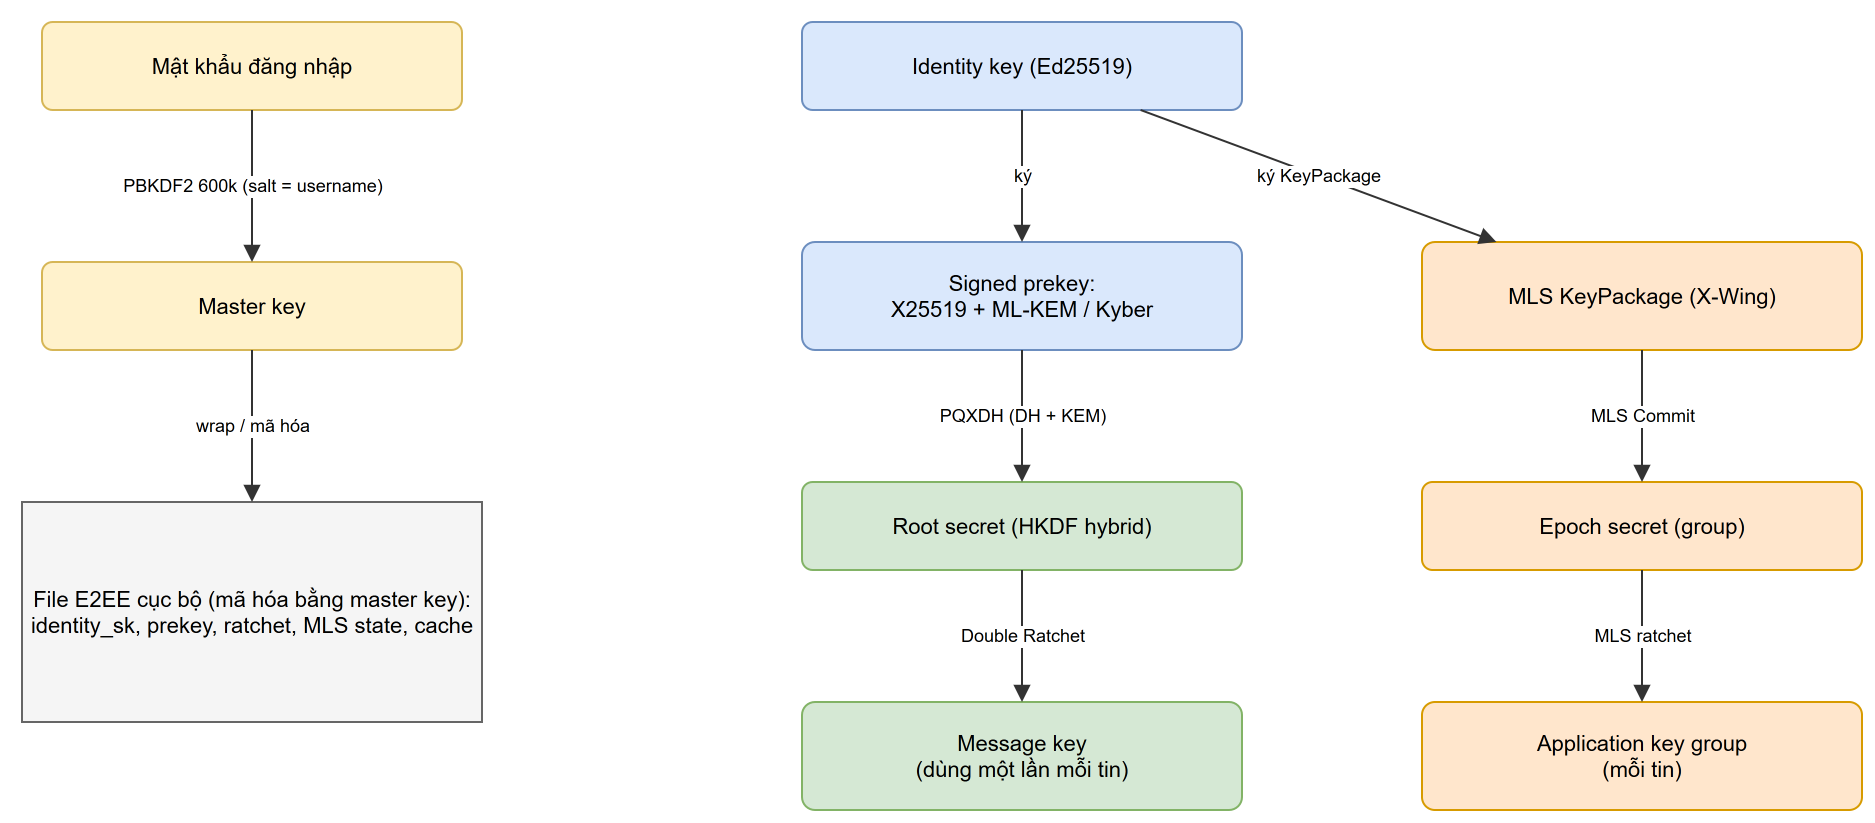
\includegraphics[width=0.9\linewidth]{Figure/KeyLifecycle.png}
    \caption{Vòng đời các khóa chính trong SecChat}
    \label{fig:keylifecycle}
\end{figure}

\subsubsection{Mật khẩu và master key}\label{subsubsec:password}

Ở tầng đăng nhập, client không gửi mật khẩu thô lên server. Client trước hết băm mật khẩu bằng PBKDF2-HMAC-SHA256 với salt là email đăng nhập. Server tiếp tục băm giá trị nhận được bằng PBKDF2 với salt ngẫu nhiên riêng trước khi lưu vào bảng \texttt{users}. Thiết kế này làm cho server không biết mật khẩu gốc.

Ở tầng bảo vệ file E2EE cục bộ, client dẫn xuất master key từ mật khẩu gốc và username thực tế do server trả về sau đăng nhập. Master key này dùng để mã hóa các file như identity secret key, prekey secret, ratchet state, group state, safety verification và plaintext cache. Khi đổi mật khẩu, client bọc lại các file này bằng master key mới để lịch sử và key cũ không bị mất.

\subsubsection{Prekey bundle kiểu PQXDH}

Mỗi client công bố một bundle khóa cho SecChat. Bundle gồm identity public key Ed25519, signed X25519 prekey, signed ML-KEM prekey, cùng các one-time prekey nếu còn. Bắt tay DM ưu tiên ML-KEM-1024 khi thư viện hỗ trợ, nhưng bundle vẫn ghi rõ thuật toán đang dùng để hai phía xử lý đúng. Server lưu bundle trong các bảng như \texttt{pqxdh\_bundles}, \texttt{pqxdh\_curve\_one\_time\_prekeys} và \texttt{pqxdh\_pq\_one\_time\_prekeys}.

Khi cùng một tài khoản đăng nhập trên thiết bị khác, nếu mở được identity secret, client sẽ tạo một PQXDH bundle mới cho thiết bị hiện tại và upload lại trước khi nhận hoặc gửi DM mới. Cách này giữ nguyên safety identity nhưng thay prekey theo máy đang active, tránh tình trạng server trả bundle có public prekey không khớp với secret cục bộ. Nếu server đang có bundle cũ nhưng client hiện tại thiếu private prekey, client vẫn phải publish bundle mới thay vì dựa vào trạng thái cũ.

Khi A muốn bắt đầu DM với B, A gọi \texttt{get\_pqxdh\_bundle}. Server trả bundle của B và chỉ cấp one-time prekey thuộc cùng generation với signed prekey hiện hành. Khi B publish bundle mới, server xóa batch one-time prekey cũ trước khi chèn batch mới; nhờ vậy người gửi không bị nhận signed prekey mới ghép với one-time prekey cũ. Bundle trả về có thêm \texttt{identity\_version}. Trước khi dùng bundle, client hỏi auditor service để lấy Merkle proof cho identity key và version đó. Kết quả audit được lưu vào security state của hội thoại: proof hợp lệ làm tăng độ tin cậy; proof, key, version hoặc checkpoint sai được ghi là \texttt{audit\_mismatch} với mã lỗi cụ thể; lỗi vận hành như auditor không truy cập được hoặc HTTP lỗi được ghi là \texttt{audit\_unavailable}. Client kiểm tra chữ ký prekey bằng identity key của B, sinh X25519 ephemeral, encapsulate vào ML-KEM public key của B, rồi trộn các DH secret và KEM secret bằng HKDF. Secret đầu ra dùng để khởi tạo Double Ratchet.

Identity transparency không thay thế safety number. Nó giúp client biết key đang dùng có nằm trong lịch sử identity đã được auditor ký hay không. Nếu safety number đổi, UI đánh dấu hội thoại là key changed và yêu cầu người dùng mở phần review để xem lịch sử identity trước khi tiếp tục gửi tin một cách bình thường. Nếu proof root không khớp, identity version không có trong log, identity key trong bundle khác log, checkpoint rollback, checkpoint split-view hoặc chữ ký checkpoint sai, UI hiển thị cảnh báo audit kèm nguyên nhân cụ thể. Nếu auditor tạm thời không truy cập được, UI cũng báo rõ đây là lỗi khả dụng của auditor, không đánh đồng với lỗi bằng chứng mật mã. Các cảnh báo này nhắc người dùng rằng chưa nên tin danh tính của đối phương nếu chưa so sánh safety number qua kênh ngoài SecChat. Cần phân biệt rõ hai loại: cảnh báo identity ở đây mang tính tư vấn, nghĩa là hệ thống hiển thị banner và trạng thái cần review nhưng không tự chặn cứng việc gửi tin, quyết định cuối cùng thuộc về người dùng; còn các lỗi crypto thật như chữ ký bundle sai, thiếu prekey cục bộ hoặc không có group Welcome thì làm việc mã hóa không thể tiếp tục.

\begin{figure}[H]
    \centering
    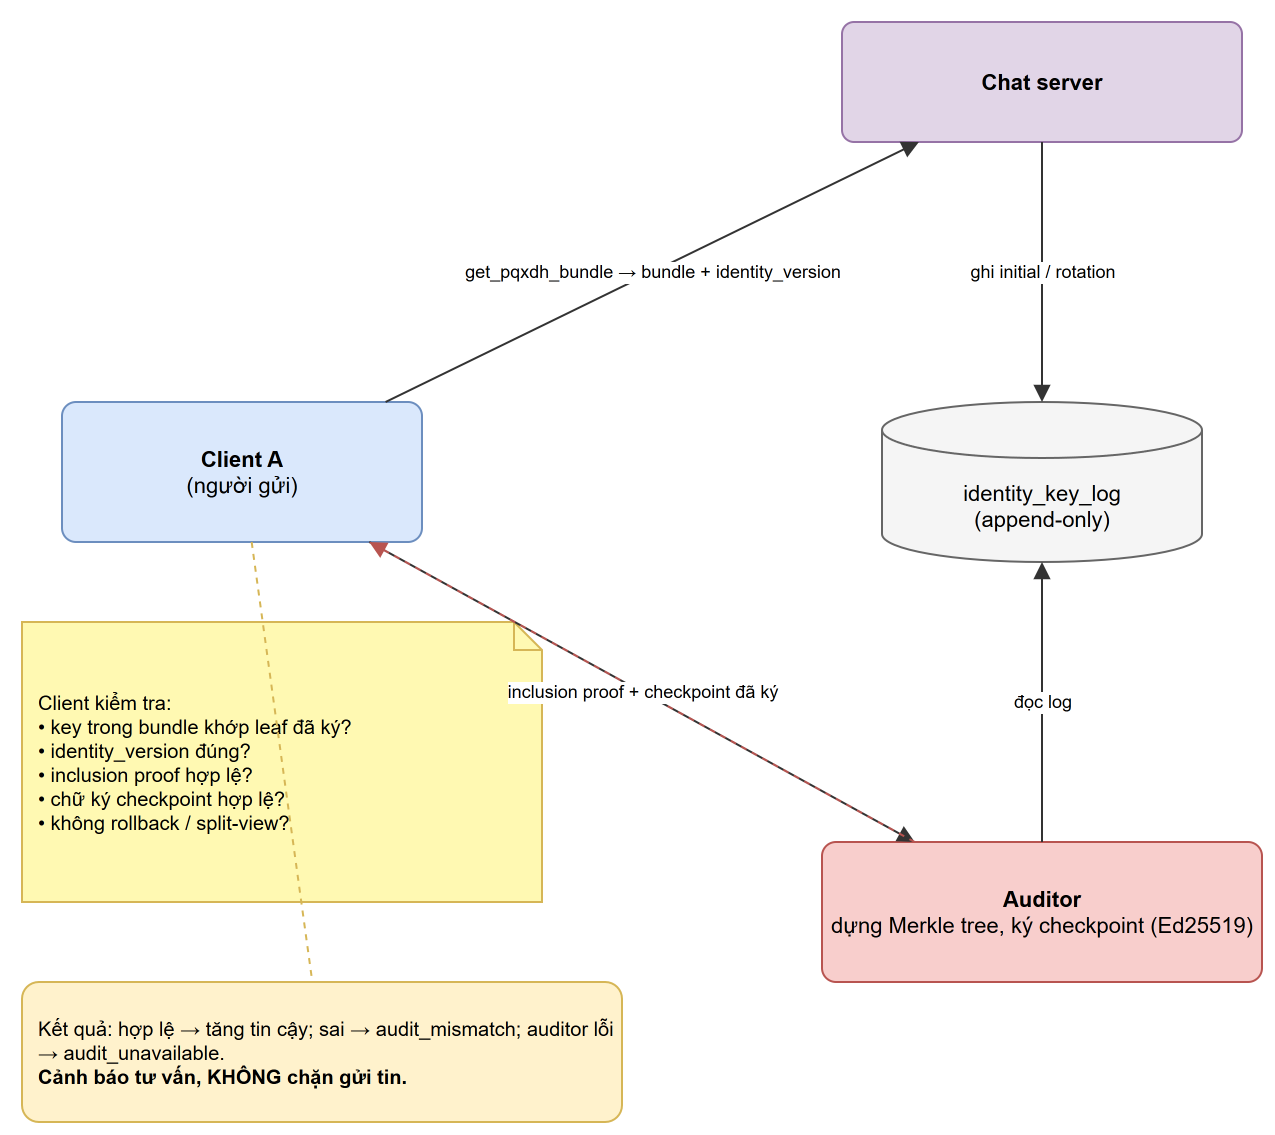
\includegraphics[width=0.9\linewidth]{Figure/IdentityTransparencyFlow.png}
    \caption{Luồng identity transparency giữa client, chat server và auditor}
    \label{fig:identitytransparencyflow}
\end{figure}

Tin nhắn đầu tiên của DM có prefix \texttt{S3PQI:}. Prefix này chứa transcript cần thiết để B tính lại cùng root secret và nhận tin đầu tiên. Sau đó các tin DM bình thường dùng prefix \texttt{S3DR:}. Toàn bộ trình tự lấy bundle, kiểm tra proof, sinh root secret rồi gửi tin đầu tiên được minh họa ở sơ đồ tuần tự~\ref{fig:seq-dm-e2ee}.

Chi tiết mật mã của bước bắt tay được trình bày ở Hình~\ref{fig:seq-pqxdh-kyber}: A trộn ba X25519 DH với shared secret ML-KEM-1024 bằng HKDF để tạo root secret; B decapsulate rồi tính lại đúng root đó. Đây là tính chất hybrid - kẻ tấn công phải phá đồng thời cả X25519 lẫn ML-KEM mới thu được root.

\begin{figure}[H]
    \centering
    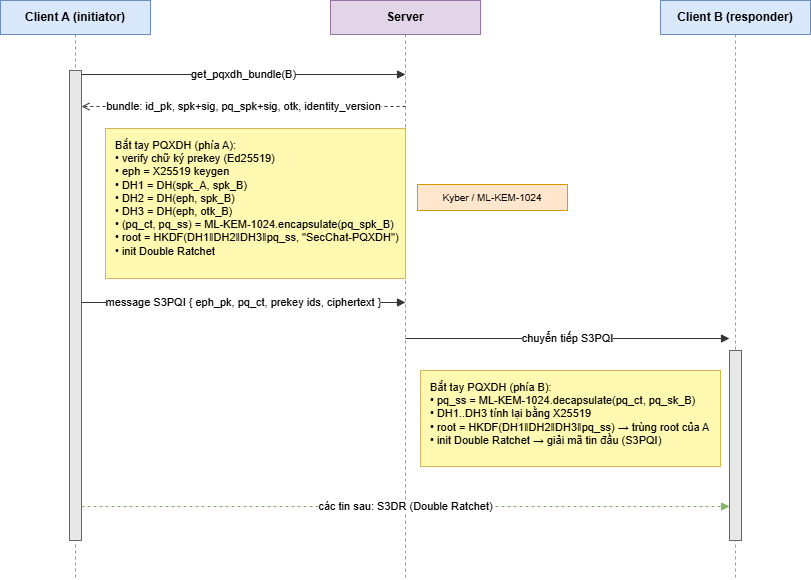
\includegraphics[width=0.92\linewidth]{Figure/SequencePqxdhKyber.png}
    \caption{Sơ đồ tuần tự: bắt tay PQXDH hybrid (X25519 + ML-KEM-1024)}
    \label{fig:seq-pqxdh-kyber}
\end{figure}

\subsubsection{Double Ratchet cho DM}

Sau khi DM được thiết lập, root key ban đầu lấy từ bắt tay PQXDH, rồi từ đó mỗi tin được mã hóa bằng một message key dùng một lần.

Về định dạng truyền, tin đầu tiên của phiên mang prefix \texttt{S3PQI} (gói kèm dữ liệu bắt tay PQXDH), các tin sau mang prefix \texttt{S3DR}. Bộ nhớ skipped-key được giới hạn 1000 khóa để chịu được tin offline và tin lệch thứ tự mà không bị làm cạn bộ nhớ. Toàn bộ trạng thái ratchet được mã hóa bằng master key rồi lưu trên đĩa, nên người dùng đăng xuất rồi đăng nhập lại vẫn tiếp tục đúng phiên mà không mất lịch sử.

\begin{figure}[H]
    \centering
    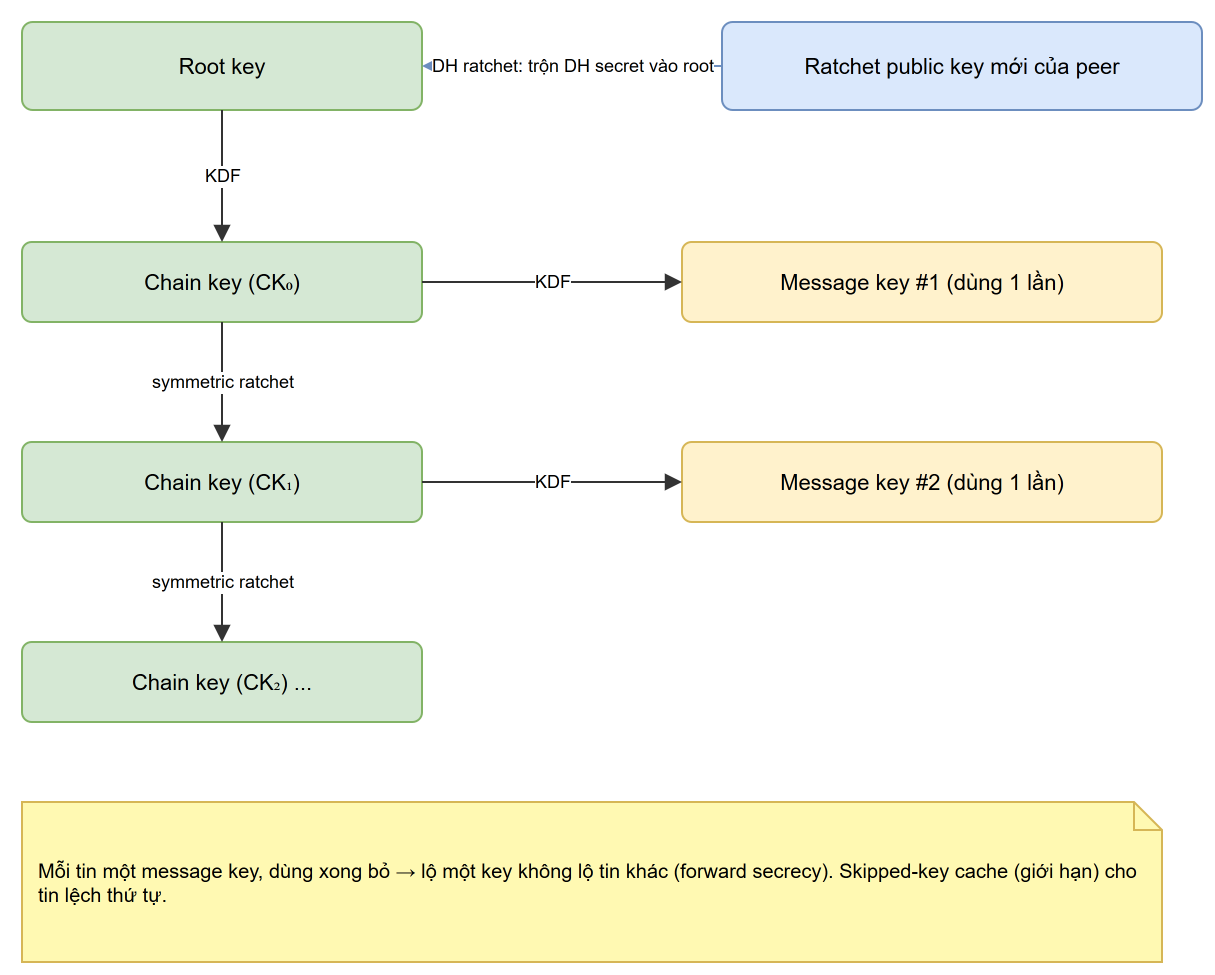
\includegraphics[width=0.9\linewidth]{Figure/DoubleRatchetFlow.png}
    \caption{Luồng Double Ratchet cho tin nhắn DM}
    \label{fig:doubleratchetflow}
\end{figure}


\subsubsection{Group MLS hậu lượng tử hybrid}\label{subsubsec:group-mls}

Nhóm chat không dùng Double Ratchet theo từng cặp mà dùng MLS với một group state chung có cấu trúc cây. SecChat hiện thực điều này bằng OpenMLS, chạy MLS theo RFC 9420 với ciphersuite X-Wing:
\begin{center}
    \small\texttt{MLS\_256\_XWING\_CHACHA20POLY1305\_SHA256\_Ed25519}
\end{center}
X-Wing là KEM hybrid kết hợp ML-KEM-768 và X25519, cung cấp bảo vệ hậu lượng tử cho confidentiality của group còn phần authentication của MLS sử dụng chữ ký Ed25519 cổ điển. Như đã nêu ở Chương 1, X-Wing hiện vẫn là một bản nháp Internet-Draft mang tính thực nghiệm chứ chưa phải chuẩn đã ổn định.

Mỗi thành viên công bố KeyPackage X-Wing sau khi đăng nhập. KeyPackage được ký thêm bằng SecChat identity key để server và client kiểm tra rằng package thuộc đúng tài khoản và đúng identity version. Server từ chối KeyPackage không đúng ciphersuite hoặc sai chữ ký trước khi lưu vào bảng \texttt{mls\_key\_packages}. Nếu client mở local MLS state cũ không còn khớp ciphersuite X-Wing, state đó bị bỏ và client công bố lại KeyPackage mới.

Mỗi thay đổi membership dùng Commit và GroupInfo do OpenMLS sinh. Luồng thay đổi bắt đầu bằng bước prepare: server kiểm tra policy như quyền admin, friend/block và KeyPackage còn chưa dùng. Client sau đó dùng OpenMLS bridge để tạo Commit, Welcome, GroupInfo và ratchet tree cần thiết, rồi gửi lại ở bước apply. Trước khi lưu handshake hoặc cập nhật bảng thành viên, server gọi validator OpenMLS dựa trên \texttt{PublicGroup}. Validator kiểm tra ciphersuite X-Wing, group id của conversation, epoch nối tiếp, credential của actor và member set sau commit có khớp operation đang chờ hay không. Trình tự prepare/apply giữa admin client, OpenMLS bridge, server và MLS validator được minh họa ở sơ đồ tuần tự~\ref{fig:seq-group-mls-validation}.

Public MLS state đã validate được lưu trong \texttt{mls\_group\_state}, gồm ciphersuite, public state base64, public state hash, backend validation và thời điểm validate. Server vẫn không giữ epoch secret, không sinh group secret và không giải mã MLS application bytes. Thành viên mới nhận Welcome dành riêng cho KeyPackage của mình và không mặc nhiên đọc được lịch sử trước khi tham gia. Thành viên bị xóa xử lý Commit remove thì group local inactive và không đọc được tin sau epoch mới.

Toàn bộ vòng đời khóa MLS - công bố KeyPackage X-Wing, tạo Commit/Welcome/GroupInfo, server validate \texttt{PublicGroup}, thành viên \texttt{join\_from\_welcome} và mã hóa application message (\texttt{S3MLS}) - được mô tả ở Hình~\ref{fig:seq-mls-group}.

\begin{figure}[H]
    \centering
    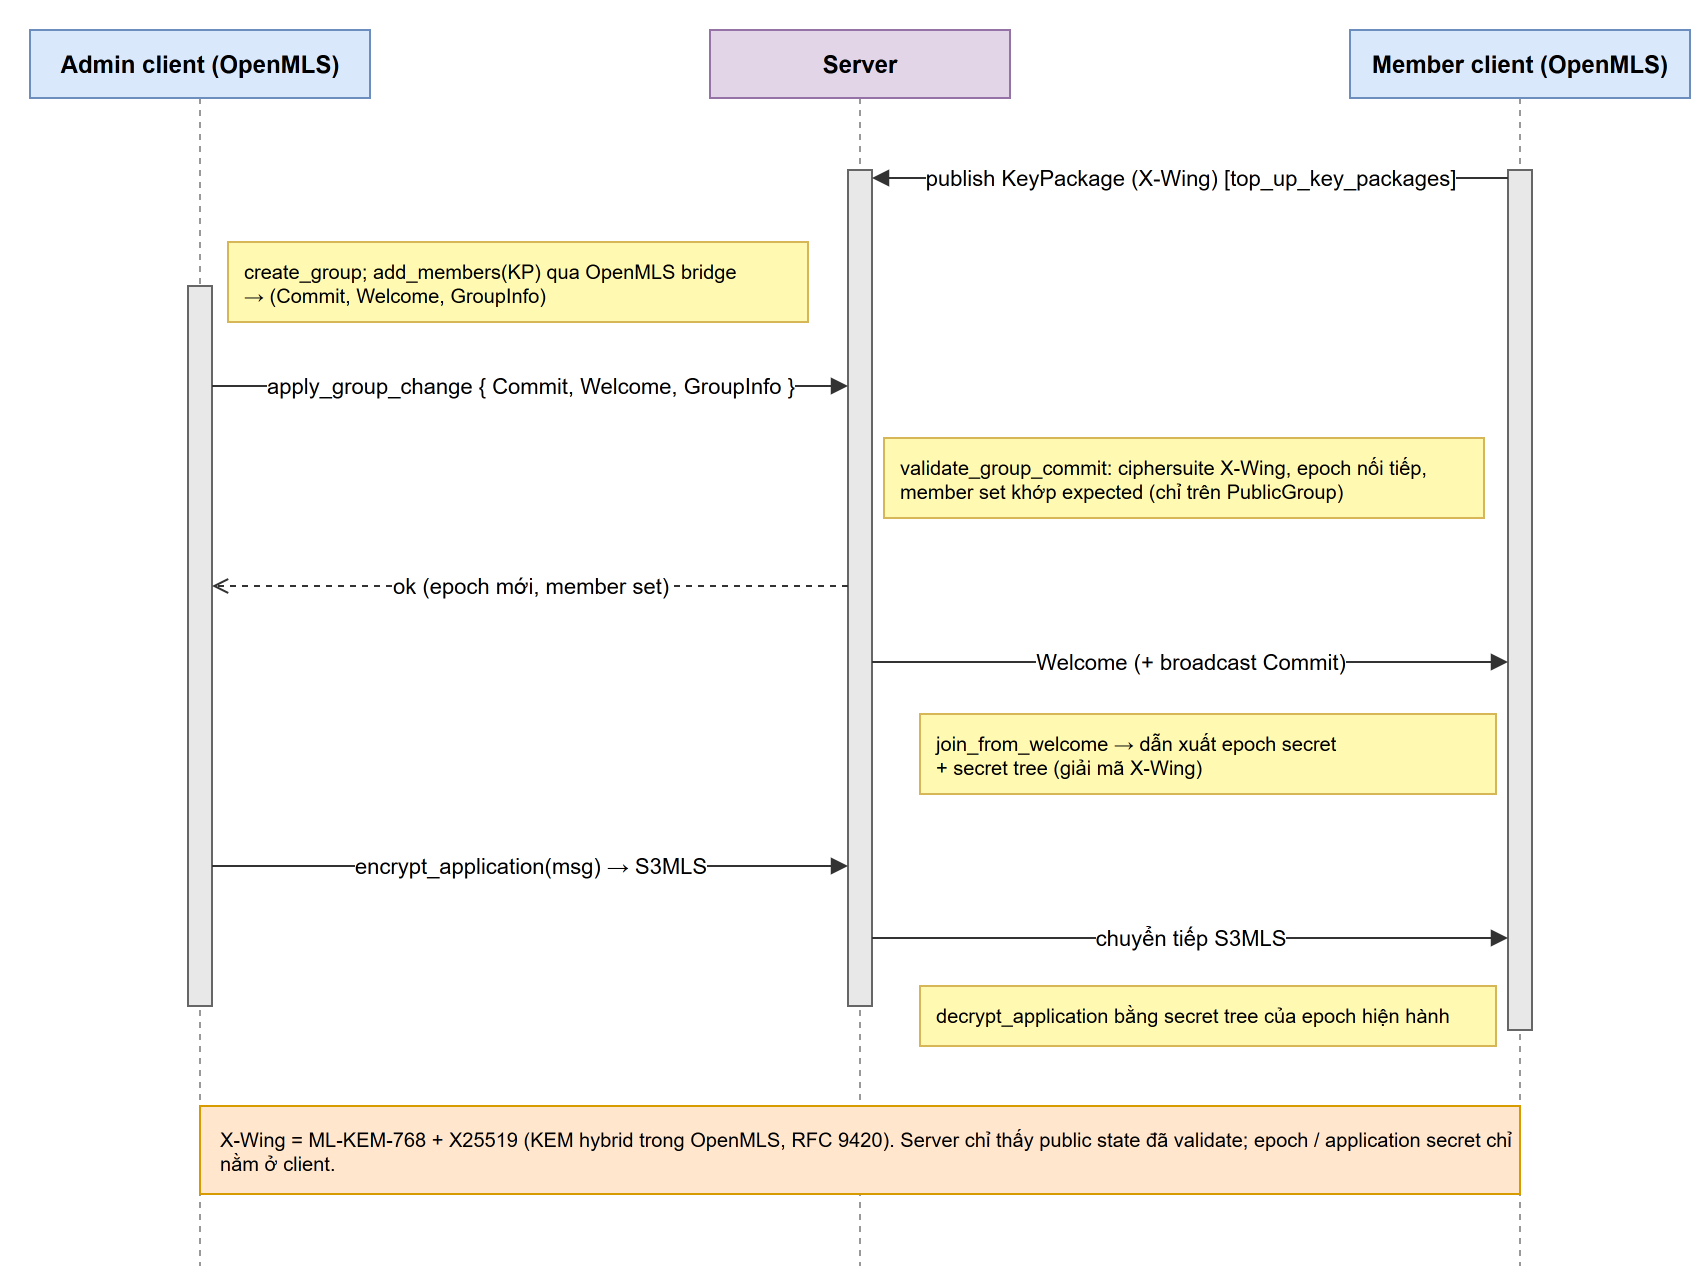
\includegraphics[width=0.92\linewidth]{Figure/SequenceMlsGroup.png}
    \caption{Sơ đồ tuần tự: vòng đời khóa group MLS X-Wing (KeyPackage $\rightarrow$ Commit/Welcome $\rightarrow$ epoch $\rightarrow$ application message)}
    \label{fig:seq-mls-group}
\end{figure}

Trạng thái verified trong DM không tự áp dụng cho group. Với group, client dựa vào MLS Welcome, Commit, GroupInfo, transcript checkpoint và kiểm tra identity từng thành viên để phát hiện state không nối tiếp hoặc lịch sử bị sắp xếp bất thường.

\begin{figure}[H]
    \centering
    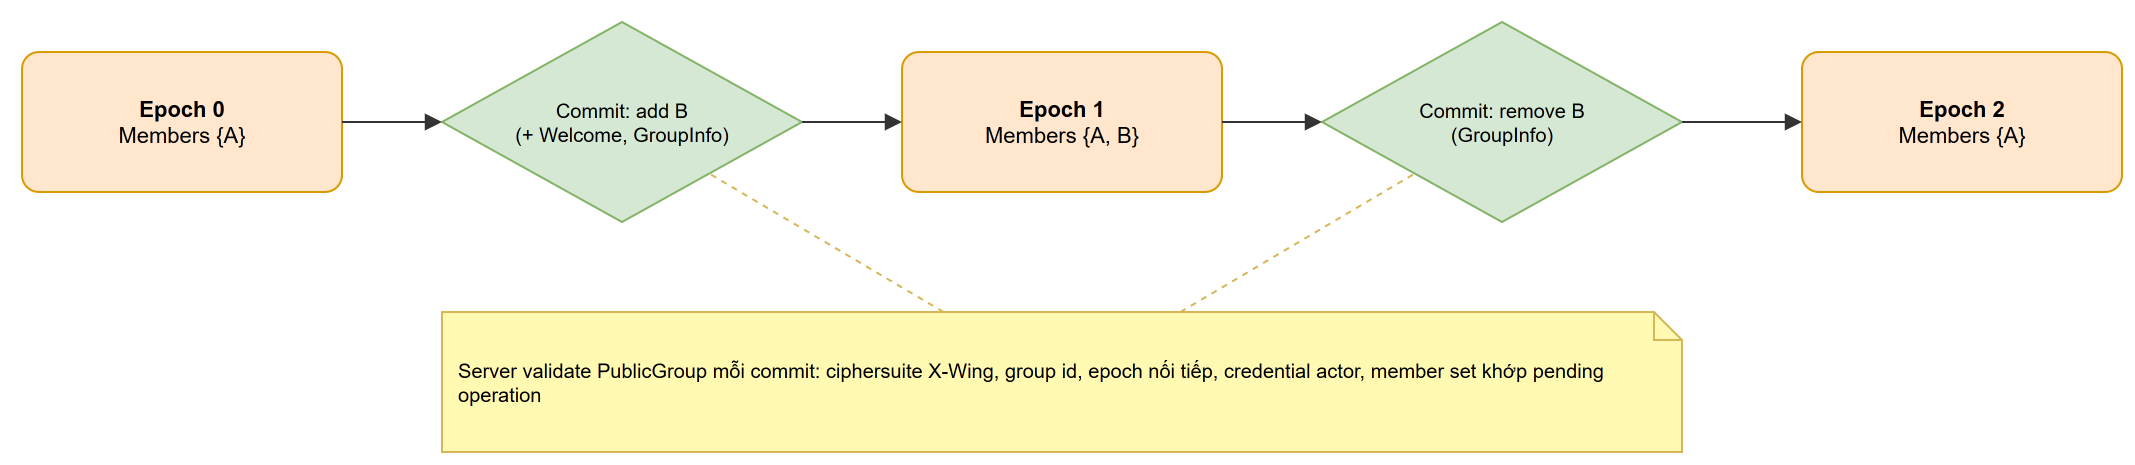
\includegraphics[width=0.9\linewidth]{Figure/GroupCommitChainFlow.png}
    \caption{Chuỗi MLS Commit dùng để kiểm tra thay đổi membership}
    \label{fig:groupcommitchainflow}
\end{figure}

Ngoài commit chain cho membership, client group còn có transcript checkpoint. Mỗi client tính hash nối tiếp trên các message đã chấp nhận, ký checkpoint bằng identity key và gửi checkpoint như một control message được mã hóa. Khi nhận checkpoint của thành viên khác, client so khớp với view cục bộ tại cùng message id. Nếu server bỏ sót message, đảo thứ tự hoặc cho hai client nhìn thấy history khác nhau, checkpoint có thể không khớp và UI sẽ có cơ sở để cảnh báo.

Khi có cảnh báo consistency, giao diện không chỉ ghi một dòng thông báo chung. Header hội thoại hiển thị trạng thái cảnh báo history và có nút Details để người dùng xem nội dung cụ thể của cảnh báo, ví dụ commit chain không nối tiếp, thiếu sự kiện membership hoặc transcript checkpoint không khớp. Cơ chế này không làm server mất khả năng gây từ chối dịch vụ, nhưng giúp client phát hiện và trình bày rõ hơn các trường hợp server trả view không nhất quán.

\begin{figure}[H]
    \centering
    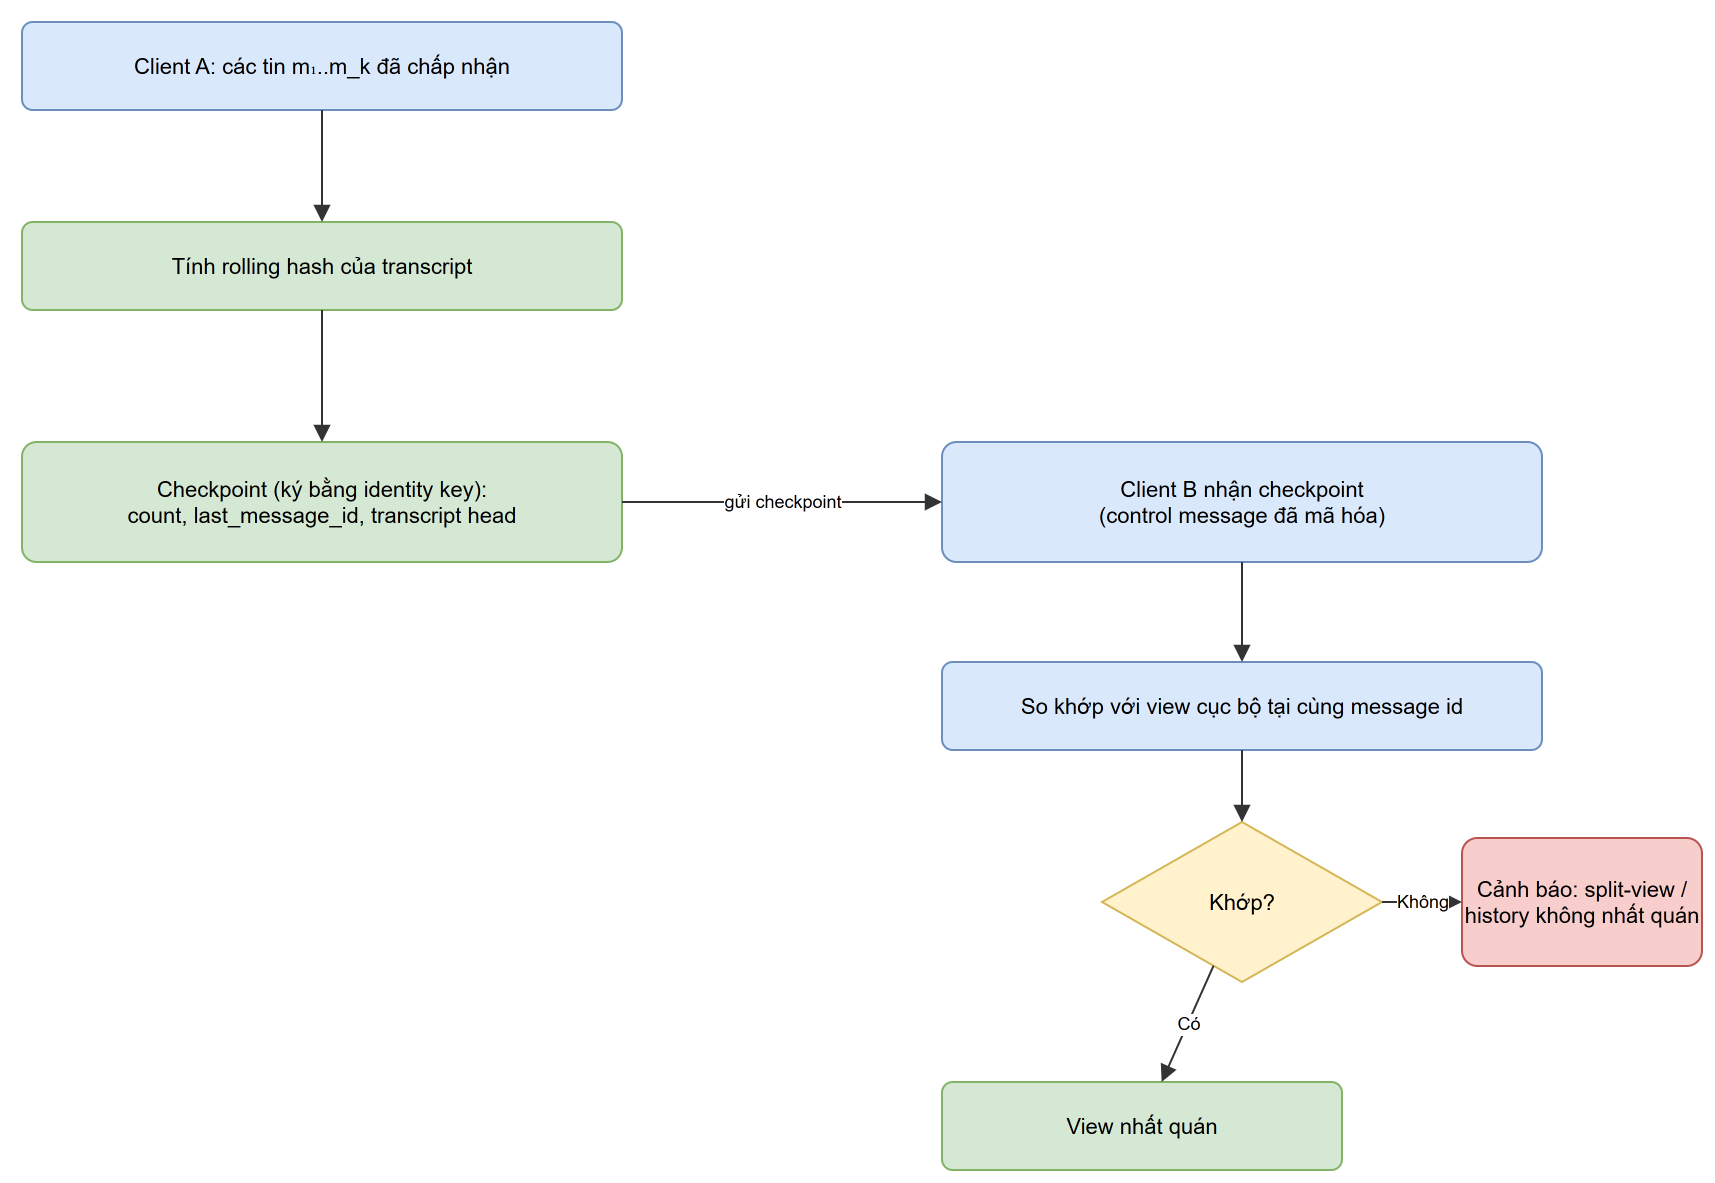
\includegraphics[width=0.9\linewidth]{Figure/TranscriptConsistencyFlow.png}
    \caption{Transcript checkpoint giúp phát hiện group history không nhất quán}
    \label{fig:transcriptconsistencyflow}
\end{figure}

\subsubsection{Local plaintext cache}

Vì Double Ratchet có tính forward secrecy, không phải mọi tin cũ đều có thể được giải mã lại vô hạn chỉ từ state hiện tại. Để trải nghiệm người dùng không bị mất lịch sử sau khi đăng xuất rồi đăng nhập lại, client lưu một cache plaintext cục bộ đã mã hóa bằng master key.

Đây là một đánh đổi có chủ ý. Cache giúp người dùng đọc lại lịch sử và giúp inbox preview hiển thị nội dung thật. Đổi lại, nếu attacker lấy được máy người dùng và mở được local state, lịch sử đã cache có thể bị đọc. Vì vậy UI có thiết lập bật hoặc tắt cache, thời gian giữ cache, xóa cache thủ công, xóa cache khi logout và tắt cache cho từng conversation nhạy cảm. Backup E2EE cũng phải cho người dùng chọn có đưa cache vào file backup hay không.

Cache được tách theo tài khoản và theo thư mục chạy của client, nên việc đổi sang tài khoản khác trên cùng thiết bị không được xóa cache của tài khoản cũ. Khi tài khoản cũ đăng nhập lại đúng thiết bị đó, các tin đã từng decrypt phải được lấy lại từ cache và hiển thị đúng thứ tự. Nếu một tài khoản mới được thêm vào group sau này, hoặc cùng tài khoản đăng nhập ở thiết bị khác chưa có cache, các ciphertext cũ không giải mã được sẽ bị ẩn khỏi UI thay vì hiện placeholder lỗi giải mã.

Backup E2EE là một snapshot do người dùng export và giữ bằng passphrase riêng, không phải cơ chế đồng bộ liên tục. Khi restore trên thiết bị mới, client giải mã snapshot, bọc lại bằng master key hiện tại, merge cache theo message id và công bố lại bundle mới dưới cùng identity nếu identity secret được khôi phục. Việc restore như vậy giúp khôi phục lịch sử đã có trong backup mà không làm thay đổi key của người đối thoại.

\begin{figure}[H]
    \centering
    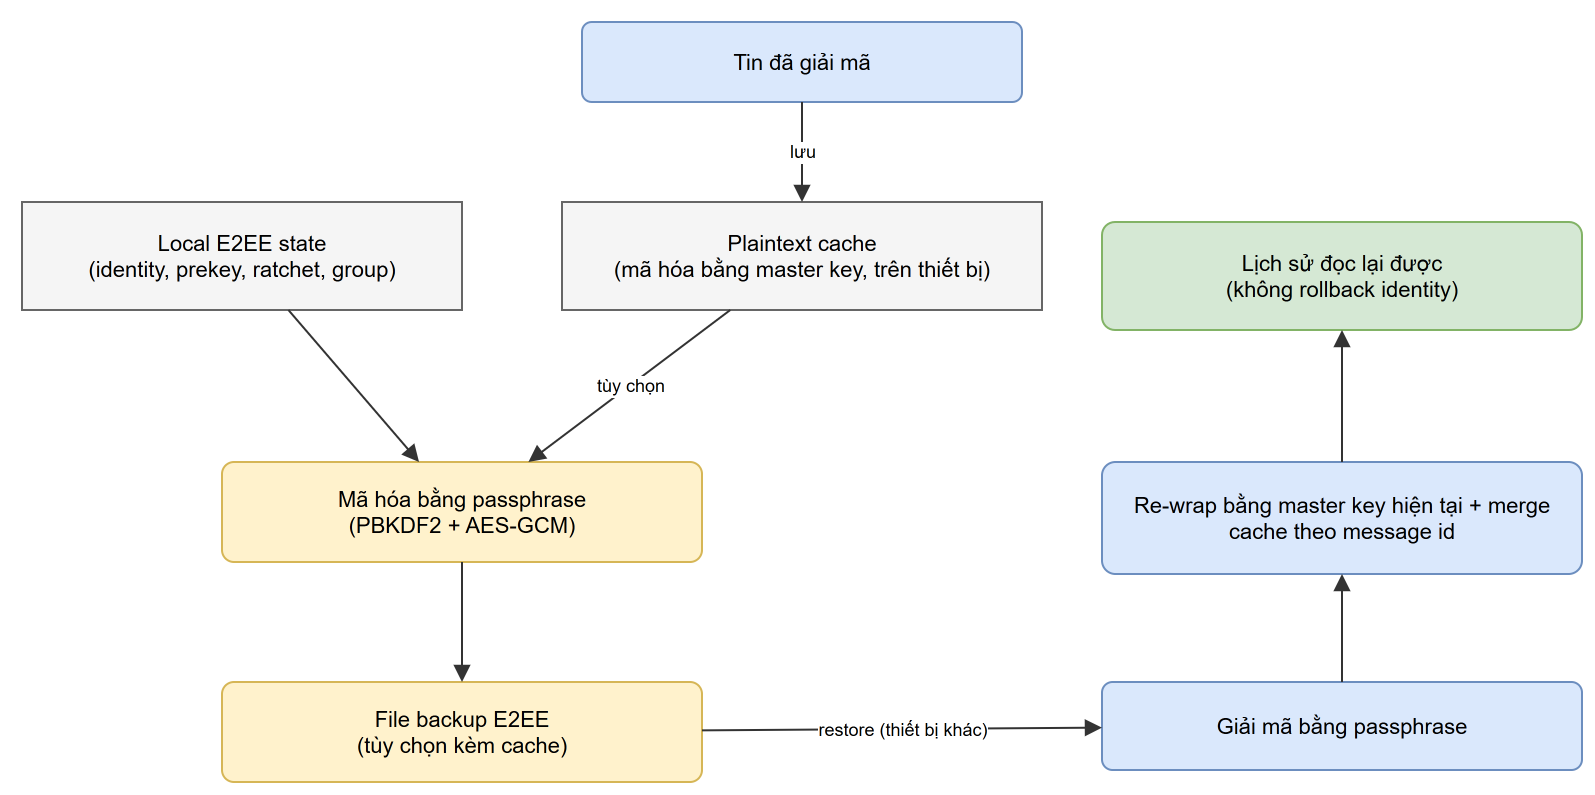
\includegraphics[width=0.9\linewidth]{Figure/CacheBackupFlow.png}
    \caption{Quan hệ giữa plaintext cache cục bộ và backup E2EE}
    \label{fig:cachebackupflow}
\end{figure}

\section{Thiết kế giao thức truyền tin}

\subsection{Các loại gói chính}

Các gói chính của giao thức được chia theo vai trò:
\begin{itemize}
    \item Nhóm xác thực gồm \texttt{register}, \texttt{auth} và \texttt{change\_password}.
    \item Nhóm hồ sơ gồm \texttt{get\_profile}, \texttt{update\_profile}, \texttt{upload\_avatar}, \texttt{remove\_avatar} và các lệnh privacy.
    \item Nhóm hội thoại gồm mở DM, tạo group, gửi message, tải history, lấy inbox và quản lý thành viên.
    \item Nhóm key gồm công bố identity, rotate identity, công bố PQXDH bundle, lấy PQXDH bundle và công bố MLS KeyPackage.
\end{itemize}

Các thay đổi membership dùng hai bước \texttt{prepare} và \texttt{apply}; chi tiết pending operation và validation public MLS state đã trình bày ở mục~\ref{subsubsec:group-mls}.

Nhóm message metadata xử lý pin, danh sách tin được ghim, reaction và typing indicator. Typing indicator có thể bị tắt vì đây là metadata nhạy cảm. Trạng thái unread chỉ áp dụng cho chính tài khoản hiện tại; hệ thống không gửi read receipt cho peer.

\subsection{Định dạng gói tin và quy trình đóng gói}\label{subsec:body-format}

Server chỉ chấp nhận message body có prefix E2EE hợp lệ. Với SecChat, các prefix chính là:

\begin{itemize}
    \item \texttt{S3PQI:} cho tin DM đầu tiên chứa transcript PQXDH-style.
    \item \texttt{S3DR:} cho tin DM sau khi đã vào Double Ratchet.
    \item \texttt{S3MLS:} cho tin group và encrypted group control message qua MLS.
\end{itemize}

Những prefix này là điều kiện bắt buộc để server lưu message mới. Nếu body không thuộc một trong ba dạng trên, server trả lỗi thay vì lưu dữ liệu, nhờ đó cơ sở dữ liệu không chứa plaintext message do client gửi nhầm.

\textbf{Quy trình đóng gói và mã hóa một tin DM.} Một tin nhắn trực tiếp được đóng gói ở client qua các bước sau trước khi rời thiết bị:
\begin{enumerate}
    \item Chuẩn bị plaintext. Nội dung văn bản được mã hóa UTF-8; nếu là tệp đính kèm thì client đặt một marker \texttt{FILE:} kèm dữ liệu tệp đã mã hóa base64 bên trong plaintext, nên với giao thức mọi tin đều là một khối plaintext thuần nhất.
    \item Lấy khóa và dựng header. Double Ratchet tiến chain key gửi để sinh một message key dùng một lần, đồng thời dựng header gồm khóa ratchet công khai hiện hành, số thứ tự tin và độ dài chain trước.
    \item Mã hóa có xác thực (AEAD). Plaintext được mã hóa bằng message key với header làm dữ liệu xác thực kèm theo (AAD), cho ra ciphertext và một thẻ xác thực; thẻ này ràng buộc cả header lẫn nội dung nên mọi sửa đổi đều bị phát hiện khi giải mã.
    \item Gắn prefix và đóng khung. Header, ciphertext và thẻ được nối lại, biểu diễn ở dạng văn bản base64 rồi gắn prefix \texttt{S3DR:} (riêng tin đầu phiên dùng \texttt{S3PQI:} và đính kèm transcript bắt tay PQXDH để phía nhận tái lập root secret).
    \item Bọc trong bản tin JSON và gửi qua TLS. Chuỗi có prefix được đặt vào trường \texttt{body} của một bản tin JSON; các trường định tuyến như mã hội thoại, người gửi và thời điểm vẫn ở dạng rõ để server xử lý. Bản tin JSON được gửi trong một khung WebSocket nằm trong kênh TLS.
\end{enumerate}
Ở phía server, sau khi kiểm tra quyền và prefix hợp lệ, toàn bộ trường \texttt{body} (ciphertext) được lưu nguyên văn vào bảng \texttt{messages} và chuyển tiếp; server không hề giải mã. Phía nhận làm ngược lại: tách prefix, giải mã base64, tách header, tiến hoặc xoay ratchet để lấy đúng message key, rồi giải mã và kiểm tra thẻ AEAD trên cả header lẫn ciphertext; nếu thẻ không hợp lệ thì tin bị loại bỏ. Tin nhóm theo cùng nguyên tắc nhưng dùng lớp mã hóa application message của MLS (khóa lấy từ secret tree của epoch) và mang prefix \texttt{S3MLS:}.

Khác với một giao thức đường hầm có bố cục nhị phân cố định, gói tin SecChat là một envelope JSON được mã hóa base64 nên độ dài thay đổi theo nội dung; tuy vậy các thành phần mật mã bên trong đều có kích thước cố định. Với một tin DM (\texttt{S3DR}), các trường quan trọng và kích thước của chúng gồm:
\begin{itemize}
    \item Prefix \texttt{S3DR:} -- 5 byte ASCII, là điều kiện để server chấp nhận lưu.
    \item \texttt{sid} -- định danh phiên ngẫu nhiên 16 byte.
    \item \texttt{h} (header, đồng thời là AAD): khóa công khai ratchet X25519 \texttt{dh} 32 byte, hai bộ đếm \texttt{pn}/\texttt{n}, và các trường định tuyến \texttt{conversation\_id}, \texttt{sender\_uid}, \texttt{recipient\_uid}, \texttt{sender\_identity\_version}.
    \item \texttt{ct} -- kết quả AES-256-GCM gồm nonce 12 byte $\Vert$ ciphertext (dài bằng plaintext) $\Vert$ thẻ xác thực 16 byte; khóa là message key 32 byte do Double Ratchet sinh.
    \item \texttt{eh} -- một bản sao header được mã hóa thêm bằng header key để giấu metadata ratchet.
\end{itemize}
Riêng tin mở phiên (\texttt{S3PQI}) mang thêm transcript bắt tay PQXDH: khóa định danh Ed25519 32 byte, signed prekey X25519 32 byte kèm chữ ký Ed25519 64 byte, một khóa ephemeral X25519 32 byte và ciphertext ML-KEM-1024 dài 1568 byte. Toàn bộ cấu trúc gói tin cùng hành trình mã hóa -- truyền -- giải mã được tổng hợp ở Hình~\ref{fig:packet-format}.

\begin{figure}[H]
    \centering
    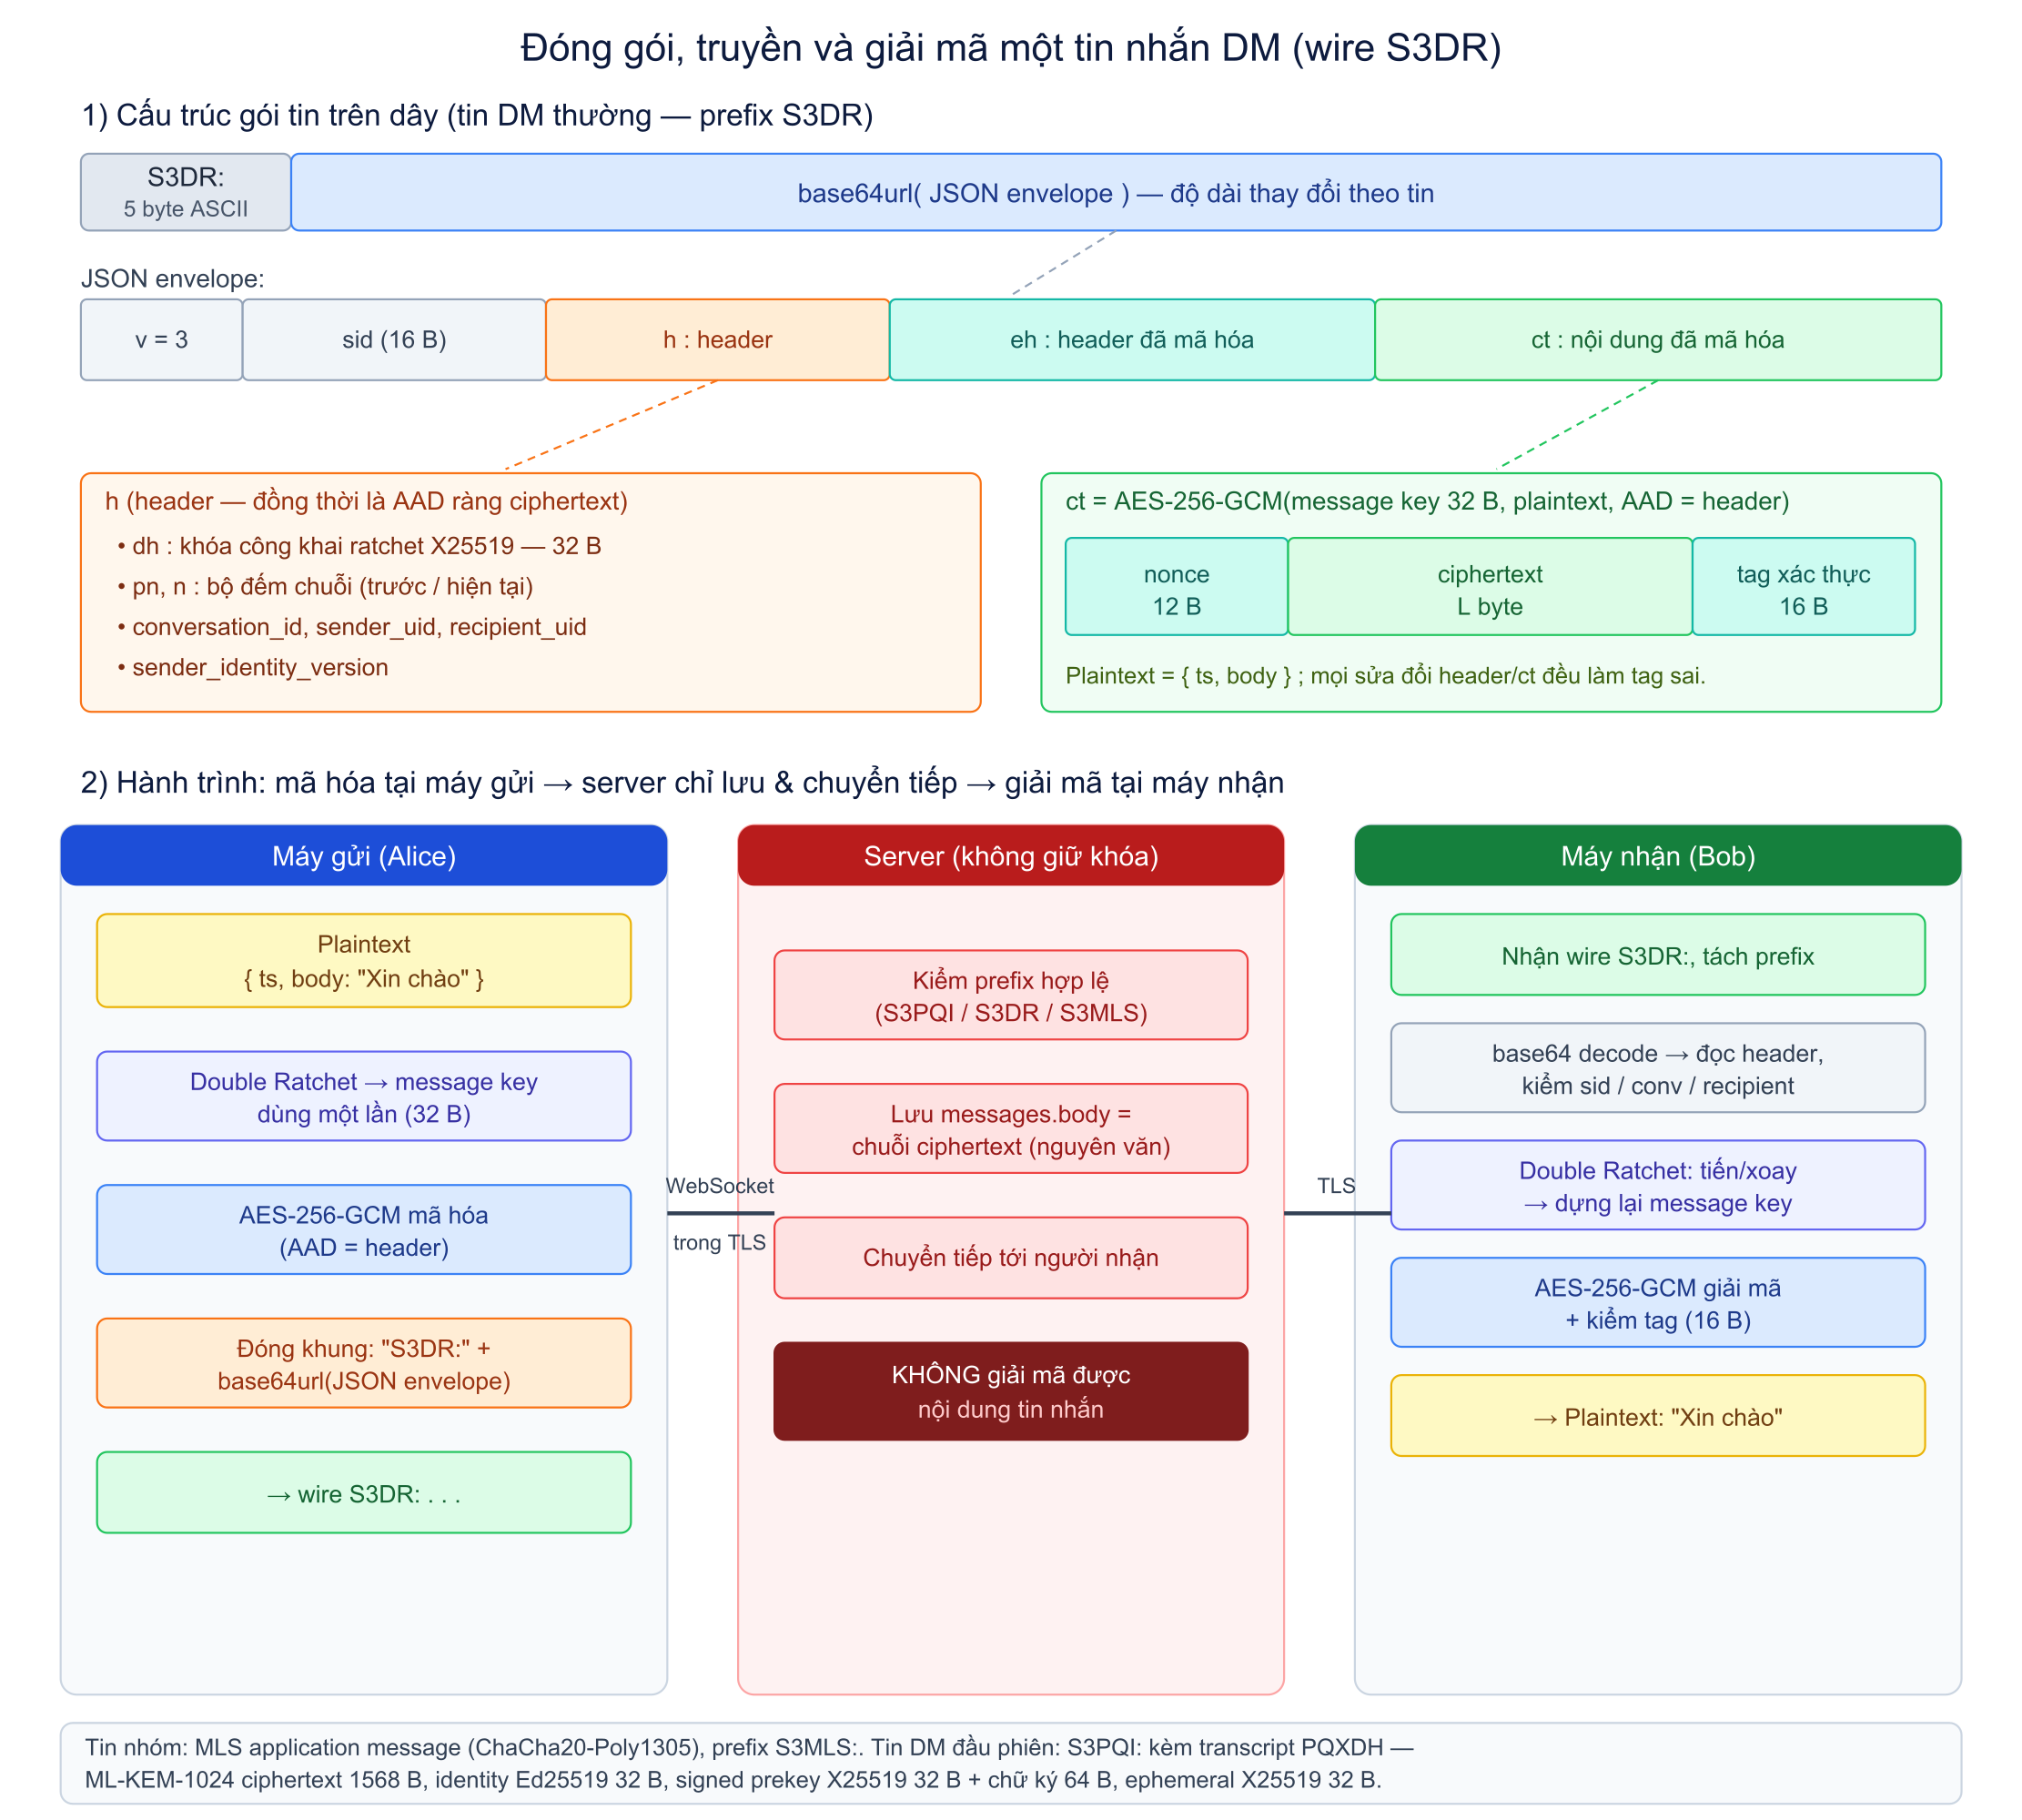
\includegraphics[width=\linewidth]{Figure/MessagePacketFormat.png}
    \caption{Cấu trúc gói tin S3DR và hành trình đóng gói, truyền, giải mã một tin DM}
    \label{fig:packet-format}
\end{figure}

\begin{figure}[H]
    \centering
    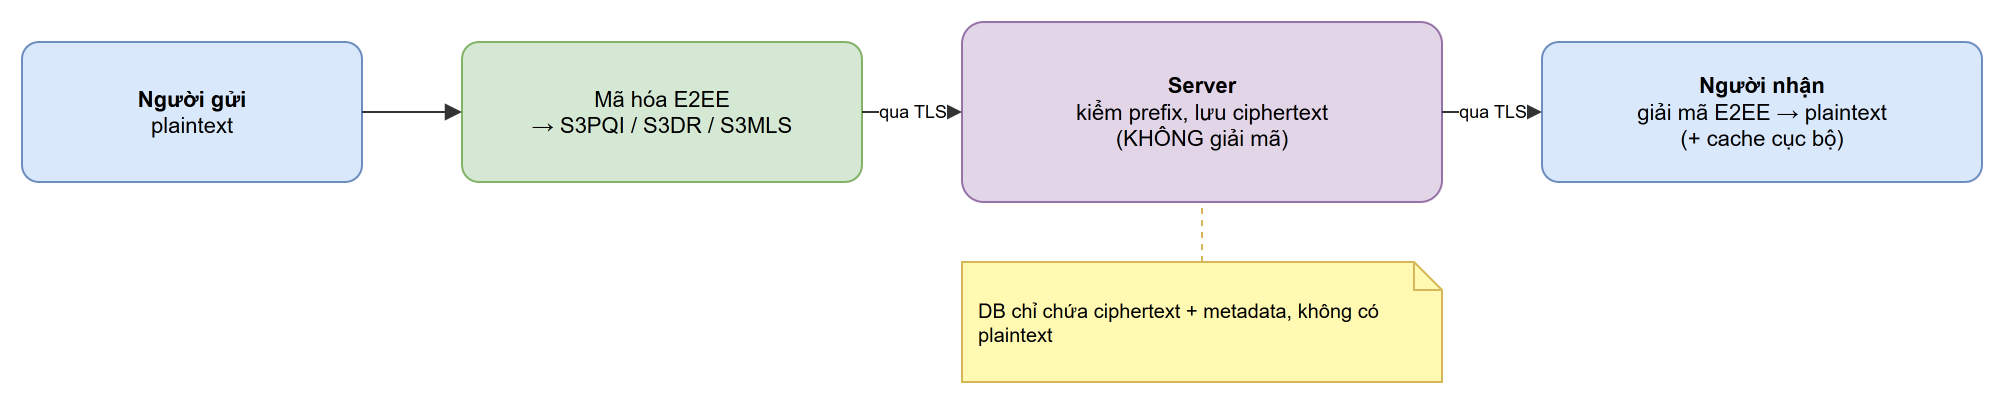
\includegraphics[width=0.9\linewidth]{Figure/MessageDataFlow.png}
    \caption{Data flow của một tin nhắn đã mã hóa đầu cuối}
    \label{fig:messagedataflow}
\end{figure}

\subsection{Metadata và quyền riêng tư}

Theo mô hình tin cậy ở mục~\ref{sec:security-protocol}, hệ thống chỉ bảo vệ nội dung tin nhắn, còn metadata vẫn nằm trong phạm vi tin cậy của server. Server cần metadata để vận hành inbox, group membership, history, pin, reaction và trạng thái unread cục bộ. Đây là giới hạn quan trọng của thiết kế và được đánh giá kỹ hơn ở chương thực nghiệm.

\section{Thiết kế client}

\subsection{Tổ chức mã nguồn}

Client được chia thành các phần chính. \texttt{client/pages} chứa các trang giao diện như đăng nhập, đăng ký và chat. \texttt{client/network.py} quản lý kết nối WebSocket qua TLS. \texttt{client/dialogs.py} chứa các dialog hồ sơ, avatar, đổi mật khẩu và thiết lập phụ. \texttt{client/crypto\_engine} chứa phần giao thức và trạng thái crypto.

Package \texttt{client/crypto\_engine} chứa primitive của giao thức như tạo bundle, kiểm tra chữ ký prekey, transcript kiểu PQXDH, Double Ratchet và wrapper OpenMLS. \texttt{client/crypto\_engine/openmls\_bridge.py} gọi bridge Rust dùng ciphersuite X-Wing. \texttt{client/crypto\_engine/session.py} quản lý state của phiên người dùng, file key mã hóa, cache plaintext mã hóa, trạng thái ratchet, trạng thái MLS group và mã hóa tin gửi đi.

\begin{figure}[H]
    \centering
    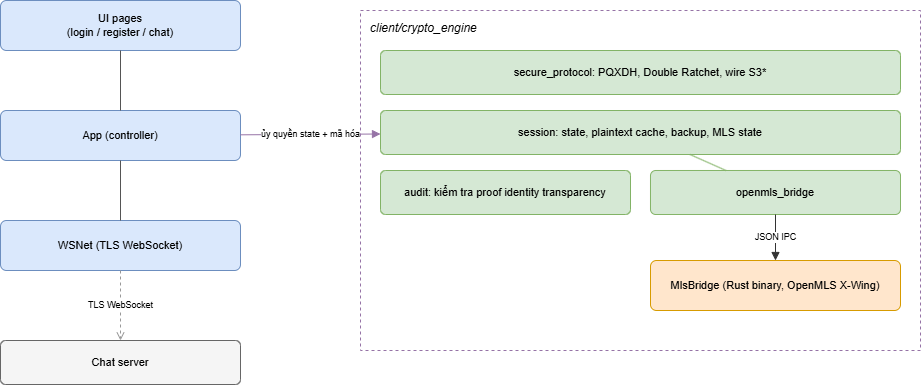
\includegraphics[width=0.9\linewidth]{Figure/CryptoEngineSplit.png}
    \caption{Ranh giới giữa UI controller và crypto engine}
    \label{fig:cryptoenginesplit}
\end{figure}

\subsection{Vai trò của App}

\texttt{client/app.py} là controller chính của ứng dụng PyQt. Nó nhận tín hiệu từ UI, gửi lệnh qua WebSocket, nhận event từ server và cập nhật giao diện. Controller này không sở hữu trực tiếp toàn bộ crypto state; các thao tác như lưu identity key, lưu prekey, lưu ratchet state, lưu group state, cache message, rotate identity và encrypt outbound message được ủy quyền cho \texttt{CryptoSession}.

Một phần decrypt message nhận vào và replay history vẫn được \texttt{App} điều phối cùng \texttt{CryptoSession}. Cách tổ chức này giữ UI controller ở vai trò phối hợp sự kiện, còn state nhạy cảm vẫn thuộc crypto engine.

\subsection{Giao diện chat}

UI hỗ trợ các thao tác quen thuộc của ứng dụng chat: danh sách hội thoại, friend list, avatar, profile, đổi mật khẩu, privacy, block, typing indicator, reaction, pin và forward. Read receipt không nằm trong UI; trạng thái read/unread chỉ phục vụ quản lý inbox cục bộ. Các hành động trên từng tin nhắn được gom vào nút ba chấm để tránh làm rối vùng timestamp. Forward hiển thị nhãn nhỏ, edit hiển thị trạng thái đã sửa, reaction hiển thị chip dưới tin nhắn, còn tin được ghim có badge và xuất hiện trong danh sách Pins.

Message view dùng \texttt{MessageListView} dựa trên \texttt{QScrollArea}, trong đó mỗi message là một row widget có layout riêng. Cách này phù hợp với các thao tác như menu ba chấm, reaction chip, badge pin, drag-drop file và trạng thái gửi.

\section{Thiết kế server}

\subsection{Kiến trúc phân tầng}

Server C được tách thành các lớp rõ ràng. \texttt{transport} xử lý socket, WebSocket, danh sách client và HTTP control plane. \texttt{protocol} xử lý JSON. \texttt{infra} chứa cấu hình, log, crypto helper, metrics, database pool, migration và rate limit. \texttt{domain} chứa validation. \texttt{repository} chứa truy vấn SQL. \texttt{services} chứa logic nghiệp vụ: auth, messaging, groups, keys, friends, profile, presence, blocking, notifications, reaction, pin, disappearing và conversation preferences (cùng dispatcher \texttt{chat}).

Việc tách lớp giúp \texttt{main.c} không phình thành một file chứa mọi nghiệp vụ. Khi có lệnh mới, service tương ứng xử lý qua dispatcher riêng, còn repository chịu trách nhiệm truy cập database bằng prepared statement.

\subsection{Xác thực, rate limit và đổi mật khẩu}

Cơ chế băm mật khẩu hai tầng client–server và dẫn xuất master key đã trình bày ở mục~\ref{subsubsec:password}. Ở góc độ server, điểm cần nhấn mạnh là server chỉ thao tác trên hash nhận từ client nên không bao giờ thấy mật khẩu gốc; khi đổi mật khẩu, server kiểm tra hash cũ rồi lưu hash mới, còn việc bọc lại local E2EE state bằng master key mới do client tự thực hiện. Nếu mật khẩu sai, server trả lỗi để UI báo rõ là email hoặc mật khẩu không đúng.

Rate limit được áp dụng cho luồng xác thực để giảm rủi ro brute-force. Log không nên ghi trực tiếp email hoặc dữ liệu nhạy cảm.

\subsection{Lưu và chuyển tiếp message}

Khi nhận message, server kiểm tra người gửi có quyền trong conversation và body có prefix E2EE hợp lệ (mục~\ref{subsec:body-format}), nhưng không giải mã message. Sau khi lưu vào bảng \texttt{messages}, server phát event cho các thành viên đang online; nếu người nhận offline, message vẫn nằm trong lịch sử và inbox giúp client tải lại khi người đó đăng nhập. Riêng edit message được lưu theo hướng event-sourced - thêm một row event trỏ về tin gốc qua \texttt{edit\_target\_message\_id} thay vì ghi đè ciphertext cũ - nhờ đó bản gốc không bị mất.

\subsection{Group và MLS validation}

Quy trình hai bước \texttt{prepare}/\texttt{apply} cùng các kiểm tra của MLS validator trên \texttt{PublicGroup} đã được mô tả ở mục~\ref{subsubsec:group-mls}. Ở góc độ server, điểm cần nhấn mạnh là server không bao giờ chỉ nhận base64 artifact rồi cập nhật thẳng bảng thành viên: mọi thay đổi membership chỉ được ghi sau khi validation pass, ngược lại handshake không được lưu và membership giữ nguyên. Vì chỉ làm việc trên public state, server có đủ dữ liệu để từ chối Commit giả mạo hoặc nằm ngoài policy nhưng không có application secret để đọc nội dung group. Các artifact MLS đã validate được lưu để thành viên replay Welcome/Commit đúng thứ tự khi online lại hoặc tải lại history.

\subsection{Vận hành và giám sát}

Server có HTTP control plane để trả health, readiness và metrics. Server GUI dùng dữ liệu này để hiển thị trạng thái vận hành qua các tab cần thiết như logs và metrics.


\newpage

\chapter{Cài đặt và đánh giá thực nghiệm}

\section{Môi trường cài đặt}

SecChat được triển khai trong môi trường Docker Compose để bảo đảm kết quả chạy có thể lặp lại. Môi trường sử dụng Windows 11, Docker Desktop, Python 3, PyQt5, C/OpenSSL cho server, MySQL 8.0 cho lưu trữ, Rust/OpenMLS cho MLS bridge và TigerVNC để quan sát nhiều client đồng thời. Cấu trúc triển khai gồm một container database, một container server, một container auditor và hai container client VNC.

\begin{figure}[H]
    \centering
    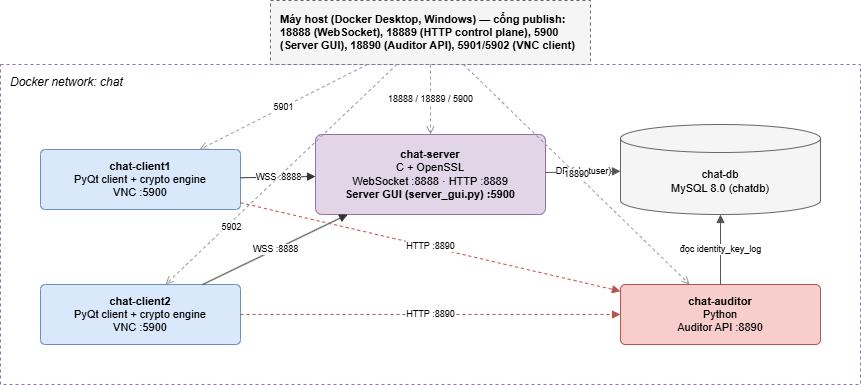
\includegraphics[width=0.95\linewidth]{Figure/DeploymentRuntime.png}
    \caption{Mô hình container khi chạy SecChat}
    \label{fig:deployment-runtime-ch3}
\end{figure}

Server WebSocket được expose tại cổng \texttt{18888}; HTTP control plane gồm \texttt{/healthz}, \texttt{/readyz} và \texttt{/metrics} được expose tại cổng \texttt{18889}. Hai client VNC dùng cổng \texttt{5901} và \texttt{5902}; server GUI dùng cổng \texttt{5900}. Trong môi trường thử nghiệm, các tài khoản \texttt{123@gmail.com}, \texttt{234@gmail.com} và \texttt{345@gmail.com} dùng mật khẩu \texttt{123456}. Các tài khoản và mật khẩu này chỉ phục vụ trình diễn cục bộ trong môi trường Docker, không được dùng trong triển khai thật. Trong môi trường thực tế, hệ thống cần bắt buộc chính sách mật khẩu mạnh và cấu hình các secret (mật khẩu cơ sở dữ liệu, khóa, chứng chỉ) riêng biệt thay vì các giá trị mặc định.

\section{Cài đặt và khởi động hệ thống}

Toàn bộ hệ thống có thể build và khởi động bằng Docker Compose. Lệnh sau tạo image, chạy migration và khởi động các service:

\begin{lstlisting}[language=bash]
docker compose up -d --build
\end{lstlisting}

Khi cần reset dữ liệu để kiểm tra lại từ trạng thái sạch, hệ thống được dừng kèm volume và khởi động lại:

\begin{lstlisting}[language=bash]
docker compose down -v
docker compose up -d --build
\end{lstlisting}

Endpoint \texttt{/readyz} được dùng để xác nhận server đã kết nối database và sẵn sàng nhận client. Khác với \texttt{/healthz}, readiness phản ánh trạng thái phụ thuộc vào MySQL nên phù hợp để kiểm tra trước khi chạy demo hoặc test.

\begin{figure}[H]
    \centering
    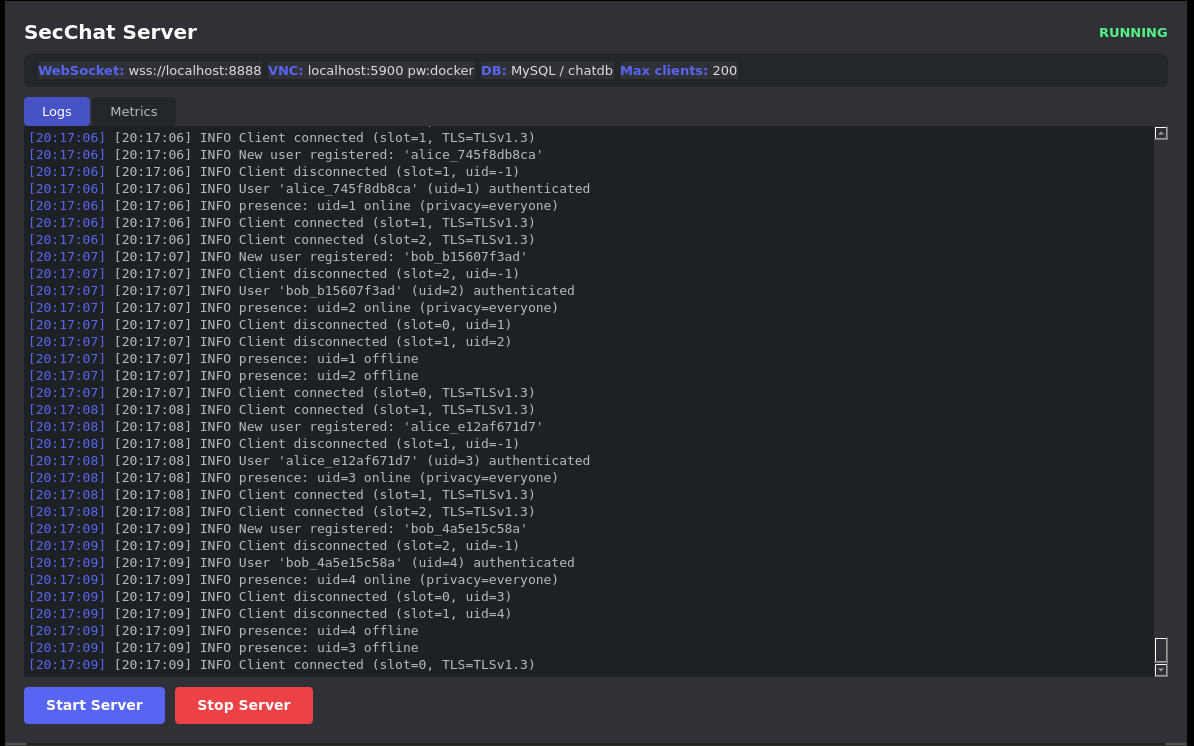
\includegraphics[width=0.95\linewidth]{Figure/ui_server_gui.png}
    \caption{Giao diện server khi hệ thống đang chạy}
    \label{fig:ui-server-gui-ch3}
\end{figure}

\section{Kết quả giao diện}

\subsection{Đăng nhập và danh sách hội thoại}

Sau khi đăng nhập, client mở local state E2EE, tải danh sách bạn bè, DM, group, request và các badge trạng thái.

\begin{figure}[H]
    \centering
    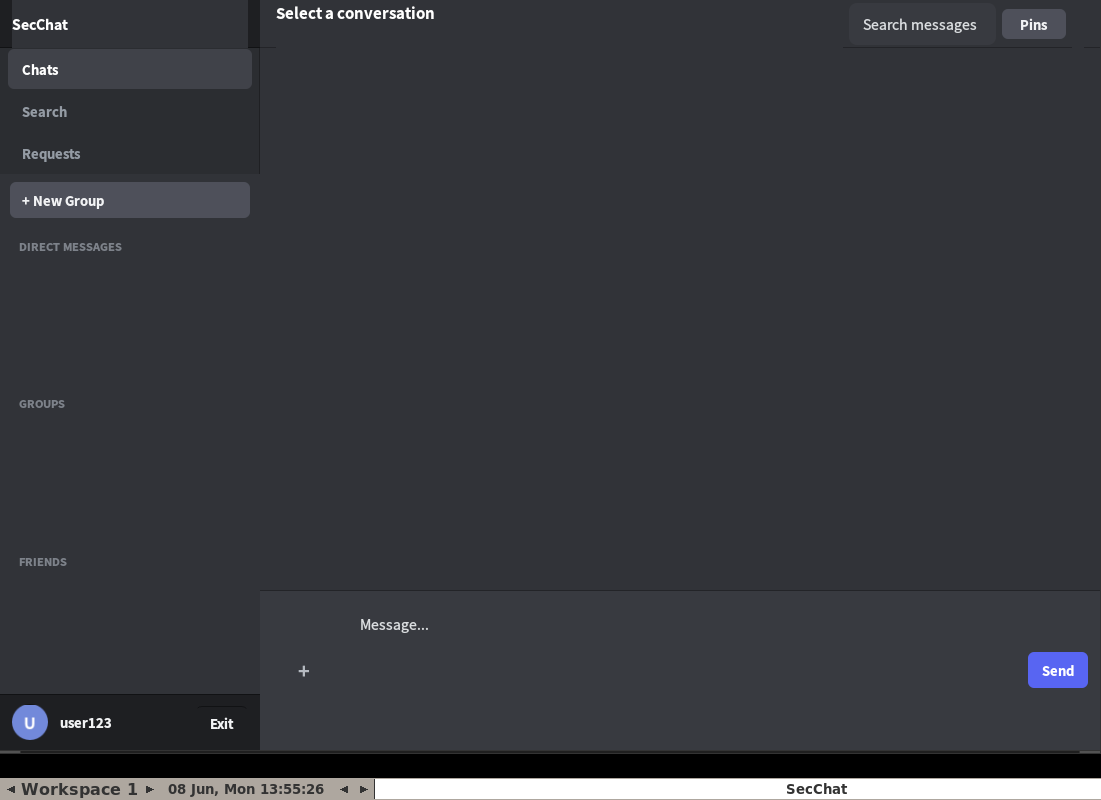
\includegraphics[width=0.95\linewidth]{Figure/ui_login_demo.png}
    \caption{Màn hình đăng nhập trong môi trường VNC}
    \label{fig:ui-login-demo}
\end{figure}

\begin{figure}[H]
    \centering
    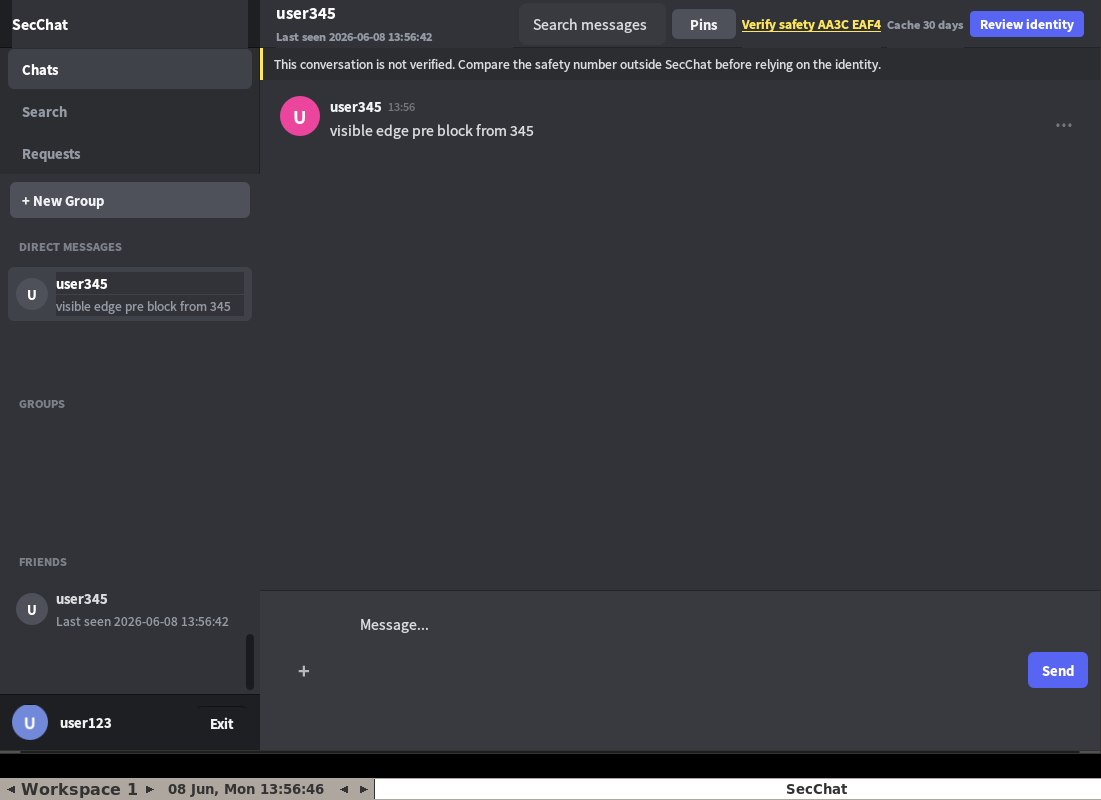
\includegraphics[width=0.95\linewidth]{Figure/ui_friend_list.png}
    \caption{Danh sách bạn bè, DM và group sau khi đăng nhập}
    \label{fig:ui-friend-list}
\end{figure}

\subsection{DM, identity và thao tác tin nhắn}

DM hiển thị header bảo mật, trạng thái review identity, message timeline và vùng nhập tin. Khi hai người dùng chưa review identity, giao diện hiển thị hướng dẫn Review identity.

\begin{figure}[H]
    \centering
    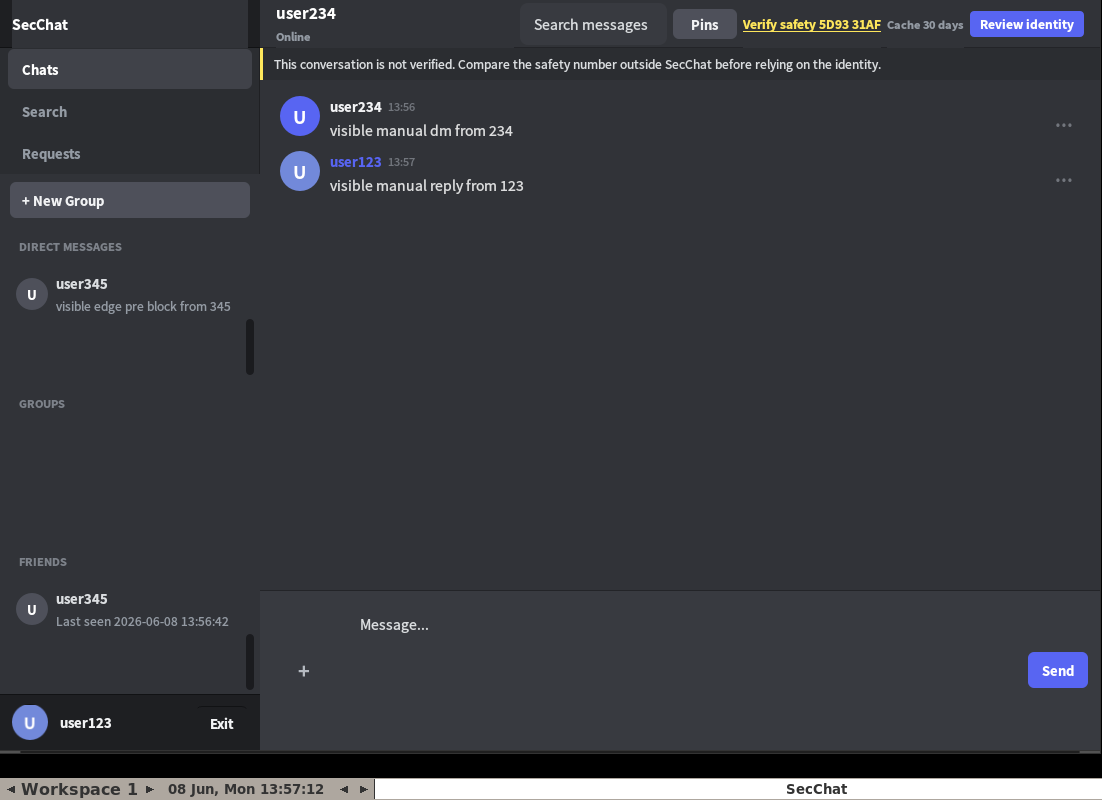
\includegraphics[width=0.95\linewidth]{Figure/ui_dm_current.png}
    \caption{Gửi nhận DM hai chiều với nội dung được giải mã ở client}
    \label{fig:ui-dm-current}
\end{figure}

\begin{figure}[H]
    \centering
    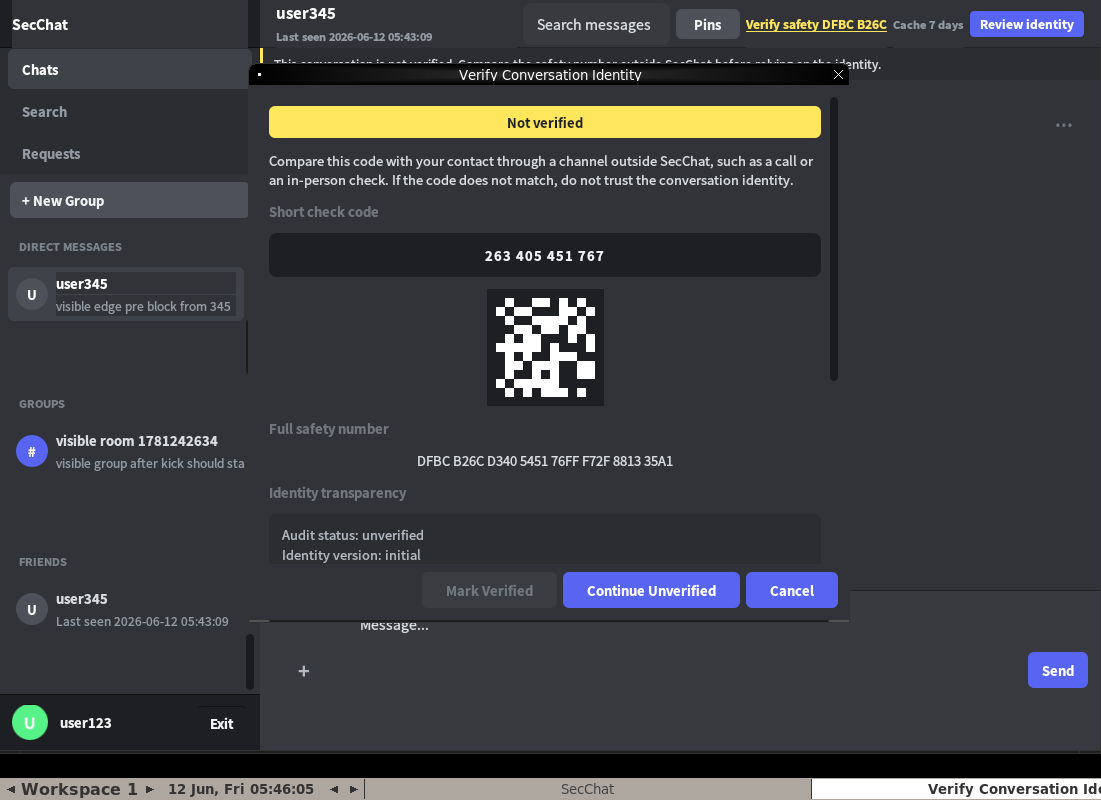
\includegraphics[width=0.95\linewidth]{Figure/ui_identity_review.png}
    \caption{Màn hình kiểm tra safety code trong DM}
    \label{fig:ui-identity-review}
\end{figure}

\begin{figure}[H]
    \centering
    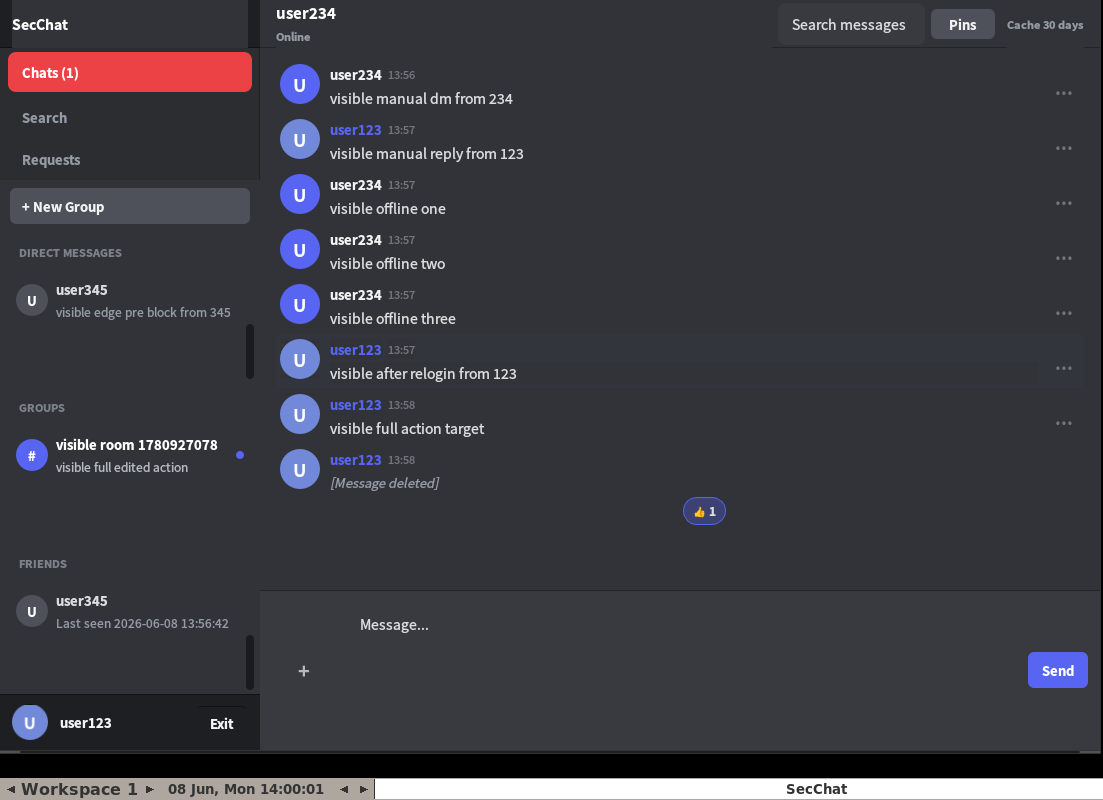
\includegraphics[width=0.95\linewidth]{Figure/ui_message_actions_current.png}
    \caption{Popover thao tác tin nhắn}
    \label{fig:ui-message-actions}
\end{figure}

\begin{figure}[H]
    \centering
    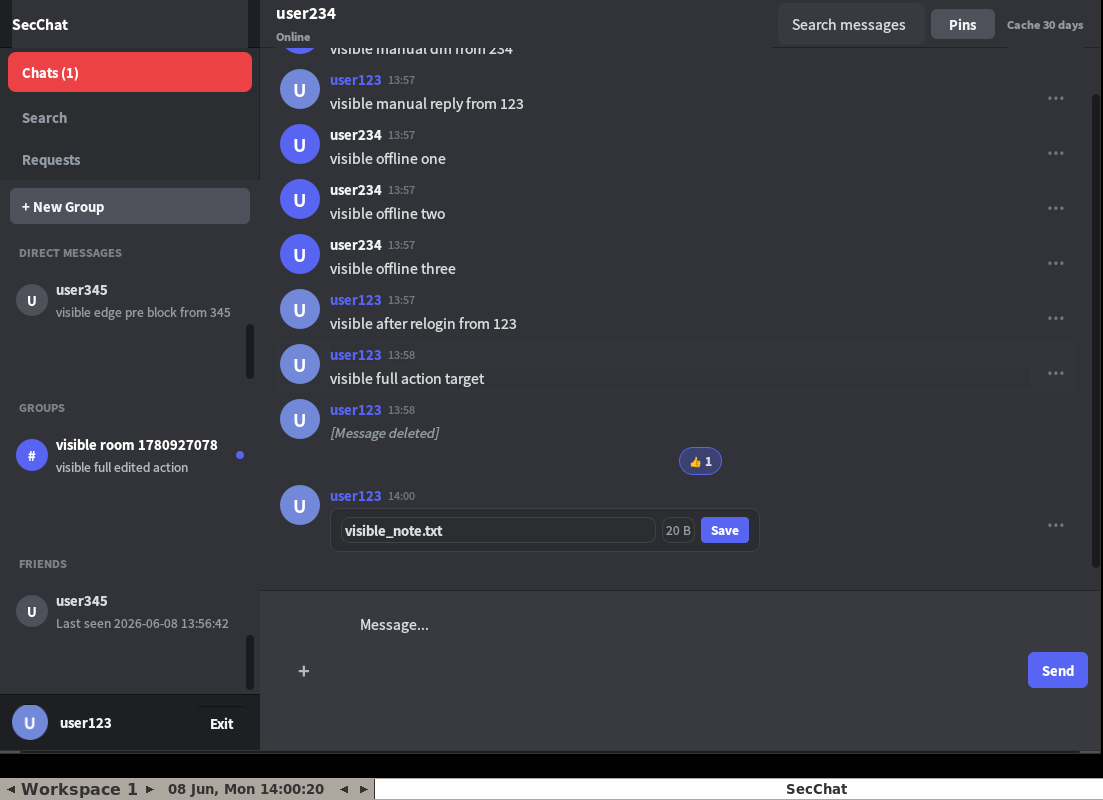
\includegraphics[width=0.95\linewidth]{Figure/ui_file_attachment_current.png}
    \caption{Gửi file trong hội thoại}
    \label{fig:ui-file-attachment}
\end{figure}

\subsection{Group chat và quản lý thành viên}

Group chat hiển thị trạng thái MLS/PQ ở header. Thay đổi member, role và thông tin group xuất hiện trong timeline như system event ổn định.

\begin{figure}[H]
    \centering
    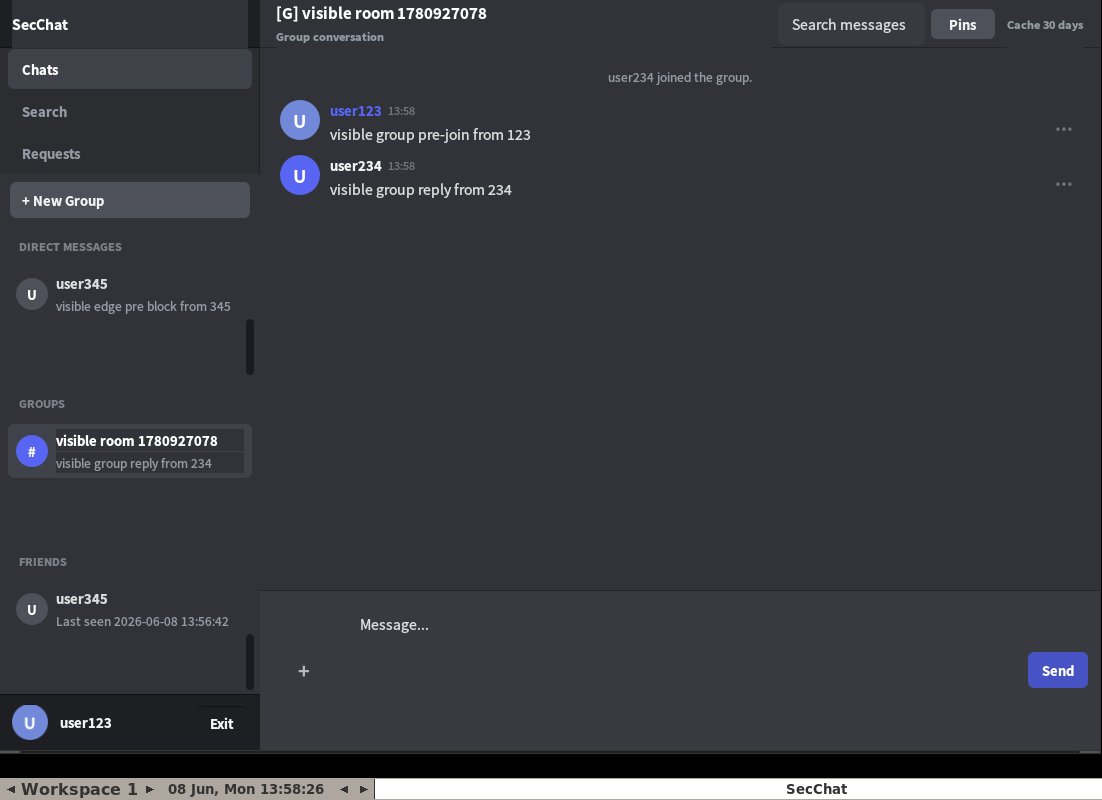
\includegraphics[width=0.95\linewidth]{Figure/ui_group_current.png}
    \caption{Màn hình group chat với trạng thái MLS/PQ}
    \label{fig:ui-group-current}
\end{figure}

\begin{figure}[H]
    \centering
    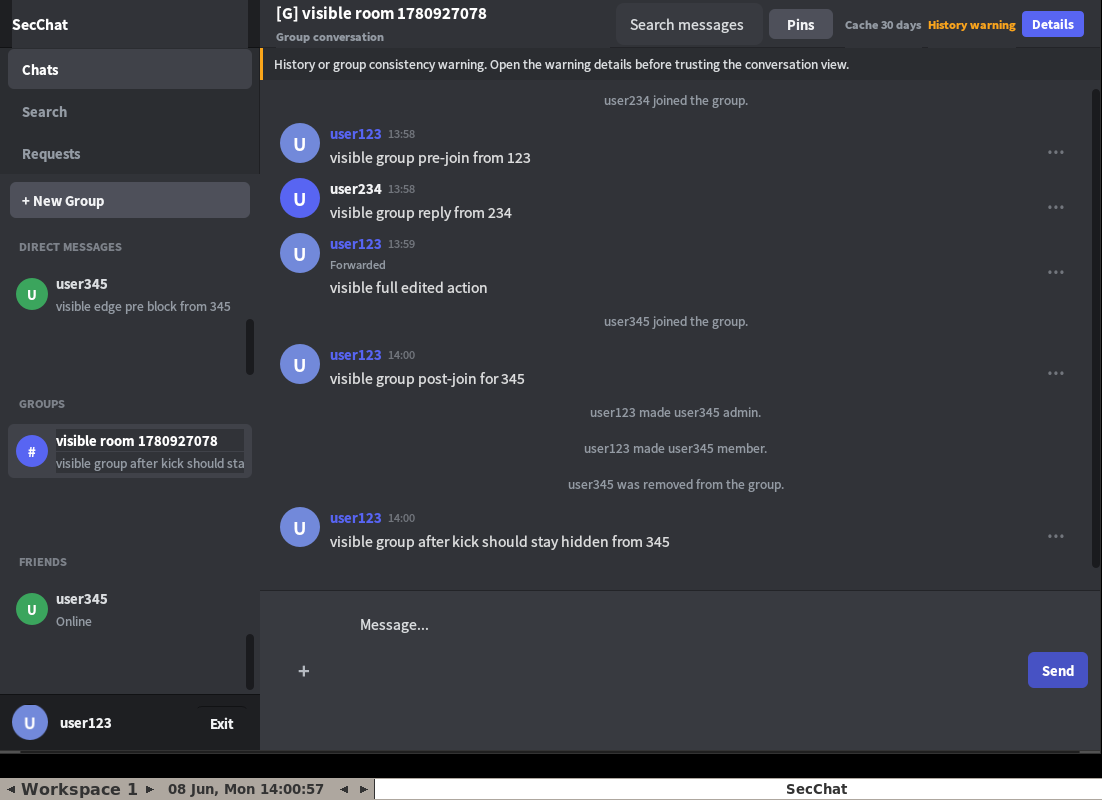
\includegraphics[width=0.95\linewidth]{Figure/ui_group_membership_current.png}
    \caption{Quản lý thành viên, role và system event trong group}
    \label{fig:ui-group-membership}
\end{figure}

\subsection{Backup, profile và trạng thái cuối}

Client cung cấp chức năng quản lý avatar, privacy, cache và backup E2EE trong profile. Backup là file do người dùng giữ, được mã hóa bằng passphrase riêng. Khi restore trên thiết bị khác, client re-wrap local state và publish public material mới mà không đưa plaintext message lên server.

\begin{figure}[H]
    \centering
    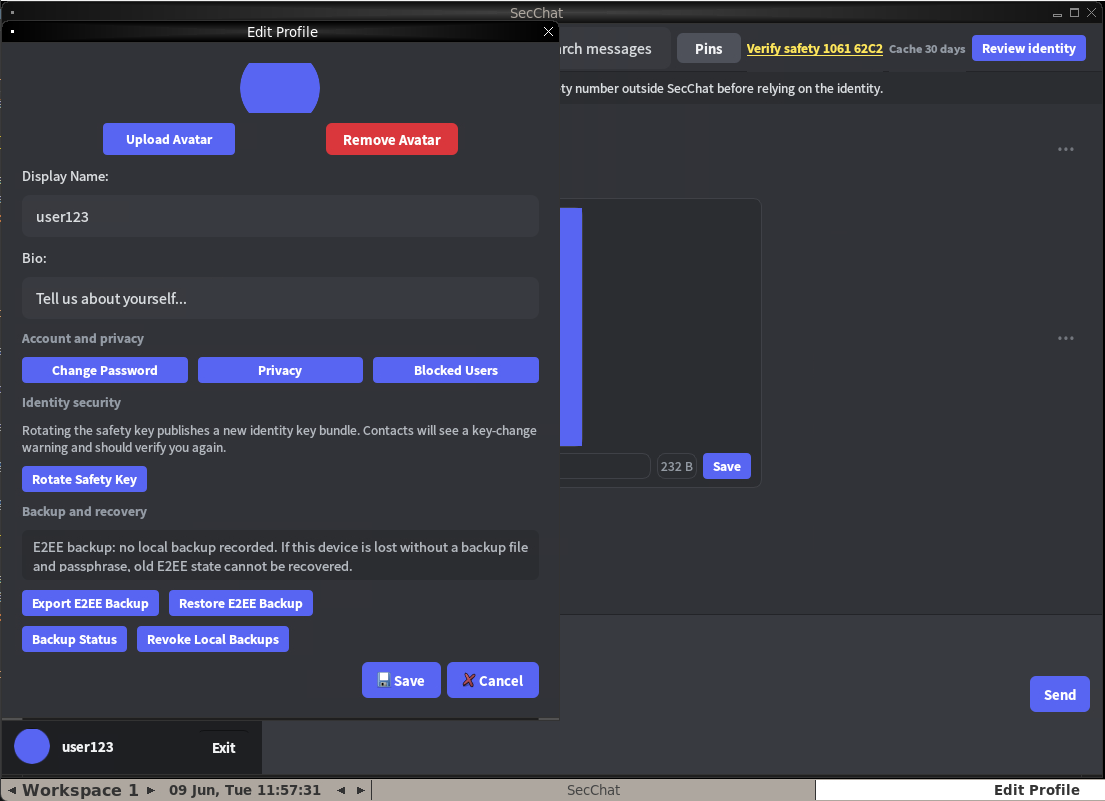
\includegraphics[width=0.95\linewidth]{Figure/3.11.png}
    \caption{Profile, privacy, avatar và backup E2EE}
    \label{fig:ui-profile-backup}
\end{figure}

\begin{figure}[H]
    \centering
    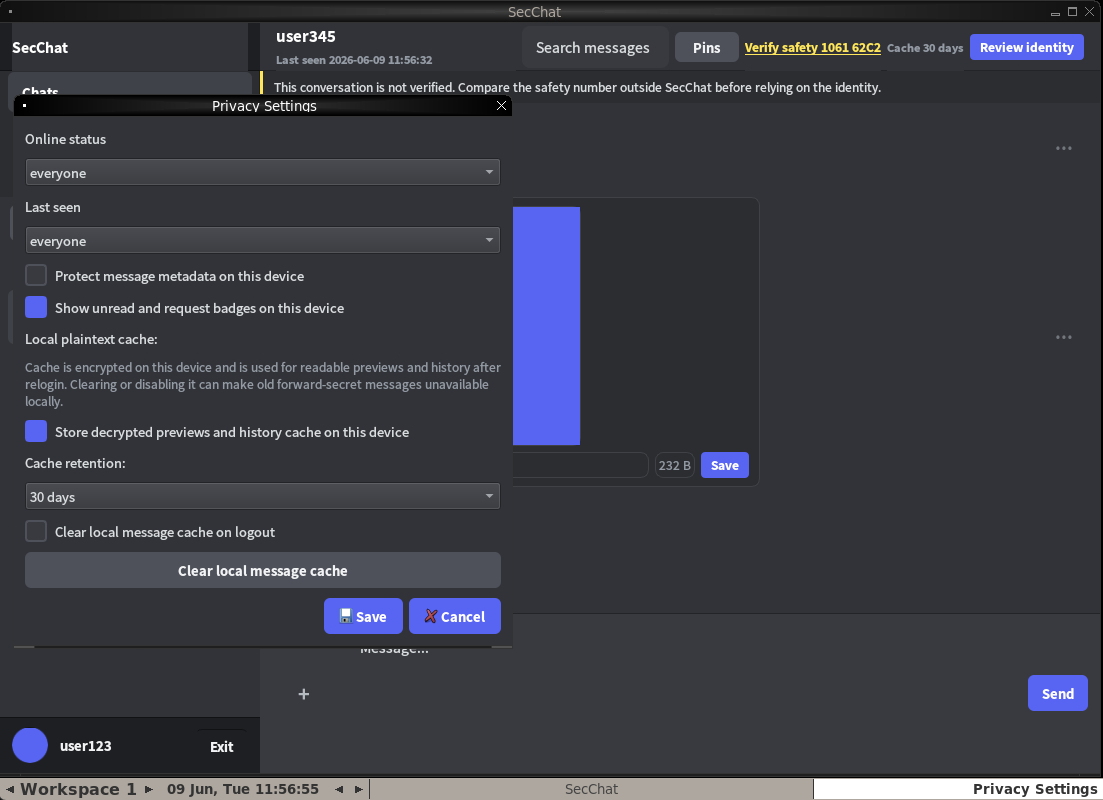
\includegraphics[width=0.95\linewidth]{Figure/3.12.png}
    \caption{Các tùy chọn privacy và cache}
    \label{fig:ui-final-core}
\end{figure}

\section{Kiểm thử chức năng}

Bộ kiểm thử tự động chạy trực tiếp trên stack Docker thật (server C, MySQL, auditor, hai client) và đối chiếu giao thức với server đang chạy. Mỗi file test chạy trong một tiến trình con riêng để một socket treo ở file này không làm hỏng file kế tiếp. Trình điều phối \texttt{tests/run\_all\_tests.py} gom 19 file thành ba nhóm và in bảng tổng kết. Kết quả: toàn bộ 19/19 file đều PASS, 0 fail (Bảng~\ref{tab:functional-test-summary}).

\begin{table}[H]
    \centering
    \small
    \begin{tabularx}{\linewidth}{|p{0.22\linewidth}|c|X|c|}
        \hline
        \textbf{Nhóm} & \textbf{Số file} & \textbf{Nội dung kiểm tra} & \textbf{KQ} \\
        \hline
        Tích hợp & 4 & Domain layer, auth/kết bạn, presence/metrics/search, chặn \& disappearing. & 4/4 \\
        \hline
        Server contract & 13 & HTTP control plane, conv prefs, privacy, multi-session, đếm metrics, giới hạn input, notification, avatar, saved messages, rate limit, identity audit, secure protocol (server), fault injection. & 13/13 \\
        \hline
        Crypto contract & 2 & Bắt tay PQXDH \& Double Ratchet, crypto session. & 2/2 \\
        \hline
        \textbf{Tổng} & \textbf{19} & & \textbf{100\%} \\
        \hline
    \end{tabularx}
    \caption{Tổng hợp kết quả kiểm thử tự động}
    \label{tab:functional-test-summary}
\end{table}

Ảnh chụp màn hình terminal của một phiên chạy trình điều phối \texttt{tests/run\_all\_tests.py} được trình bày ở Hình~\ref{fig:test-run-terminal}.

\begin{figure}[H]
    \centering
    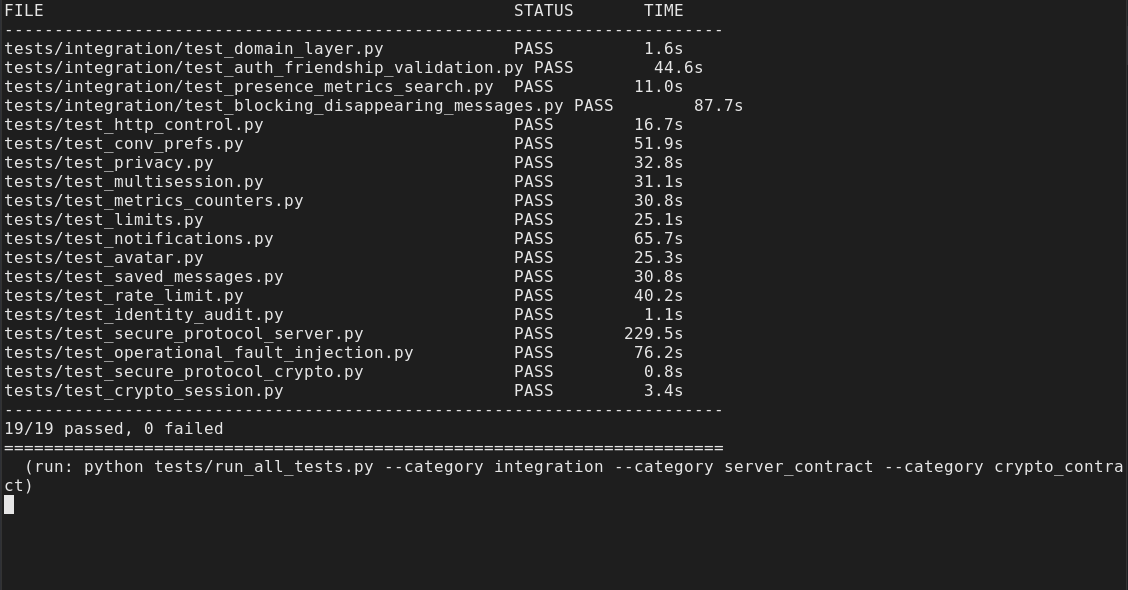
\includegraphics[width=0.95\linewidth]{Figure/ui_test_results.png}
    \caption{Kết quả chạy bộ kiểm thử tự động: 19/19 file PASS, 0 fail}
    \label{fig:test-run-terminal}
\end{figure}

Mỗi file lại gồm nhiều test-case con. Ví dụ nhóm kiểm tra tầng dữ liệu (domain) in chi tiết từng khẳng định:

\begin{figure}[H]
    \centering
    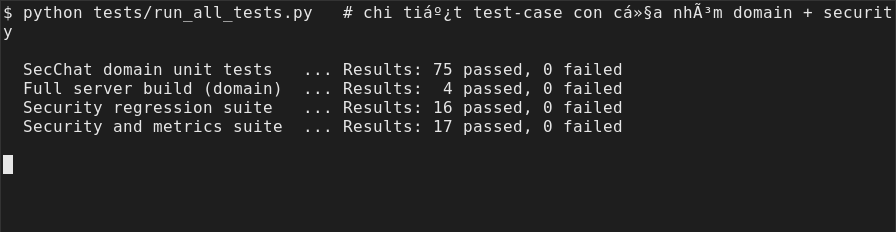
\includegraphics[width=0.78\linewidth]{Figure/ui_test_subsuites.png}
    \caption{Chi tiết test-case con: domain (75), build server (4), an toàn (16), metrics (17) đều PASS.}
    \label{fig:test-subsuites}
\end{figure}

\subsection{Kiểm thử thuộc tính an toàn}

Vì đây là hệ thống bảo mật, ngoài kiểm thử chức năng còn có các kiểm thử đối kháng: cố tình thực hiện thao tác không hợp lệ để xác nhận hệ thống từ chối đúng. Bảng~\ref{tab:security-properties} liệt kê các thuộc tính an toàn cốt lõi cùng test xác minh và kết quả.

\begin{longtable}{|p{0.30\linewidth}|p{0.34\linewidth}|p{0.12\linewidth}|c|}
\caption{Kiểm thử các thuộc tính an toàn (đối kháng)}\label{tab:security-properties}\\
\hline
\textbf{Thuộc tính} & \textbf{Cách kiểm} & \textbf{Kỳ vọng} & \textbf{KQ} \\ \hline
\endfirsthead
\hline
\textbf{Thuộc tính} & \textbf{Cách kiểm} & \textbf{Kỳ vọng} & \textbf{KQ} \\ \hline
\endhead
Server không lưu plaintext & truy vấn bảng \texttt{messages} sau hội thoại & mọi body có prefix \texttt{S3*} & Đạt \\ \hline
Body sai prefix / plaintext bị từ chối & gửi body không hợp lệ (domain validation) & server trả lỗi, không lưu & Đạt \\ \hline
Người ngoài hội thoại không thao tác được & non-member gọi \texttt{pin\_message}/history & bị từ chối & Đạt \\ \hline
Người bị chặn không gửi/không mở DM & user bị block gửi DM, mở DM mới & bị từ chối & Đạt \\ \hline
Chống brute-force đăng nhập & gửi auth sai liên tục & bị rate limit & Đạt \\ \hline
Edit không ghi đè bản gốc & chỉnh sửa tin & thêm row event trỏ về gốc & Đạt \\ \hline
Replay ciphertext cũ bị chặn & gửi lại tin có counter cũ & bị từ chối & Đạt \\ \hline
Rotate identity bị phát hiện & đổi identity rồi nhận bundle & audit báo key changed & Đạt \\ \hline
MLS validator từ chối commit sai & nạp commit/group state không hợp lệ & bị từ chối & Đạt \\ \hline
Phục hồi khi DB/server gián đoạn & tạm dừng DB/server giữa phiên & client báo lỗi rõ, không hỏng state & Đạt \\ \hline
\end{longtable}

Bằng chứng trực tiếp cho thuộc tính ``server không lưu plaintext'': sau một đợt chạy có cả nhắn tin riêng (DM) và nhắn nhóm, truy vấn thẳng bảng \texttt{messages} trong MySQL cho thấy mọi trường \texttt{body} còn lưu đều là ciphertext có prefix giao thức, không có bản rõ. Tin mở đầu mỗi cuộc DM mang prefix \texttt{S3PQI} (gói kèm transcript bắt tay PQXDH); các tin DM tiếp theo mang \texttt{S3DR} (sau khi đã vào Double Ratchet); tin nhóm mang \texttt{S3MLS} (MLS) - tất cả đều ở dạng base64:

\begin{figure}[H]
    \centering
    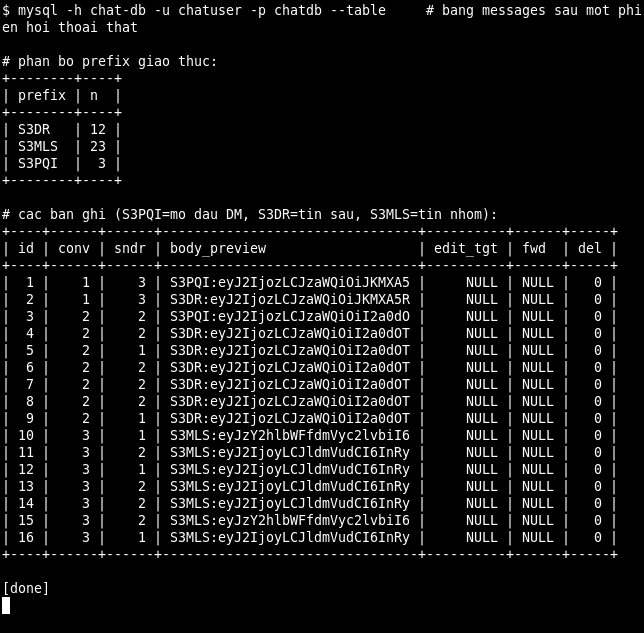
\includegraphics[width=0.82\linewidth]{Figure/ui_db_ciphertext.png}
    \caption{Bằng chứng server không lưu plaintext: truy vấn bảng \texttt{messages}; mọi \texttt{body} là ciphertext có prefix giao thức (\texttt{S3PQI} mở đầu DM, \texttt{S3DR} các tin sau, \texttt{S3MLS} tin nhóm).}
    \label{fig:db-ciphertext}
\end{figure}

\section{Kiểm toán mã nguồn server}

Server viết bằng C nên ngoài kiểm thử chức năng cần kiểm toán an toàn bộ nhớ ở tầng mã nguồn. Các lớp rủi ro cao được tập trung kiểm tra: WebSocket frame parser, JSON command parser, đường lỗi database và MLS validator. Bảng~\ref{tab:source-audit} tổng hợp phương pháp và kết quả định lượng (chạy trong container server).

Các công cụ dùng đều là công cụ kiểm thử mã C tiêu chuẩn, được giới bảo mật tin dùng: cppcheck (phân tích tĩnh), AddressSanitizer/UndefinedBehaviorSanitizer của Clang (phát hiện lỗi bộ nhớ và hành vi không xác định lúc chạy), và libFuzzer (fuzzing dẫn hướng theo độ phủ). Bảng~\ref{tab:source-audit} tổng hợp phương pháp và số liệu định lượng thu được khi chạy trong container server.

\begin{table}[H]
    \centering
    \small
    \begin{tabularx}{\linewidth}{|p{0.24\linewidth}|p{0.30\linewidth}|X|c|}
        \hline
        \textbf{Hạng mục} & \textbf{Công cụ / phương pháp} & \textbf{Số liệu thực đo} & \textbf{KQ} \\
        \hline
        Lỗi bộ nhớ / hành vi không xác định & Clang AddressSanitizer + UBSan, chạy \texttt{make asan\_test\_domain} & biên dịch sạch, chạy hết & 75/75, 0 lỗi \\
        \hline
        Phân tích tĩnh & cppcheck (error/warning/performance/ portability/style) & 36/36 file \texttt{.c} & 0 cảnh báo \\
        \hline
        WebSocket frame parser & libFuzzer \texttt{fuzz\_ws\_frame} (+ASan+UBSan) & 30.000 iter, cov 64, RSS $\approx$40\,MB & 0 crash \\
        \hline
        JSON command parser & libFuzzer \texttt{fuzz\_json\_validation} (+ASan+UBSan) & 30.000 iter, cov 700, RSS $\approx$132\,MB & 0 crash \\
        \hline
    \end{tabularx}
    \caption{Kết quả kiểm toán mã nguồn server}
    \label{tab:source-audit}
\end{table}

Output thực tế của bốn bước định lượng:

\begin{figure}[H]
    \centering
    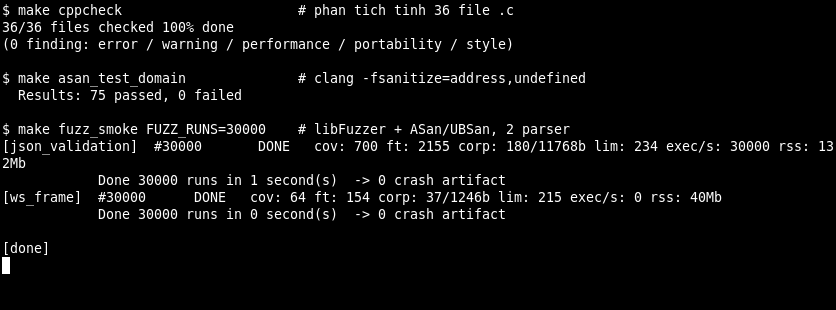
\includegraphics[width=0.86\linewidth]{Figure/ui_c_audit.png}
    \caption{Kiểm toán mã C trong container: cppcheck 36/36, ASan/UBSan 75/75, libFuzzer 30k$\times$2 0 lỗi, 0 crash.}
    \label{fig:c-audit}
\end{figure}

\subsection{Kiểm thử group MLS}

Phần MLS được hiện thực bằng OpenMLS - thư viện tham chiếu cho RFC 9420. Lệnh \texttt{secchat\_mls\_bridge selftest} chạy một vòng đầy đủ: tạo group, thêm member, phát hành Welcome, gửi application message và remove member; đồng thời kiểm tra validator chấp nhận trạng thái hợp lệ và từ chối commit giả mạo. Output JSON thực tế xác nhận ciphersuite hybrid X-Wing và các tính chất đã nêu:

\begin{figure}[H]
    \centering
    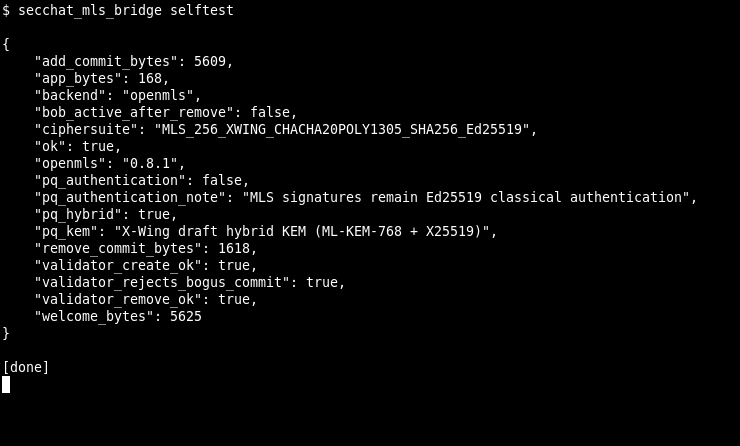
\includegraphics[width=0.74\linewidth]{Figure/ui_mls_selftest.png}
    \caption{Selftest MLS bridge (OpenMLS): ciphersuite X-Wing hybrid; validator chấp nhận state hợp lệ, từ chối commit giả mạo.}
    \label{fig:mls-selftest}
\end{figure}

\section{Đánh giá hiệu năng mật mã}\label{sec:crypto-benchmark}

Phép đo về thời gian và kích thước của các thuật toán mà SecChat sử dụng được thực hiện trong container triển khai (Linux trên Docker/WSL2, máy AMD Ryzen 5 5500U) bằng \texttt{liboqs} 0.15.0 thông qua \texttt{oqs-python} cho ML-KEM và thư viện \texttt{cryptography} cho X25519/Ed25519; mỗi giá trị là trung bình của nhiều lần lặp sau bước khởi động. Output được chụp ở Hình~\ref{fig:crypto-bench}.

\begin{table}[H]
\centering
\renewcommand{\arraystretch}{1.25}
\begin{tabularx}{\linewidth}{|X|r|r|r|r|r|r|}
\hline
\textbf{Nguyên thủy} & \textbf{\makecell{Sinh\\khóa\\(ms)}} & \textbf{\makecell{Mã hóa/\\Ký\\(ms)}} & \textbf{\makecell{Giải mã/\\Xác minh\\(ms)}} & \textbf{\makecell{Khóa\\công khai\\(B)}} & \textbf{\makecell{Khóa\\bí mật\\(B)}} & \textbf{\makecell{Bản mã/\\Chữ ký\\(B)}} \\
\hline
ML-KEM-512  & 0.020 & 0.016 & 0.016 & 800  & 1632 & 768  \\ \hline
ML-KEM-768  & 0.028 & 0.027 & 0.026 & 1184 & 2400 & 1088 \\ \hline
ML-KEM-1024 & 0.038 & 0.033 & 0.036 & 1568 & 3168 & 1568 \\ \hline
X25519 (ECDH)   & 0.041 & 0.031 & --   & 32 & 32 & 32 \\ \hline
Ed25519 (chữ ký) & 0.034 & 0.035 & 0.106 & 32 & 32 & 64 \\ \hline
\end{tabularx}
\caption{Hiệu năng các nguyên thủy mật mã của SecChat (đo trong container Linux). Với KEM, cột ``Mã hóa/Ký'' là Encaps và ``Giải mã/Xác minh'' là Decaps; với X25519 là phép trao đổi khóa.}
\label{tab:crypto-benchmark}
\end{table}

\begin{figure}[H]
    \centering
    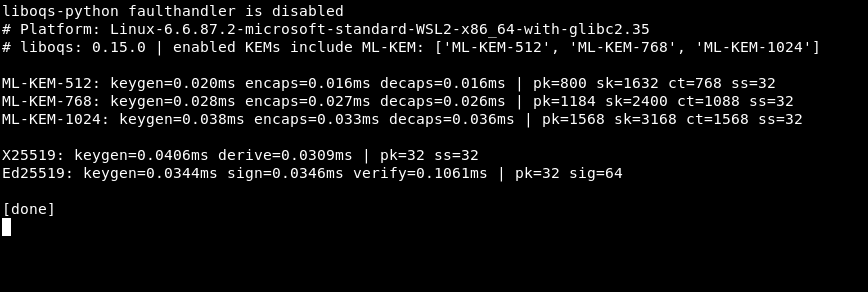
\includegraphics[width=0.92\linewidth]{Figure/ui_crypto_bench.png}
    \caption{Output của phép đo hiệu năng mật mã.}
    \label{fig:crypto-bench}
\end{figure}

Kết quả cho thấy mọi thao tác ML-KEM trong môi trường này đều ở mức vài chục micro giây (dưới một phần nghìn giây), nên việc thêm KEM hậu lượng tử vào bắt tay gần như không gây độ trễ cảm nhận được cho người dùng. Cần lưu ý các số đo X25519/Ed25519 đi qua lớp bao bọc của thư viện \texttt{cryptography} (OpenSSL) nên có thêm chi phí tạo đối tượng, vì vậy thời gian sinh khóa giữa hai họ thuật toán không hoàn toàn so sánh trực tiếp được; điểm quan trọng là tất cả đều ở mức micro giây. Chi phí thực sự nằm ở kích thước: khóa công khai và bản mã ML-KEM vào khoảng 0,8-1,6 KB, lớn hơn nhiều so với 32 byte của X25519, nhưng vẫn nhỏ so với một tin nhắn hay tệp đính kèm thông thường và hoàn toàn chấp nhận được với ứng dụng desktop. Vì SecChat dùng cấu trúc hybrid (X25519 cùng ML-KEM cho DM, và X-Wing = X25519 + ML-KEM-768 cho nhóm), tổng chi phí chỉ là phép cộng của hai cột tương ứng, đổi lại là khả năng kháng lượng tử cho khâu thiết lập khóa.


\section{Quan sát vận hành}

Để minh họa việc quan sát vận hành trực tiếp, sinh một lượng traffic ở mức bình thường rồi giữ các kết nối mở trong lúc chụp màn hình. Kịch bản tải gồm 5 client đăng ký và đăng nhập; mỗi client mở một kết nối khi đăng ký và một kết nối cho phiên làm việc, nên tổng cộng có 10 lượt kết nối được chấp nhận nhưng tối đa chỉ 6 kết nối tồn tại đồng thời. Năm client này tạo 5 quan hệ bạn bè, mở một cuộc DM hai chiều giữa hai người (mỗi bên gửi 5 tin) kèm một lượt sửa, một lượt xóa và một lượt thả cảm xúc, thêm một cuộc DM một chiều 5 tin, lập một nhóm MLS gồm 3 thành viên, rồi đọc inbox và tìm kiếm người dùng (sinh truy vấn cơ sở dữ liệu). Sau khi sinh xong, 5 kết nối được giữ mở để dashboard hiển thị đồng thời cả \emph{active connections} lẫn các bộ đếm tích lũy. Tab \emph{Metrics} của server GUI tự cập nhật mỗi 2 giây bằng cách đọc \texttt{/metrics}; các bộ đếm là tích lũy kể từ khi server khởi động và phiên đo này bắt đầu từ trạng thái đếm bằng 0. Hình~\ref{fig:ui-server-metrics-ch3} là ảnh chụp dashboard, còn Bảng~\ref{tab:ops-metrics} là số liệu \texttt{/metrics} đọc đúng thời điểm chụp.

\begin{table}[H]
    \centering
    \small
    \begin{tabular}{|p{0.50\linewidth}|p{0.38\linewidth}|}
        \hline
        \textbf{Chỉ số (phiên theo dõi)} & \textbf{Giá trị thực đo} \\
        \hline
        Phiên xác thực xử lý & 5 (ok 5 / fail 0 / rate-limited 0) \\
        \hline
        Tài khoản đăng ký & 5 \\
        \hline
        Message gửi / sửa / xóa & 16 / 1 / 1 \\
        \hline
        Tìm kiếm người dùng / bị giới hạn & 3 / 0 \\
        \hline
        Nhóm tạo / reaction & 1 / 1 \\
        \hline
        Kết nối chấp nhận / đỉnh đồng thời / đang mở & 10 / 6 / 5 \\
        \hline
        WebSocket frame nhận / gửi & 58 / 90 \\
        \hline
        Truy vấn cơ sở dữ liệu / lỗi & 41 / \textbf{0} \\
        \hline
        Độ trễ TB auth / gửi tin / DB & 218\,ms / 26\,ms / 11\,ms \\
        \hline
    \end{tabular}
    \caption{Số liệu /metrics màn hình quan sát}
    \label{tab:ops-metrics}
\end{table}

\begin{figure}[H]
    \centering
    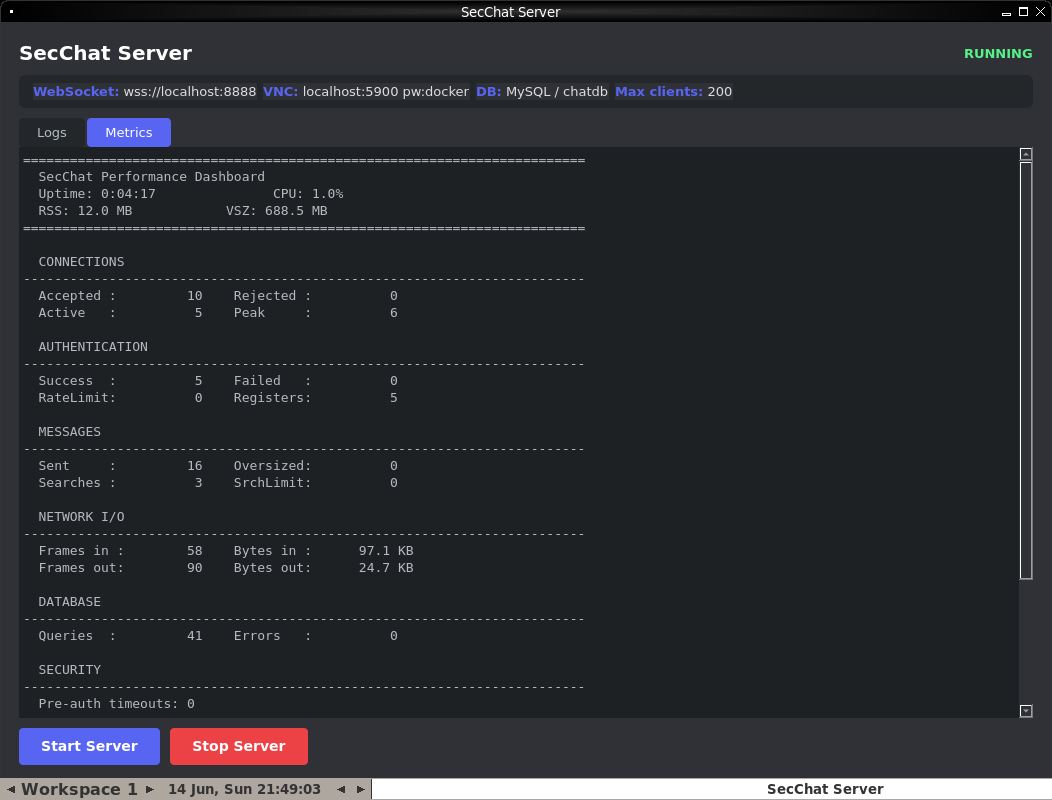
\includegraphics[width=0.95\linewidth]{Figure/ui_server_metrics.png}
    \caption{Ảnh GUI metric của server.}
    \label{fig:ui-server-metrics-ch3}
\end{figure}

Tổng hợp lại, các yêu cầu chính của sản phẩm đã được kiểm chứng: server không lưu plaintext message, DM dùng bắt tay hậu lượng tử và Double Ratchet, group dùng MLS X-Wing hybrid, server validate public MLS state trước khi thay đổi membership, timeline group giữ đúng thứ tự system event, unread state ổn định theo message id và restore E2EE hoạt động trong kịch bản nhiều thiết bị.


\section{Đánh giá bảo mật}

\subsection{Nội dung tin nhắn}

DM dùng bắt tay PQXDH-style để thiết lập secret ban đầu, sau đó dùng Double Ratchet cho từng message. Group dùng MLS theo RFC 9420 qua OpenMLS cho KeyPackage, Welcome, Commit, GroupInfo và application message. Ciphersuite group là X-Wing hybrid:
\begin{center}
    \small\texttt{MLS\_256\_XWING\_CHACHA20POLY1305\_SHA256\_Ed25519}
\end{center}
Server chỉ lưu ciphertext và public MLS artifact đã validate, không giữ secret giải mã nội dung.

Nếu ciphertext bị sửa trực tiếp trong database hoặc trên đường truyền sau khi ra khỏi TLS, client sẽ không giải mã hợp lệ. Thay vì hiển thị dữ liệu sai, UI phải hiển thị trạng thái không thể decrypt.

\subsection{Kháng lượng tử}

SecChat dùng ML-KEM trong bước thỏa thuận khóa DM, và dùng X-Wing trong MLS group. Đây là mật mã hậu lượng tử chạy bằng phần mềm. Nó khác QKD, vì QKD cần thiết bị vật lý và kênh lượng tử. Trong SecChat, dữ liệu vẫn đi qua mạng TCP/TLS bình thường.

Cơ chế hybrid trộn secret từ ML-KEM với X25519 ở DM, và trộn ML-KEM-768 với X25519 trong X-Wing ở group. Ý nghĩa của hybrid là không đặt toàn bộ niềm tin vào một giả định duy nhất. Nếu máy tính lượng tử trong tương lai phá được X25519 nhưng ML-KEM vẫn an toàn, transcript cũ vẫn có lớp bảo vệ hậu lượng tử. Nếu một giả định hậu lượng tử bị yếu trong tương lai nhưng X25519 vẫn an toàn trước attacker hiện tại, phần cổ điển vẫn đóng góp bảo vệ.

Phần hậu lượng tử của SecChat tập trung vào hai khâu: thiết lập khóa và bảo mật nội dung tin nhắn. Ngược lại, việc xác thực định danh vẫn dựa trên chữ ký Ed25519. Như đã nêu ở Chương 1, Ed25519 là một lược đồ chữ ký trên đường cong elliptic, dựa trên cùng bài toán logarit rời rạc mà thuật toán Shor phá được; do đó Ed25519 không kháng lượng tử, và một máy tính lượng tử đủ mạnh trong tương lai có thể giả mạo chữ ký định danh. Đây cũng là giới hạn của chính giao thức PQXDH mà SecChat tham chiếu: PQXDH chỉ bổ sung lớp hậu lượng tử cho bí mật của khóa phiên, còn phần xác thực lẫn nhau vẫn dựa trên độ khó của logarit rời rạc cổ điển. Vì vậy, phạm vi hậu lượng tử của đồ án tập trung vào cơ chế thiết lập khóa và bảo mật nội dung tin nhắn; thành phần xác thực định danh vẫn dùng chữ ký Ed25519 cổ điển, nên xác thực hậu lượng tử đầy đủ - chẳng hạn thay Ed25519 bằng một chữ ký hậu lượng tử như ML-DSA hoặc SLH-DSA - nằm ngoài phạm vi đồ án và là hướng phát triển tiếp theo.

\subsection{Forward secrecy và post-compromise security}

DM có Double Ratchet state, nên tốt hơn thiết kế dùng một khóa hội thoại cố định. Mỗi message dùng message key được dẫn xuất riêng. Khi ratchet state tiến lên, lộ một key ở thời điểm sau không tự động làm lộ toàn bộ quá khứ.

\subsection{Xác thực danh tính}

Identity key Ed25519 ký các prekey, giúp client phát hiện prekey không khớp với identity được công bố. Safety number giúp hai người dùng so sánh identity của nhau qua kênh khác. Khi một người rotate identity, server ghi sự kiện vào \texttt{identity\_key\_log}, auditor dựng Merkle tree và ký checkpoint. Client kiểm tra inclusion proof khi nhận bundle, lưu lịch sử identity cục bộ và hiển thị trạng thái đã xác minh, cần xác minh, key changed, \texttt{audit\_mismatch} hoặc \texttt{audit\_unavailable} trong danh sách hội thoại. Các trạng thái audit có thêm mã lỗi như identity version không có trong log, identity key không khớp, proof root không khớp, checkpoint rollback, checkpoint split-view, chữ ký checkpoint sai hoặc auditor không truy cập được.

Thao tác Mark Verified ghi nhận rằng người dùng đã so sánh safety number hoặc short check code của hội thoại hiện tại qua kênh ngoài SecChat và thấy khớp. Nó không sinh khóa mới và không làm ciphertext mạnh hơn, nhưng là quyết định quan trọng để người dùng xác nhận danh tính của peer sau cảnh báo. Nếu short check code ở hai phía khác nhau, người dùng không nên mark verified vì điều đó cho thấy hai client không đang nhìn cùng một identity state. Khi identity đổi, trạng thái đã xác minh cũ không còn đủ tin cậy và UI chuyển sang cảnh báo key changed hoặc cảnh báo audit có nguyên nhân cụ thể để người dùng review lại. Nếu người dùng restore đúng identity secret trên thiết bị mới, safety identity không đổi; peer không cần thay key, nhưng vẫn có thể cần kiểm tra lại nếu UI hiển thị cảnh báo do lịch sử identity hoặc checkpoint không đủ tin cậy. Nếu người dùng không restore và chọn rotate safety key, đây là thay đổi identity thật sự và các peer phải xem như một safety number mới.

\subsection{Metadata}

E2EE không che được toàn bộ metadata. Server vẫn biết user id, conversation id, thành viên group, thời điểm gửi, kích thước tương đối của message, trạng thái online, pin, reaction, edit target và một số sự kiện privacy-sensitive nếu người dùng bật chúng. 

Client có một số biện pháp giảm metadata như tắt typing indicator, padding plaintext trước khi mã hóa, kiểm tra consistency của history và kiểm tra commit chain của group. 

Server cũng validate public MLS state để tránh membership bị mutate bởi Commit không hợp lệ, nhưng việc này không ẩn membership khỏi server. 

Những biện pháp này giúp giảm hoặc phát hiện một số rủi ro, nhưng không làm server trở thành không cần tin cậy. Khi phát hiện history, group commit hoặc transcript checkpoint không nhất quán, UI hiển thị cảnh báo kèm nút Details để người dùng xem nguyên nhân cụ thể. Ẩn metadata mạnh hơn cần các kỹ thuật khác như sealed sender, private information retrieval, mix network hoặc delay traffic. Các kỹ thuật đó nằm ngoài phạm vi của đồ án.

\subsection{Local plaintext cache}

Local plaintext cache giúp người dùng đọc lại lịch sử sau relogin, nhất là khi ratchet state không thể decrypt lại mọi message cũ từ đầu. Cache này được mã hóa bằng master key, nên không phải plaintext thô trên ổ đĩa. Tuy nhiên nó vẫn là dữ liệu nhạy cảm. Nếu thiết bị bị chiếm và attacker có được mật khẩu hoặc master key, lịch sử cache có thể bị đọc.

Hệ thống có chính sách cache rõ: người dùng có thể tắt cache toàn cục, tắt cache cho từng conversation nhạy cảm, đặt thời gian giữ cache, xóa cache thủ công và chọn xóa cache khi logout. Cache được đặt theo tài khoản trong thư mục dữ liệu của client, nên tài khoản mới trên cùng thiết bị không được thấy cache của tài khoản cũ và cũng không được xóa cache đó. Khi export backup E2EE, người dùng chọn có đưa message cache vào file backup hay không. Đây là đánh đổi hợp lý cho trải nghiệm desktop giữa sự tiện dụng và bảo vệ dữ liệu cục bộ.

\section{Đánh giá kiến trúc phần mềm}

\subsection{Client}

Client có ranh giới rõ giữa UI, network và crypto engine. Controller chính không trực tiếp giữ toàn bộ file key, ratchet state và cache; phần lớn state nhạy cảm và thao tác mã hóa outbound nằm trong crypto engine. Điều này làm kiến trúc dễ giải thích hơn: UI gửi yêu cầu, network truyền gói, crypto engine giữ khóa và mã hóa.

Một phần decrypt message nhận vào và replay history cũng nằm trong crypto session, nhưng controller UI vẫn điều phối khá nhiều nhánh xử lý live event, history, pending key và cập nhật UI. Vì vậy crypto engine là thành phần sở hữu state nhạy cảm, còn controller UI là lớp phối hợp sự kiện.

\subsection{Server}

Repository  chịu trách nhiệm SQL, services chịu trách nhiệm nghiệp vụ, infra xử lý cấu hình và metrics, transport xử lý socket và HTTP. 

Điểm cần chú ý là server viết bằng C. C cho hiệu năng tốt và kiểm soát thấp tầng, nhưng dễ gặp lỗi memory hoặc string nếu không review kỹ. Với hệ thống bảo mật, cần tiếp tục giữ quy tắc dùng prepared statement, kiểm tra độ dài input và tránh build JSON bằng buffer không đủ kích thước.

\subsection{Cơ sở dữ liệu}

Schema bao phủ nhiều nhu cầu của app: user, profile, friendship, block, conversation, member, message, reaction, pin, notification, key bundle, prekey và public MLS state. Điều này đủ cho một ứng dụng chat desktop có nhiều tính năng.

Một điểm cần quản lý là ranh giới giữa dữ liệu phục vụ giao thức chính và dữ liệu phụ trợ cho vận hành. Những bảng lưu identity, bundle, one-time prekey, notification và message metadata phải có vai trò rõ ràng để tránh nhầm lẫn giữa khóa dùng cho E2EE và metadata server cần để điều phối hệ thống.


\section{Các nguy cơ còn lại}

Hệ thống vẫn còn một số giới hạn. Thứ nhất, group protocol dùng OpenMLS theo RFC 9420 cho flow KeyPackage, Welcome, Commit và application message, với X-Wing draft hybrid ML-KEM-768 + X25519. Đây là bảo vệ hậu lượng tử cho confidentiality, không phải authentication hậu lượng tử. Do X-Wing vẫn là draft trong hệ sinh thái MLS, hệ thống cần kế hoạch migration nếu định danh ciphersuite hoặc encoding thay đổi khi chuẩn cuối cùng ổn định.

Thứ hai, metadata chưa được ẩn. Đây là vấn đề khó và cần thiết kế riêng, không thể giải quyết chỉ bằng cách mã hóa body message.

Thứ ba, local cache giúp trải nghiệm tốt hơn nhưng làm tăng lượng dữ liệu nhạy cảm trên thiết bị. Vì vậy bảo vệ thiết bị, mật khẩu mạnh và khóa màn hình vẫn rất quan trọng.

Thứ tư, hệ thống chưa có multi-device đầy đủ. Một tài khoản chủ yếu gắn với một phiên client active tại một thời điểm. Đổi thiết bị được hỗ trợ ở mức khôi phục identity, công bố bundle mới và đọc lại lịch sử từ cache hoặc backup; hệ thống chưa có danh sách thiết bị, chưa đồng bộ ratchet state liên tục và chưa có cơ chế xác minh chéo giữa các thiết bị. Có thể cải thiện bằng cách cho mỗi thiết bị thêm identity phụ, prekey riêng và cơ chế thêm thiết bị an toàn.

\section{Hướng phát triển}

\subsection{Multi-device}

Hỗ trợ multi-device thực sự sẽ nâng cao trải nghiệm người dùng, nhưng cũng làm tăng độ phức tạp của giao thức và triển khai. Một số ý tưởng có thể nghiên cứu là thiết kế flow thêm thiết bị an toàn, đồng bộ ratchet state qua MLS hoặc server relay, và xác minh chéo identity giữa các thiết bị để phát hiện xâm nhập.

\subsection{Nâng cấp bảo vệ metadata}

Bảo vệ metadata là hướng khó nhưng có giá trị. Một số ý tưởng có thể nghiên cứu là sealed sender, giảm thông tin trong inbox, gom thời điểm gửi, hoặc thiết kế relay không biết đầy đủ quan hệ người gửi-người nhận. Đây nên được xem là một đề tài riêng, vì nó phức tạp hơn nhiều so với mã hóa nội dung.

\subsection{Cải thiện UI và nền tảng}

Có thể cải thiện tìm kiếm lịch sử, preview media, kéo thả nhiều file, trạng thái gửi thất bại, retry, notification và hỗ trợ mobile. Với mobile hoặc web, cần đặc biệt cẩn thận để không làm yếu mô hình E2EE khi chuyển key và local state sang nền tảng mới.

\newpage

\chapter*{Kết luận}
\addcontentsline{toc}{chapter}{Kết luận}
Qua quá trình tìm hiểu, nghiên cứu, thiết kế, triển khai và báo cáo, đồ án đã được hoàn thiện. Đề tài “Xây dựng giao thức nhắn tin an toàn tích hợp giải pháp mật mã hậu lượng tử” đã đạt được một số kết quả nhất định, cụ thể như sau:

\begin{itemize}
    \item Tìm hiểu và hệ thống hóa các kiến thức nền tảng liên quan đến ứng dụng nhắn tin, mã hóa đầu cuối và mật mã kháng lượng tử.
    \item Phân tích yêu cầu và thiết kế kiến trúc cho hệ thống ứng dụng nhắn tin đảm bảo tính bảo mật và riêng tư cho người dùng.
    \item Xây dựng và triển khai ứng dụng nhắn tin với các chức năng cơ bản.
    \item Tích hợp cơ chế mã hóa đầu cuối kết hợp với các thuật toán mật mã hậu lượng tử nhằm nâng cao mức độ an toàn trước các mối đe dọa hiện tại và tương lai.
    \item Thực hiện thử nghiệm và đánh giá một số tính năng cơ bản cũng như hiệu quả hoạt động của hệ thống.
\end{itemize}

Trong tương lai, đề tài có thể tiếp tục được phát triển theo các hướng sau:

\begin{itemize}
    \item Mở rộng ứng dụng với nhiều tính năng nâng cao như gọi thoại và gọi video an toàn.
    \item Nghiên cứu và tích hợp thêm các thuật toán mật mã hậu lượng tử tiên tiến nhằm tăng cường khả năng bảo mật.
    \item Tối ưu hiệu năng hệ thống, giảm độ trễ và nâng cao khả năng mở rộng khi số lượng người dùng tăng cao.
    \item Triển khai hệ thống trong môi trường thực tế và đánh giá trên quy mô lớn hơn.
\end{itemize}

Trong quá trình thực hiện đồ án, mặc dù đã rất cố gắng nhưng do hạn chế về thời gian và kiến thức, đồ án không tránh khỏi những thiếu sót. Em rất mong nhận được sự đóng góp ý kiến và chỉ bảo của các thầy cô và các bạn để đồ án được hoàn thiện hơn.

Em xin chân thành cảm ơn!

\nocite{*}

\addcontentsline{toc}{chapter}{Tài liệu tham khảo}
\bibliography{references}
\bibliographystyle{unsrt}


\end{document}
